% El atlas contiene resultados numéricos y pertenece exclusivamente a la
% salida completa. La guarda interna evita que una inclusión futura
% del módulo pueda incorporarlo por accidente al volumen impreso de estudio.
\ifHAFOdigitalcontent
\section{Atlas de resultados numéricos}
\label{part:atlas}
Las figuras muestran trayectorias, espectros, equilibrios y sondeos de
cuenca de los sistemas estudiados. Los espectros de amplitud obtenidos mediante
FFT y las estimaciones de densidad espectral de potencia se identifican por
separado. Las curvas representan observaciones en intervalos finitos.

\clearpage
\subsection{Chua entero y fraccionario: figuras de referencia}
Incluye Nyquist, transferencia, continuación, atractores, series, diagnósticos espectrales, Matignon y sondeos de cuenca para las rutas de Chua.

\begin{center}
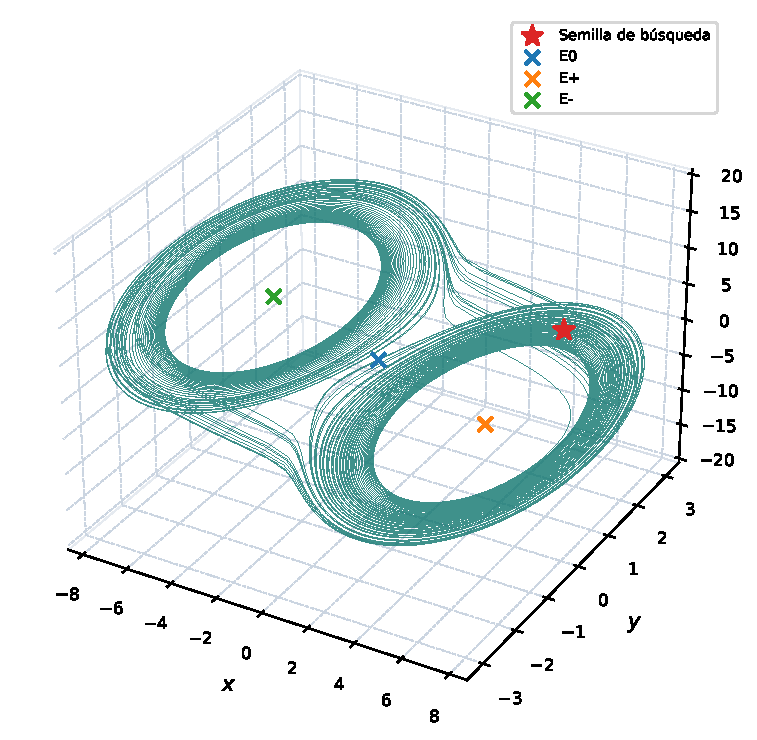
\includegraphics[width=0.94\linewidth,height=0.37\textheight,keepaspectratio]{figures/chua_master/chua_frac_arctan_c590_fig00_initial_seed.pdf}\\[-0.25em]
{\footnotesize Chua arctangente c590: condición inicial y trayectoria de arranque.}
\end{center}
\vfill
\begin{center}
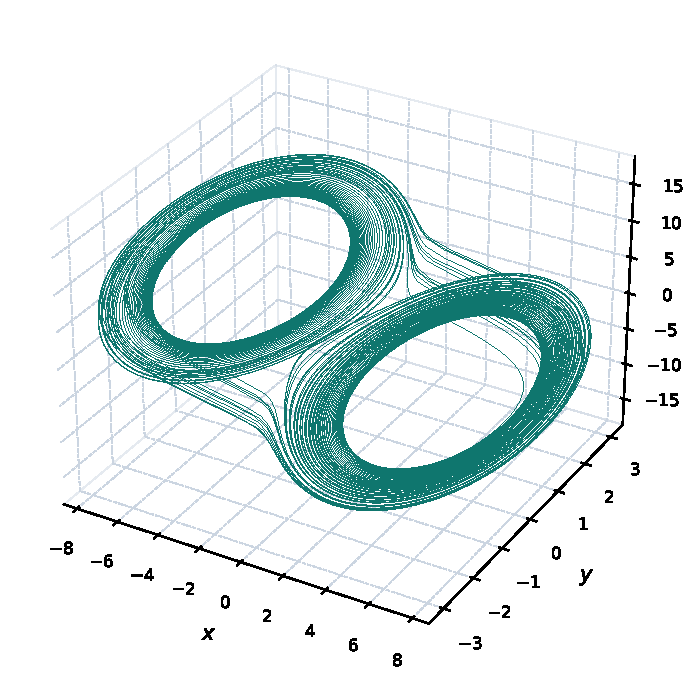
\includegraphics[width=0.94\linewidth,height=0.37\textheight,keepaspectratio]{figures/chua_master/chua_frac_arctan_c590_fig03_attractor.pdf}\\[-0.25em]
{\footnotesize Chua arctangente c590: trayectoria candidata en el espacio de estados.}
\end{center}
\clearpage
\begin{center}
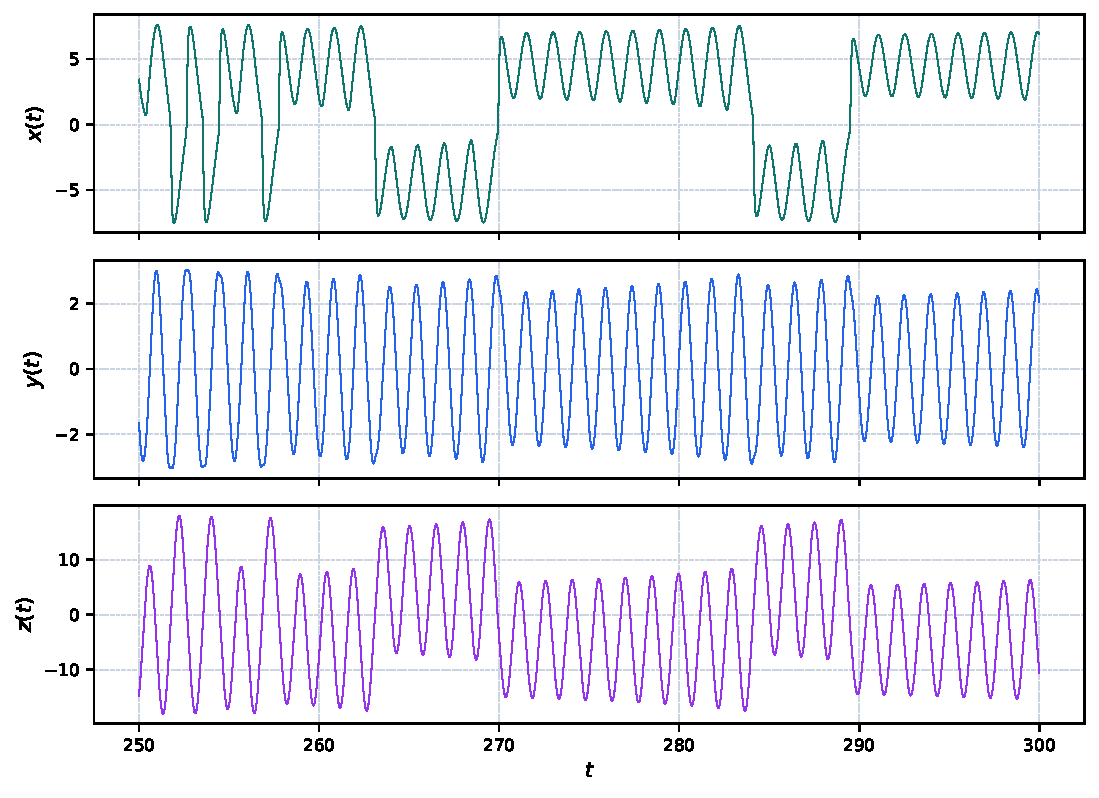
\includegraphics[width=0.94\linewidth,height=0.37\textheight,keepaspectratio]{figures/chua_master/chua_frac_arctan_c590_fig04_timeseries.pdf}\\[-0.25em]
{\footnotesize Chua arctangente c590: series temporales.}
\end{center}
\vfill
\begin{center}
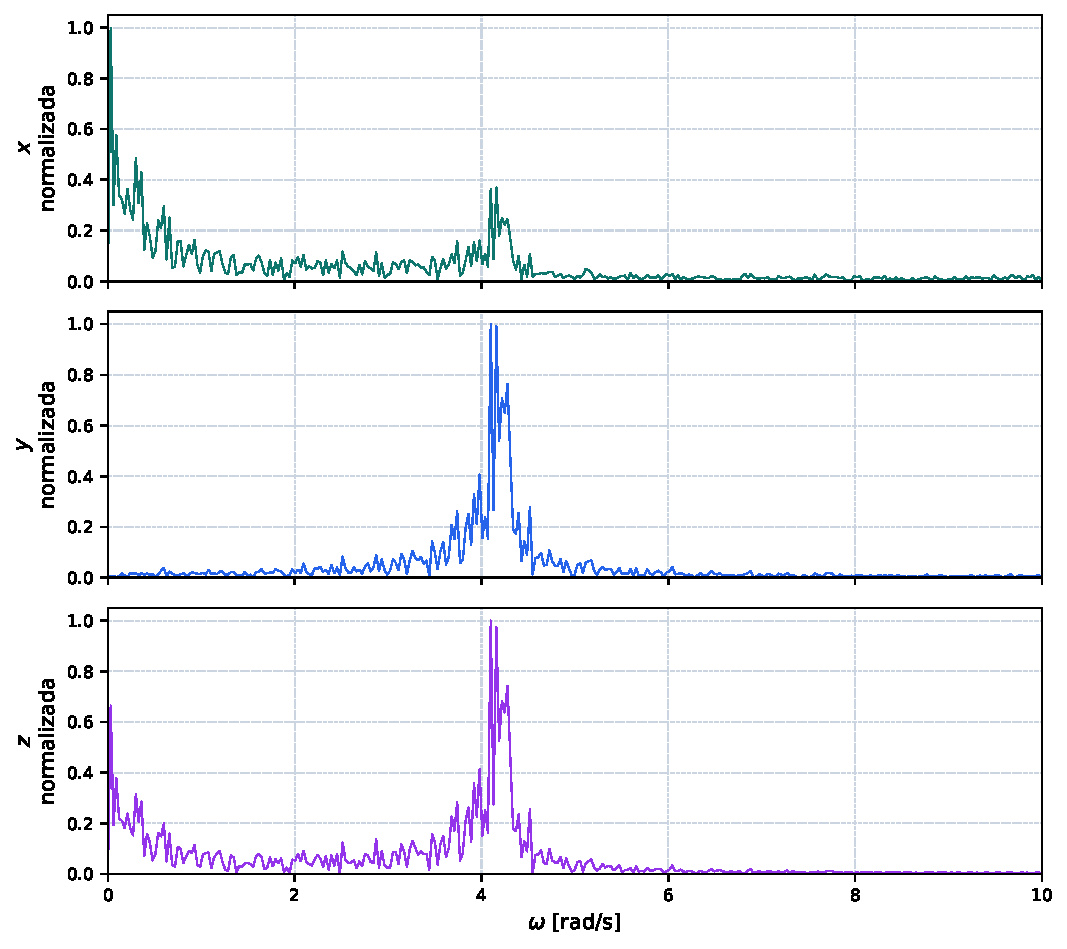
\includegraphics[width=0.94\linewidth,height=0.37\textheight,keepaspectratio]{figures/chua_master/chua_frac_arctan_c590_fig11_fft.pdf}\\[-0.25em]
{\footnotesize Chua arctangente c590: espectro de amplitud.}
\end{center}
\clearpage
\begin{center}
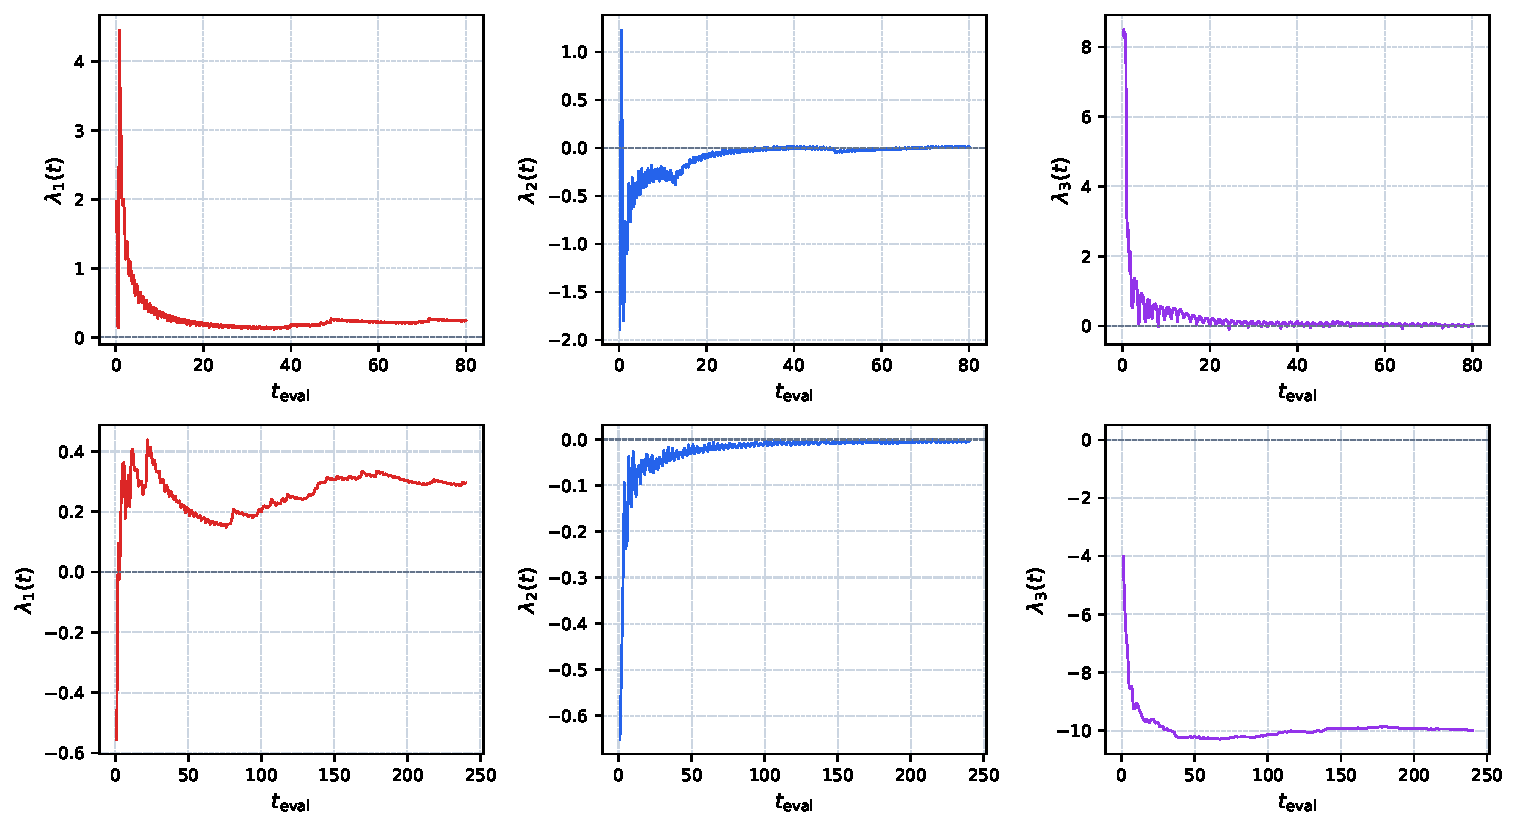
\includegraphics[width=0.94\linewidth,height=0.37\textheight,keepaspectratio]{figures/chua_master/chua_frac_arctan_c590_fig12_lyapunov_two_methods.pdf}\\[-0.25em]
{\footnotesize Chua arctangente c590: comparación de dos estimaciones de Lyapunov.}
\end{center}
\vfill
\begin{center}
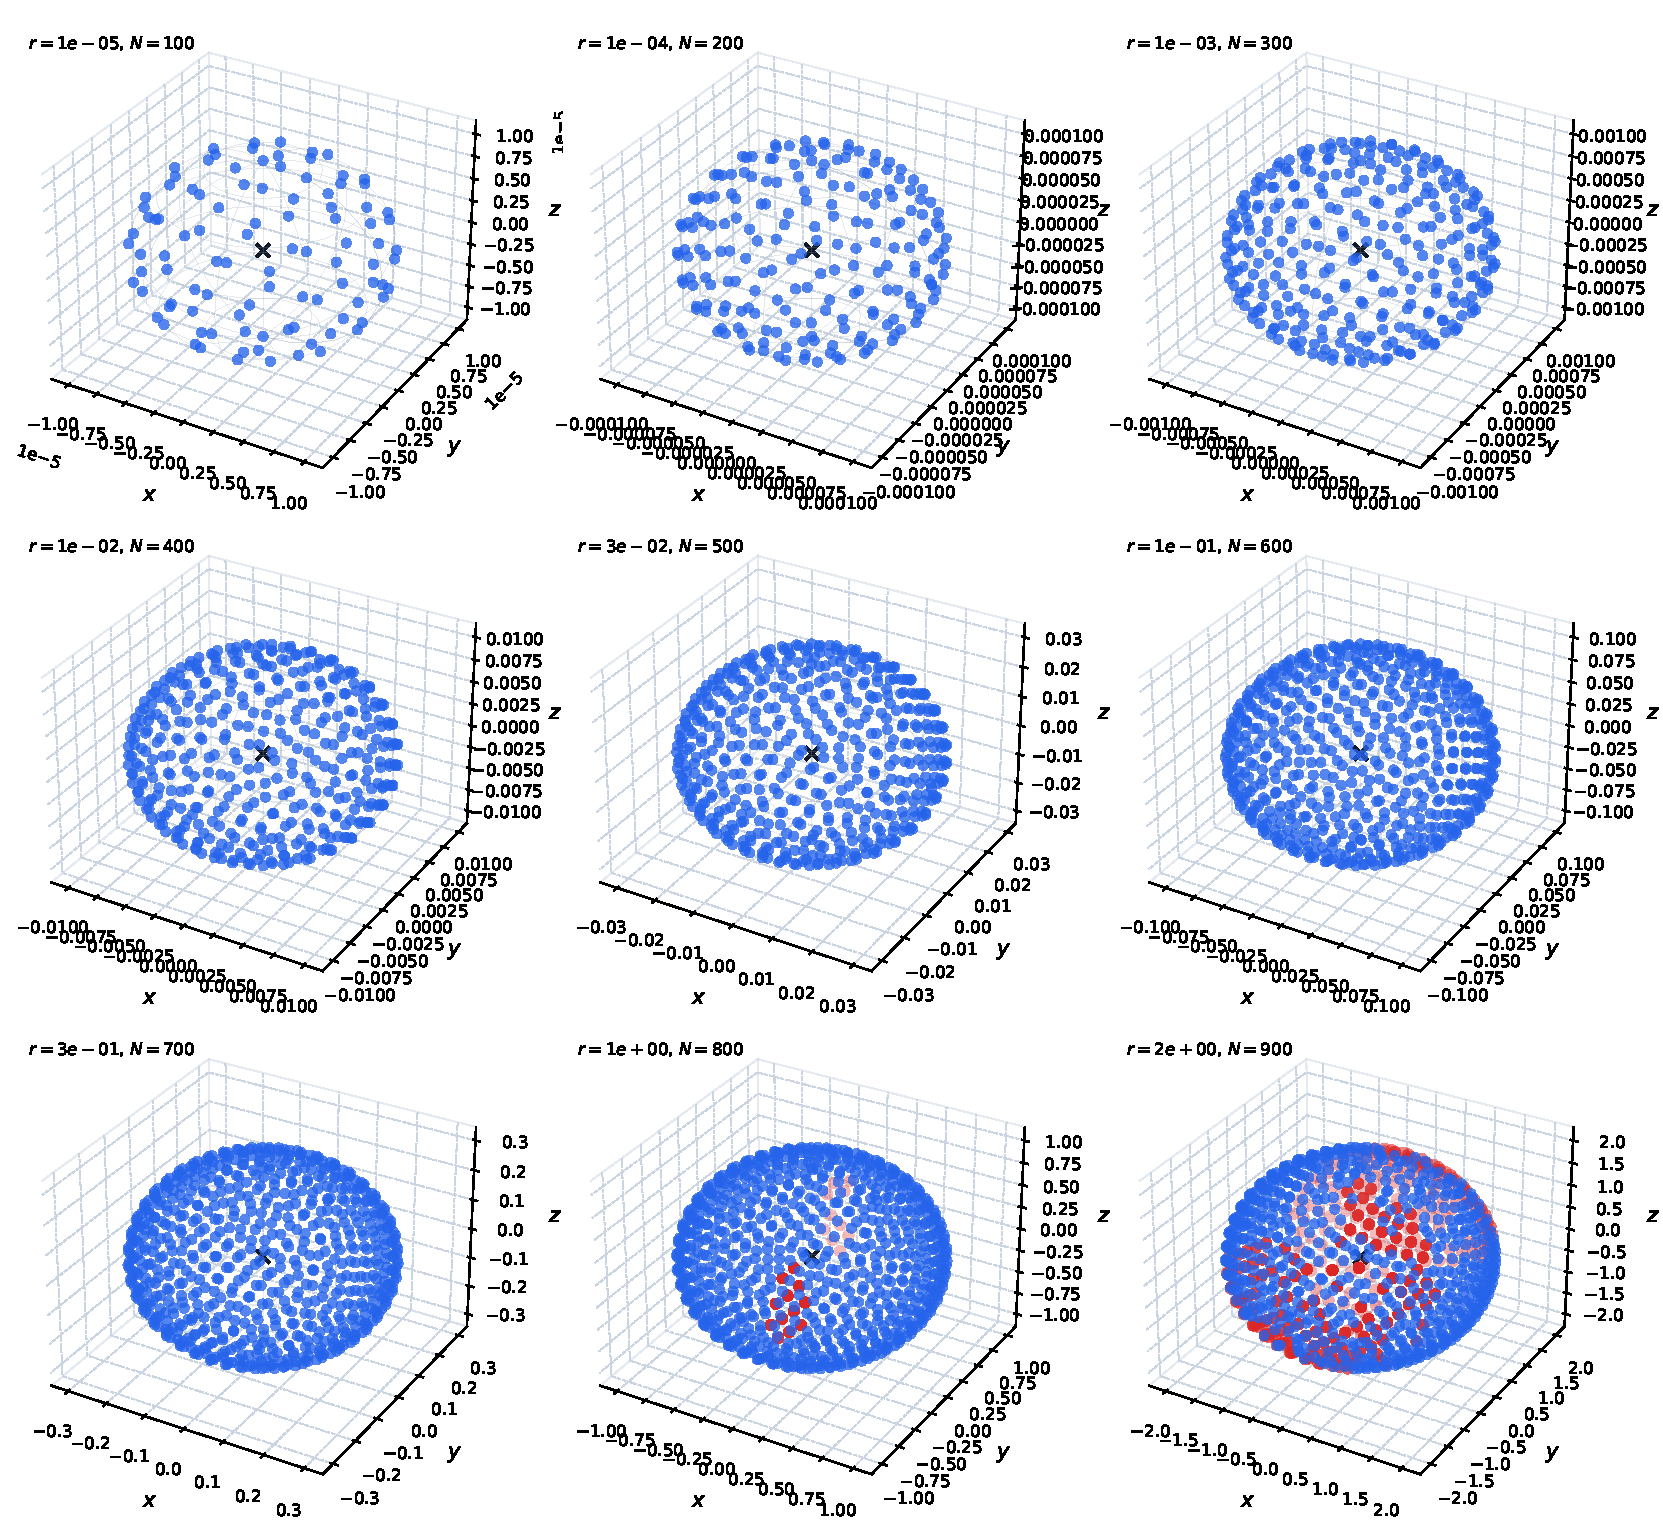
\includegraphics[width=0.94\linewidth,height=0.37\textheight,keepaspectratio]{figures/chua_master/chua_frac_arctan_c590_fig13_E0_hiddenness_spherical_3d.pdf}\\[-0.25em]
{\footnotesize Chua arctangente c590: sondeos esféricos próximos a \(E_0\).}
\end{center}
\clearpage
\begin{center}
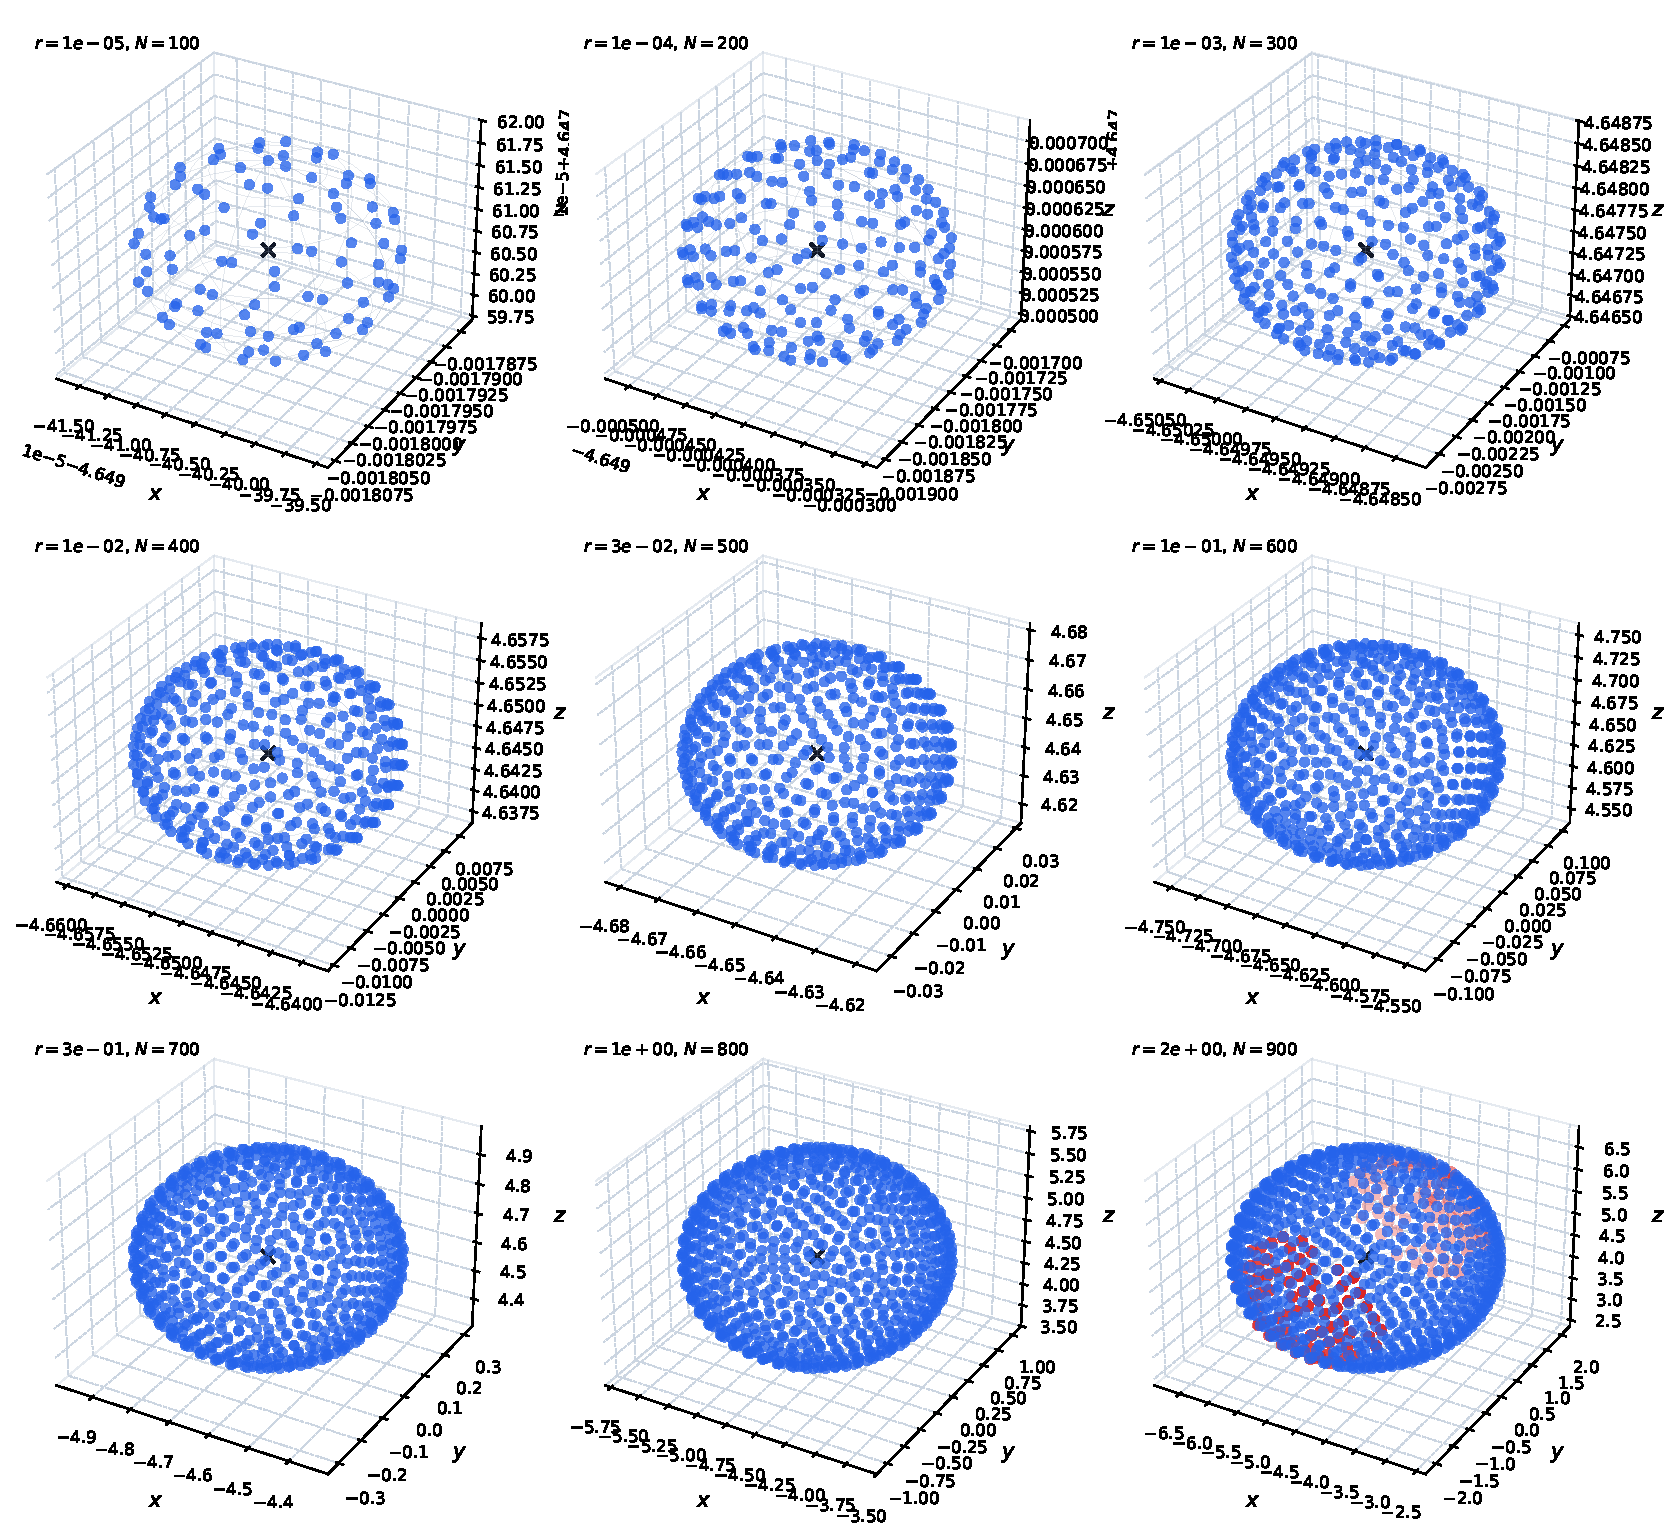
\includegraphics[width=0.94\linewidth,height=0.37\textheight,keepaspectratio]{figures/chua_master/chua_frac_arctan_c590_fig13_Em_hiddenness_spherical_3d.pdf}\\[-0.25em]
{\footnotesize Chua arctangente c590: sondeos esféricos próximos a \(E_-\).}
\end{center}
\vfill
\begin{center}
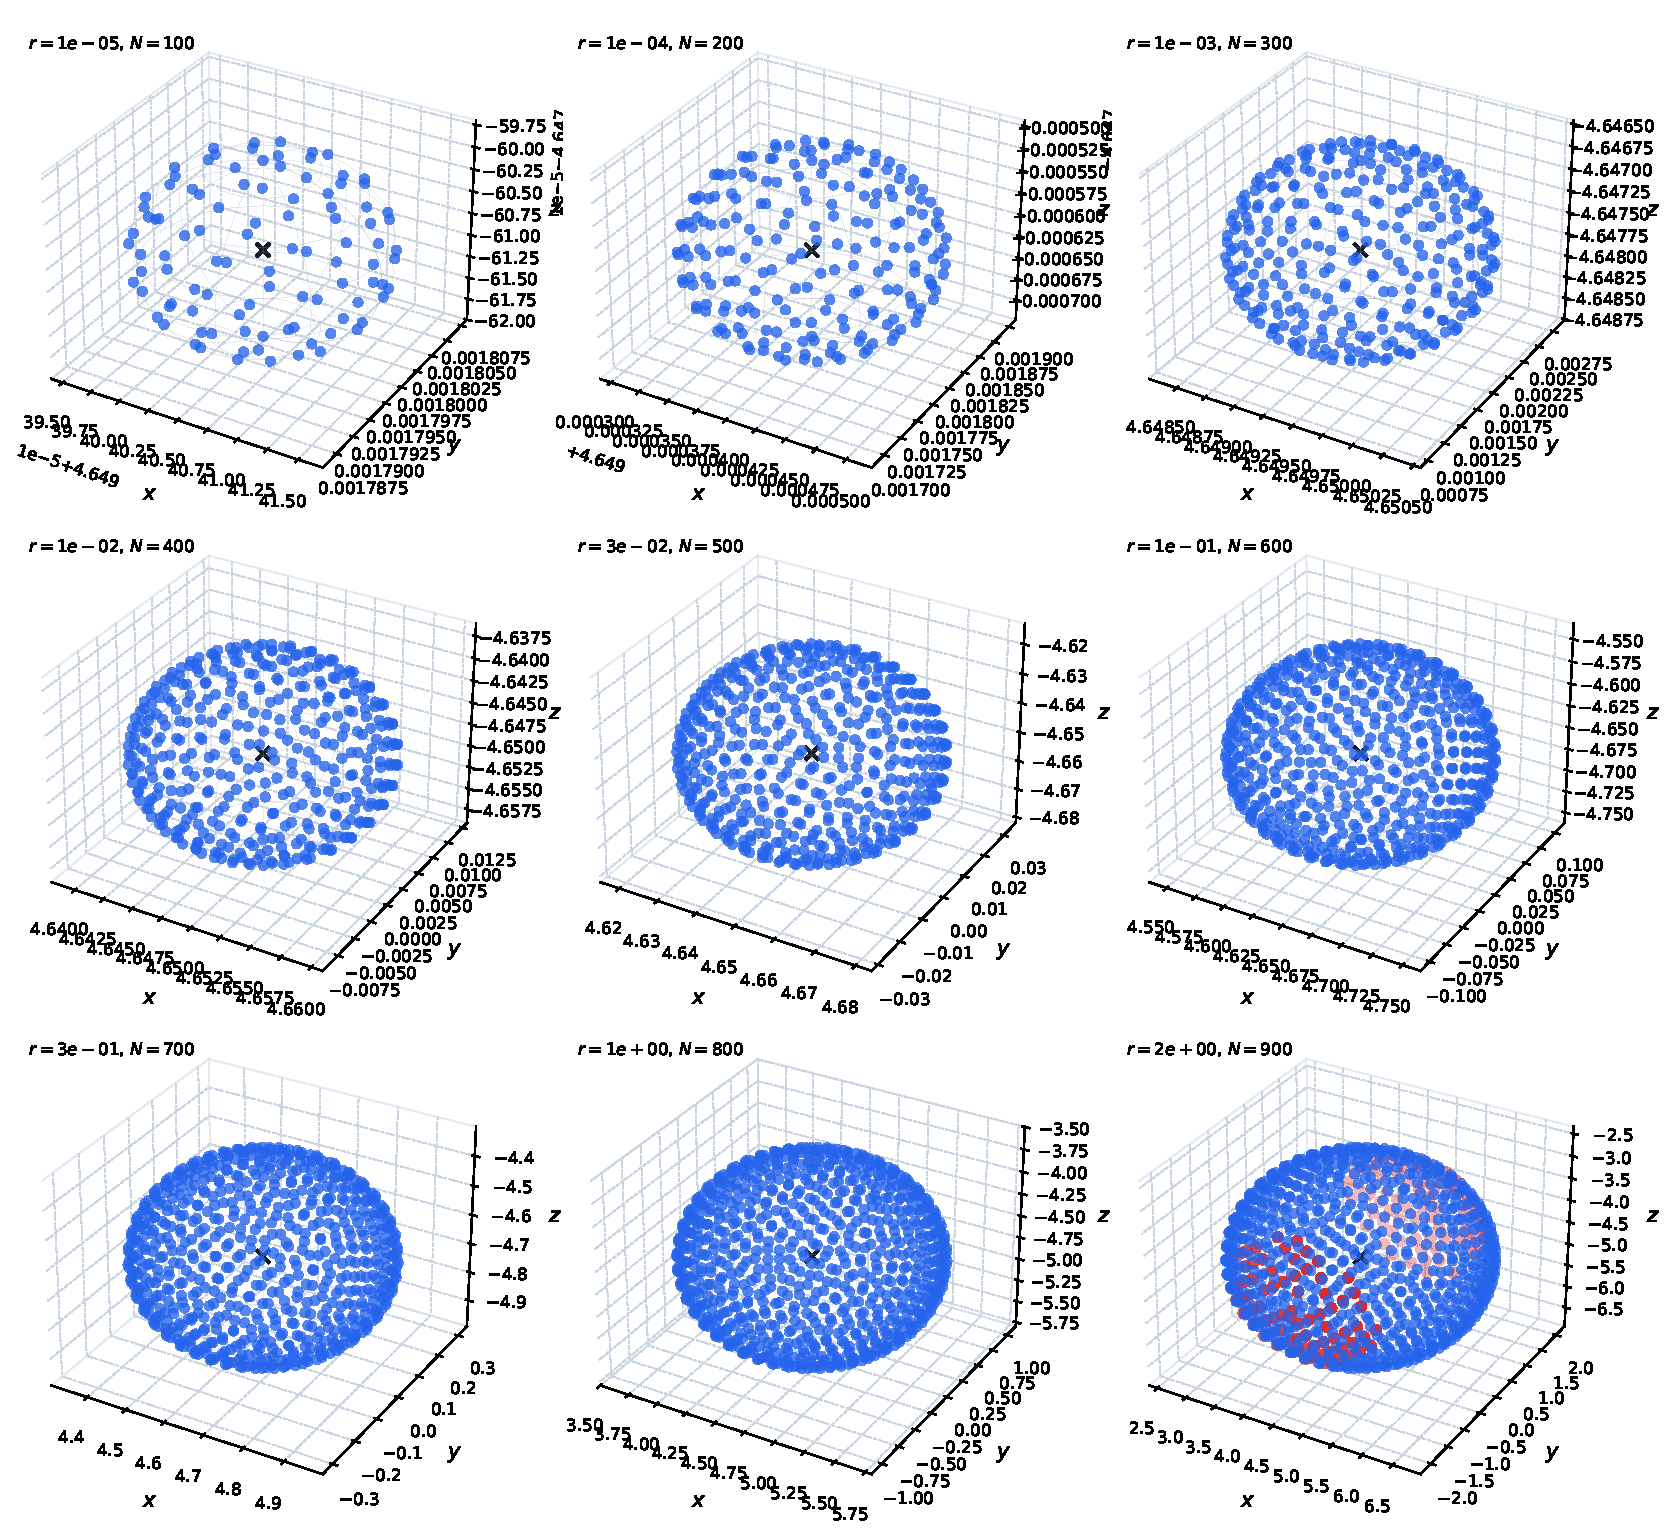
\includegraphics[width=0.94\linewidth,height=0.37\textheight,keepaspectratio]{figures/chua_master/chua_frac_arctan_c590_fig13_Ep_hiddenness_spherical_3d.pdf}\\[-0.25em]
{\footnotesize Chua arctangente c590: sondeos esféricos próximos a \(E_+\).}
\end{center}
\clearpage
\begin{center}
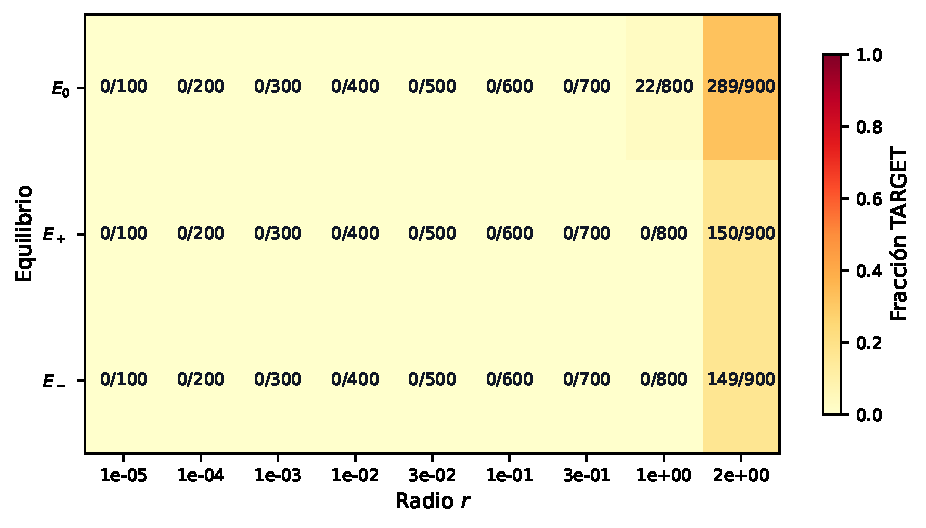
\includegraphics[width=0.94\linewidth,height=0.37\textheight,keepaspectratio]{figures/chua_master/chua_frac_arctan_c590_fig14_hiddenness_contact_heatmap.pdf}\\[-0.25em]
{\footnotesize Chua arctangente c590: frecuencia de contacto por radio y equilibrio.}
\end{center}
\vfill
\begin{center}

\includegraphics[width=0.94\linewidth,height=0.37\textheight,keepaspectratio]{figures/chua_master/chua_frac_ns_biased_fig01a_transfer_real.pdf}\\[-0.25em]
{\footnotesize Chua fraccionario PWL sesgado: parte real de la transferencia.}
\end{center}
\clearpage
\begin{center}

\includegraphics[width=0.94\linewidth,height=0.37\textheight,keepaspectratio]{figures/chua_master/chua_frac_ns_biased_fig01b_transfer_imag.pdf}\\[-0.25em]
{\footnotesize Chua fraccionario PWL sesgado: parte imaginaria de la transferencia.}
\end{center}
\vfill
\begin{center}

\includegraphics[width=0.94\linewidth,height=0.37\textheight,keepaspectratio]{figures/chua_master/chua_frac_ns_biased_fig02_continuation_story.pdf}\\[-0.25em]
{\footnotesize Chua fraccionario PWL sesgado: evolución de la trayectoria durante la continuación.}
\end{center}
\clearpage
\begin{center}
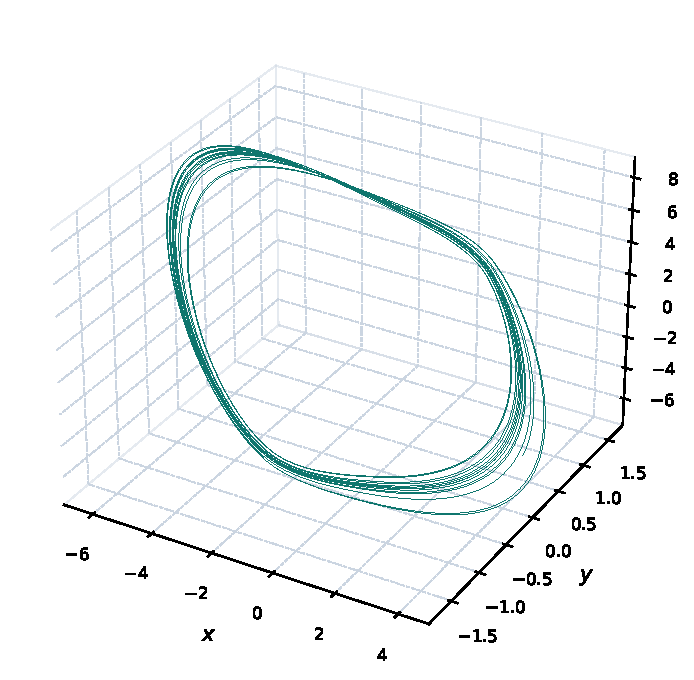
\includegraphics[width=0.94\linewidth,height=0.37\textheight,keepaspectratio]{figures/chua_master/chua_frac_ns_biased_fig03_attractor.pdf}\\[-0.25em]
{\footnotesize Chua fraccionario PWL sesgado: trayectoria candidata en el espacio de estados.}
\end{center}
\vfill
\begin{center}
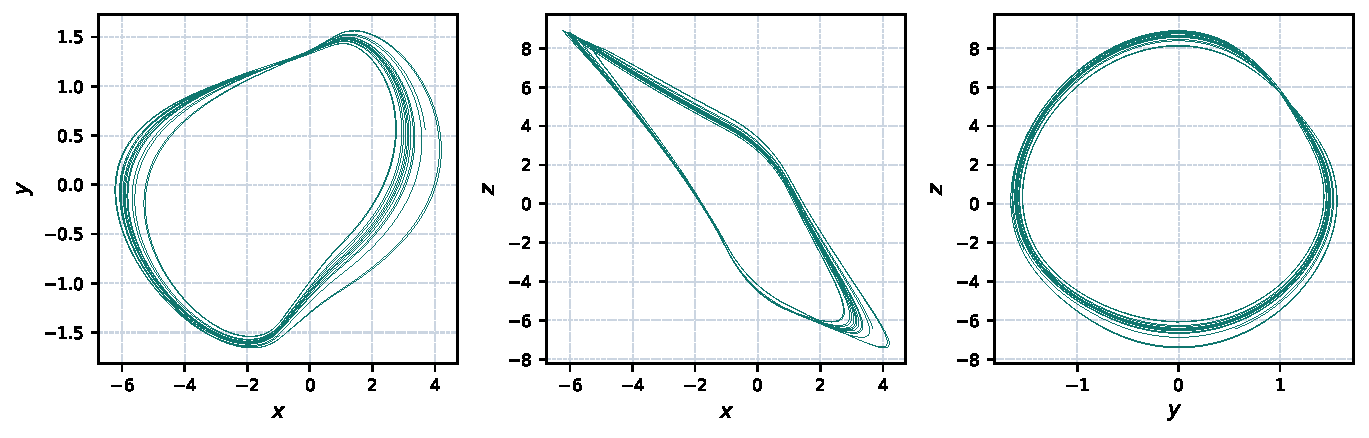
\includegraphics[width=0.94\linewidth,height=0.37\textheight,keepaspectratio]{figures/chua_master/chua_frac_ns_biased_fig04_projections.pdf}\\[-0.25em]
{\footnotesize Chua fraccionario PWL sesgado: proyecciones de la trayectoria candidata.}
\end{center}
\clearpage
\begin{center}
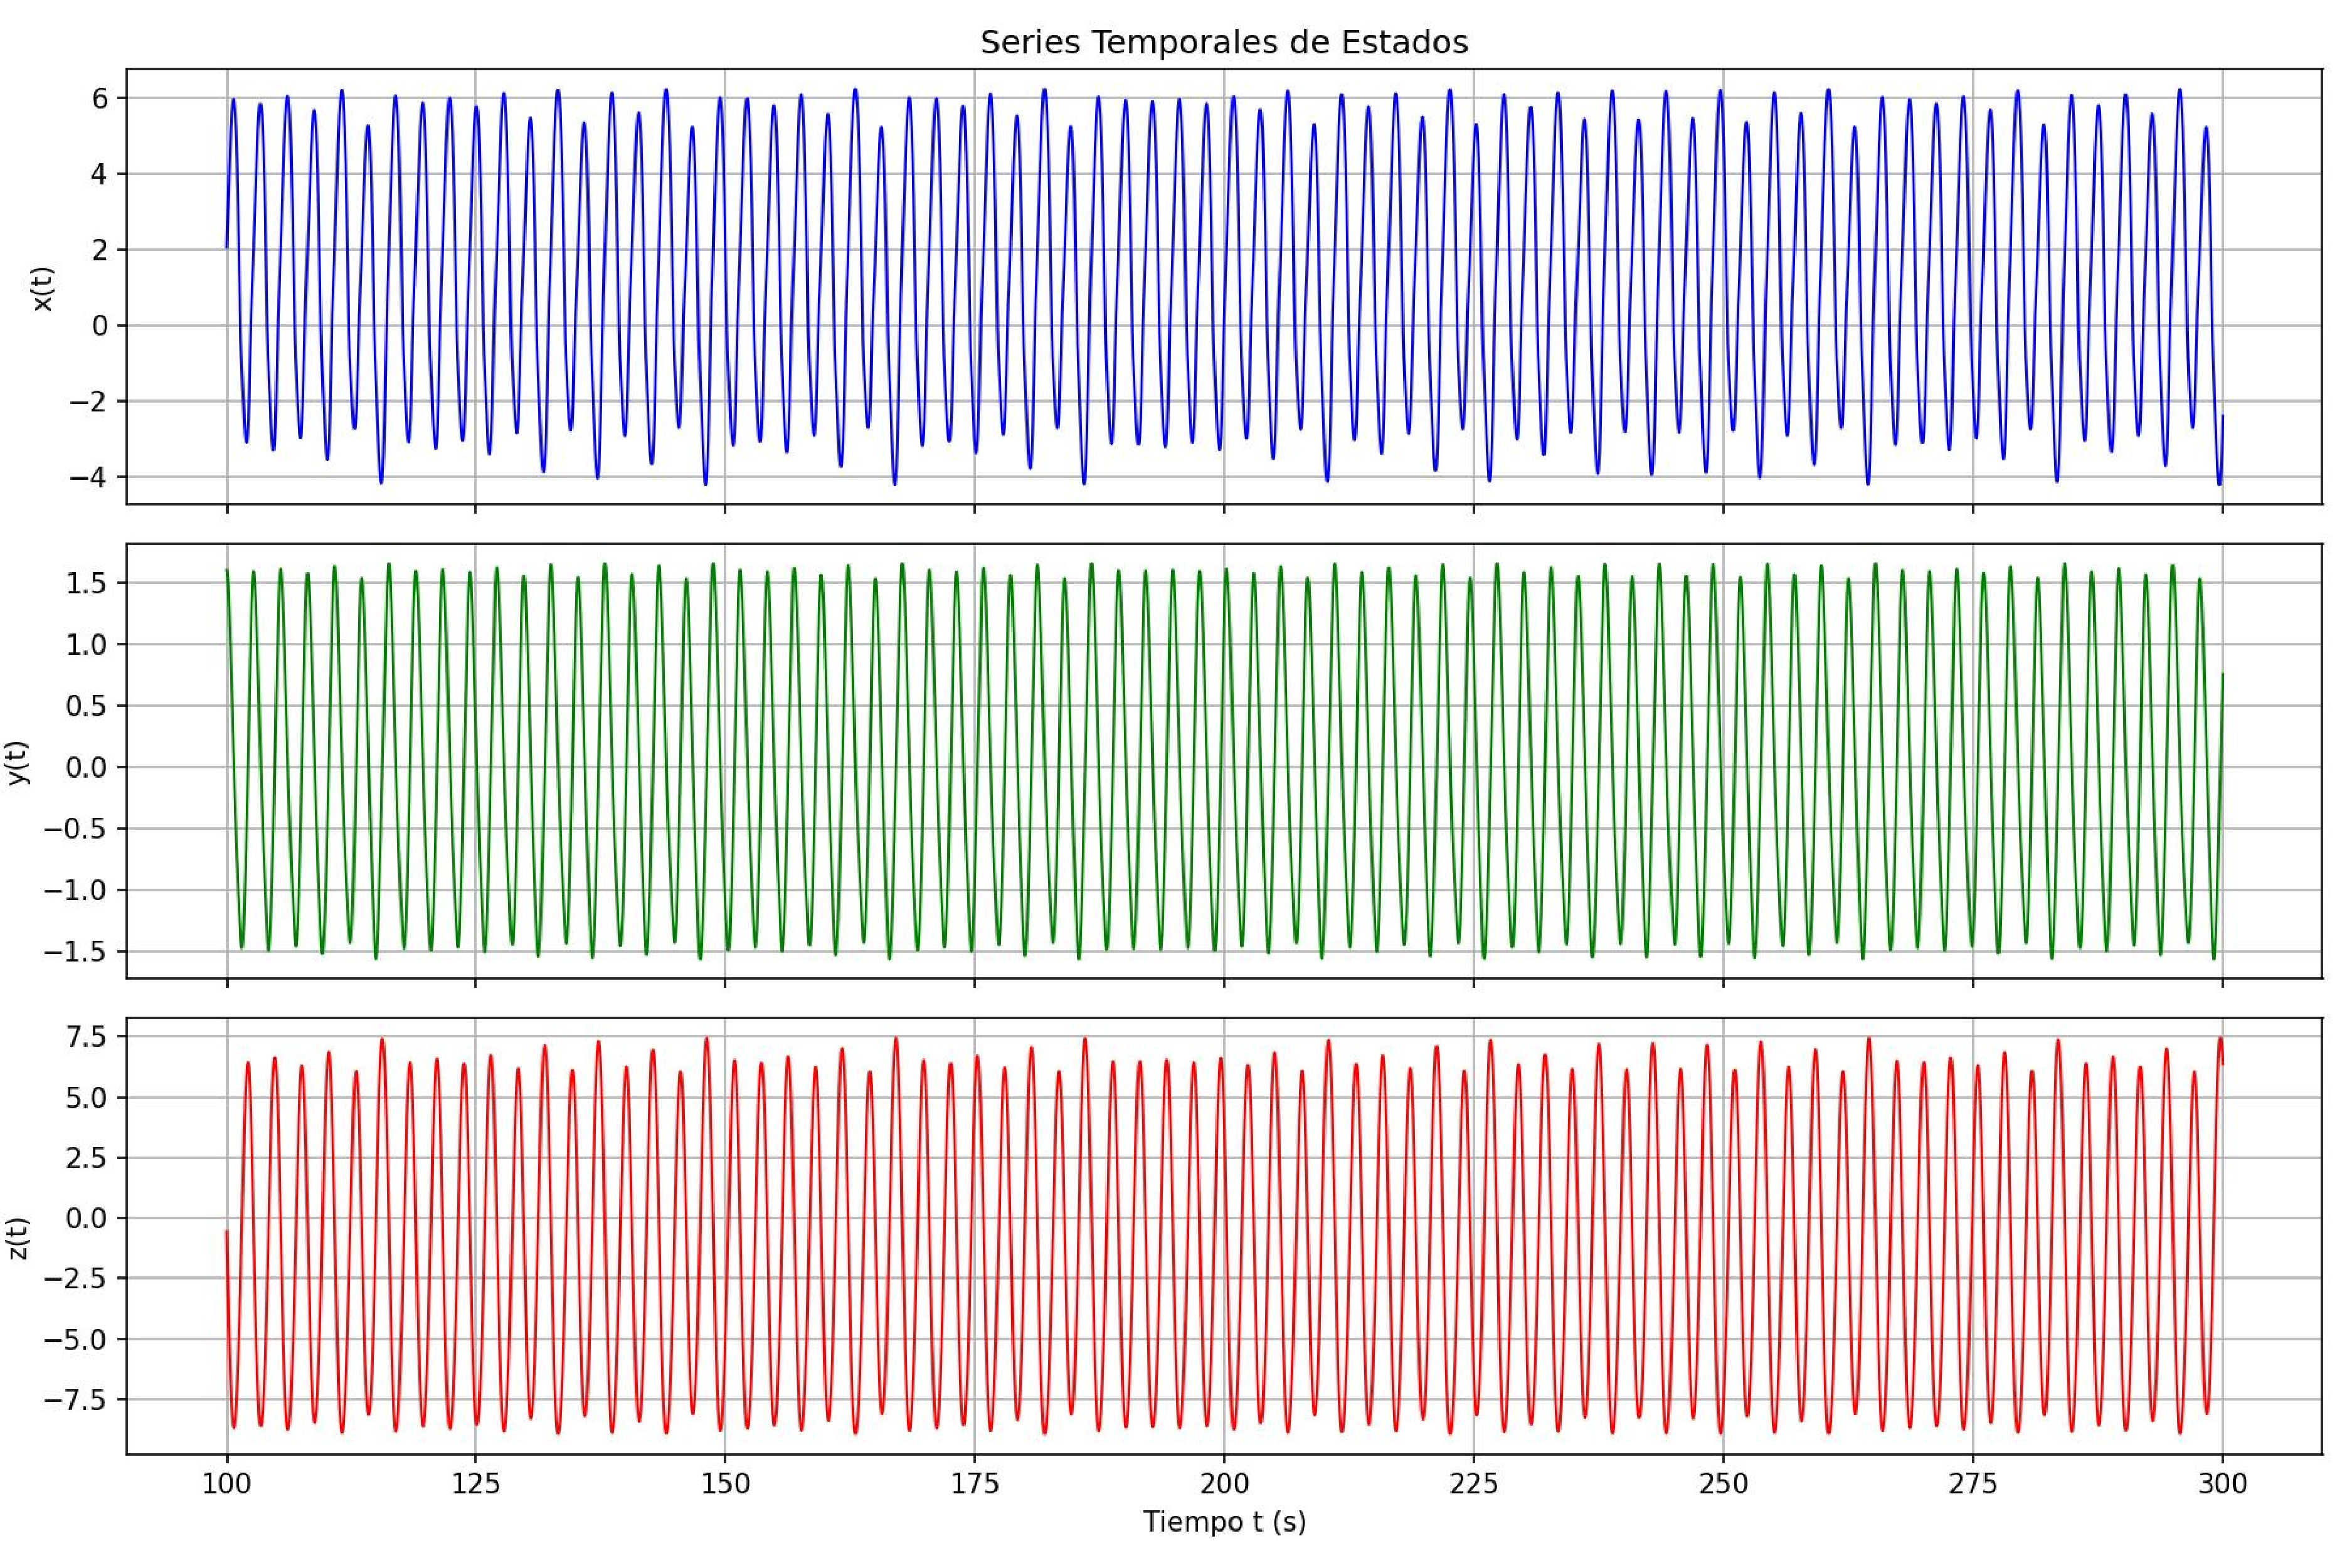
\includegraphics[width=0.94\linewidth,height=0.37\textheight,keepaspectratio]{figures/chua_master/chua_frac_ns_biased_fig04_timeseries.pdf}\\[-0.25em]
{\footnotesize Chua fraccionario PWL sesgado: series temporales.}
\end{center}
\vfill
\begin{center}

\includegraphics[width=0.94\linewidth,height=0.37\textheight,keepaspectratio]{figures/chua_master/chua_frac_ns_biased_fig11_fft.pdf}\\[-0.25em]
{\footnotesize Chua fraccionario PWL sesgado: espectro de amplitud.}
\end{center}
\clearpage
\begin{center}

\includegraphics[width=0.94\linewidth,height=0.37\textheight,keepaspectratio]{figures/chua_master/chua_frac_ns_biased_fig12_lyapunov.pdf}\\[-0.25em]
{\footnotesize Chua fraccionario PWL sesgado: evolución de las estimaciones de Lyapunov.}
\end{center}
\vfill
\begin{center}

\includegraphics[width=0.94\linewidth,height=0.37\textheight,keepaspectratio]{figures/chua_master/chua_frac_ns_biased_fig13_E0_hiddenness_spherical_3d.pdf}\\[-0.25em]
{\footnotesize Chua fraccionario PWL sesgado: sondeos esféricos próximos a \(E_0\).}
\end{center}
\clearpage
\begin{center}

\includegraphics[width=0.94\linewidth,height=0.37\textheight,keepaspectratio]{figures/chua_master/chua_frac_ns_biased_fig13_Em_hiddenness_spherical_3d.pdf}\\[-0.25em]
{\footnotesize Chua fraccionario PWL sesgado: sondeos esféricos próximos a \(E_-\).}
\end{center}
\vfill
\begin{center}

\includegraphics[width=0.94\linewidth,height=0.37\textheight,keepaspectratio]{figures/chua_master/chua_frac_ns_biased_fig13_Ep_hiddenness_spherical_3d.pdf}\\[-0.25em]
{\footnotesize Chua fraccionario PWL sesgado: sondeos esféricos próximos a \(E_+\).}
\end{center}
\clearpage
\begin{center}

\includegraphics[width=0.94\linewidth,height=0.37\textheight,keepaspectratio]{figures/chua_master/chua_frac_ns_biased_fig14_hiddenness_contact_heatmap.pdf}\\[-0.25em]
{\footnotesize Chua fraccionario PWL sesgado: frecuencia de contacto por radio y equilibrio.}
\end{center}
\vfill
\begin{center}
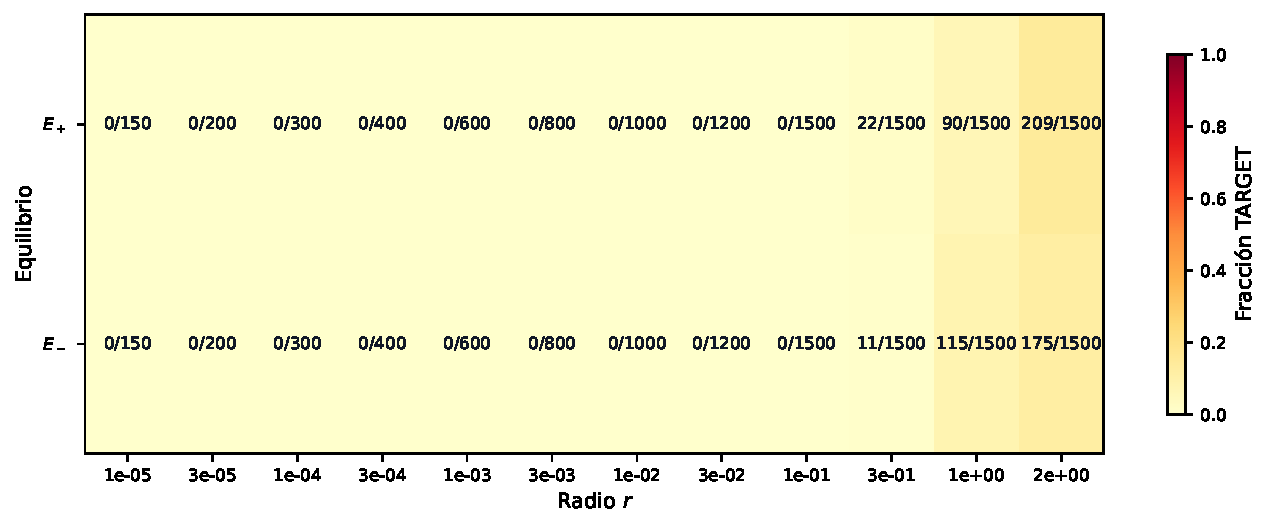
\includegraphics[width=0.94\linewidth,height=0.37\textheight,keepaspectratio]{figures/chua_master/chua_frac_ns_biased_fig15_extended_heatmap.pdf}\\[-0.25em]
{\footnotesize Chua fraccionario PWL sesgado: contactos a radios ampliados.}
\end{center}
\clearpage
\begin{center}

\includegraphics[width=0.94\linewidth,height=0.37\textheight,keepaspectratio]{figures/chua_master/chua_frac_ns_fig01a_transfer_real.pdf}\\[-0.25em]
{\footnotesize Chua fraccionario PWL, control cercano: parte real de la transferencia.}
\end{center}
\vfill
\begin{center}

\includegraphics[width=0.94\linewidth,height=0.37\textheight,keepaspectratio]{figures/chua_master/chua_frac_ns_fig01b_transfer_imag.pdf}\\[-0.25em]
{\footnotesize Chua fraccionario PWL, control cercano: parte imaginaria de la transferencia.}
\end{center}
\clearpage
\begin{center}

\includegraphics[width=0.94\linewidth,height=0.37\textheight,keepaspectratio]{figures/chua_master/chua_frac_ns_fig02_continuation_story.pdf}\\[-0.25em]
{\footnotesize Chua fraccionario PWL, control cercano: evolución de la trayectoria durante la continuación.}
\end{center}
\vfill
\begin{center}

\includegraphics[width=0.94\linewidth,height=0.37\textheight,keepaspectratio]{figures/chua_master/chua_frac_ns_fig03_final_attractor.pdf}\\[-0.25em]
{\footnotesize Chua fraccionario PWL, control cercano: trayectoria final de la continuación.}
\end{center}
\clearpage
\begin{center}

\includegraphics[width=0.94\linewidth,height=0.37\textheight,keepaspectratio]{figures/chua_master/chua_frac_ns_fig03abc_final_attractor_projections.pdf}\\[-0.25em]
{\footnotesize Chua fraccionario PWL, control cercano: proyecciones de la trayectoria final.}
\end{center}
\vfill
\begin{center}

\includegraphics[width=0.94\linewidth,height=0.37\textheight,keepaspectratio]{figures/chua_master/chua_frac_ns_fig04_time_series.pdf}\\[-0.25em]
{\footnotesize Chua fraccionario PWL, control cercano: series temporales.}
\end{center}
\clearpage
\begin{center}

\includegraphics[width=0.94\linewidth,height=0.37\textheight,keepaspectratio]{figures/chua_master/chua_frac_ns_fig11a_fft_x.pdf}\\[-0.25em]
{\footnotesize Chua fraccionario PWL, control cercano: espectro de amplitud de \(x\).}
\end{center}
\vfill
\begin{center}

\includegraphics[width=0.94\linewidth,height=0.37\textheight,keepaspectratio]{figures/chua_master/chua_frac_ns_fig12_lyapunov_two_methods.pdf}\\[-0.25em]
{\footnotesize Chua fraccionario PWL, control cercano: comparación de dos estimaciones de Lyapunov.}
\end{center}
\clearpage
\begin{center}

\includegraphics[width=0.94\linewidth,height=0.37\textheight,keepaspectratio]{figures/chua_master/chua_frac_ns_fig13_E0_hiddenness_spherical_3d.pdf}\\[-0.25em]
{\footnotesize Chua fraccionario PWL, control cercano: sondeos esféricos próximos a \(E_0\).}
\end{center}
\vfill
\begin{center}

\includegraphics[width=0.94\linewidth,height=0.37\textheight,keepaspectratio]{figures/chua_master/chua_frac_ns_fig13_Em_hiddenness_spherical_3d.pdf}\\[-0.25em]
{\footnotesize Chua fraccionario PWL, control cercano: sondeos esféricos próximos a \(E_-\).}
\end{center}
\clearpage
\begin{center}

\includegraphics[width=0.94\linewidth,height=0.37\textheight,keepaspectratio]{figures/chua_master/chua_frac_ns_fig13_Ep_hiddenness_spherical_3d.pdf}\\[-0.25em]
{\footnotesize Chua fraccionario PWL, control cercano: sondeos esféricos próximos a \(E_+\).}
\end{center}
\vfill
\begin{center}

\includegraphics[width=0.94\linewidth,height=0.37\textheight,keepaspectratio]{figures/chua_master/chua_frac_ns_fig14_hiddenness_contact_heatmap.pdf}\\[-0.25em]
{\footnotesize Chua fraccionario PWL, control cercano: frecuencia de contacto por radio y equilibrio.}
\end{center}
\clearpage
\begin{center}
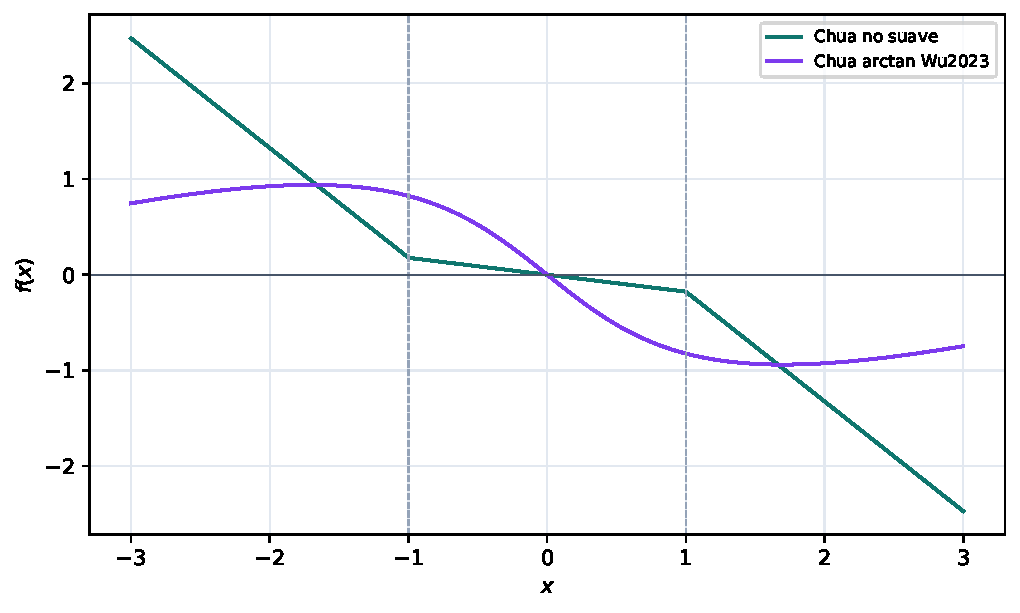
\includegraphics[width=0.94\linewidth,height=0.37\textheight,keepaspectratio]{figures/chua_master/chua_nonlinearity_piecewise_vs_arctan.pdf}\\[-0.25em]
{\footnotesize Comparación de las no linealidades PWL y arctangente.}
\end{center}
\vfill
\begin{center}
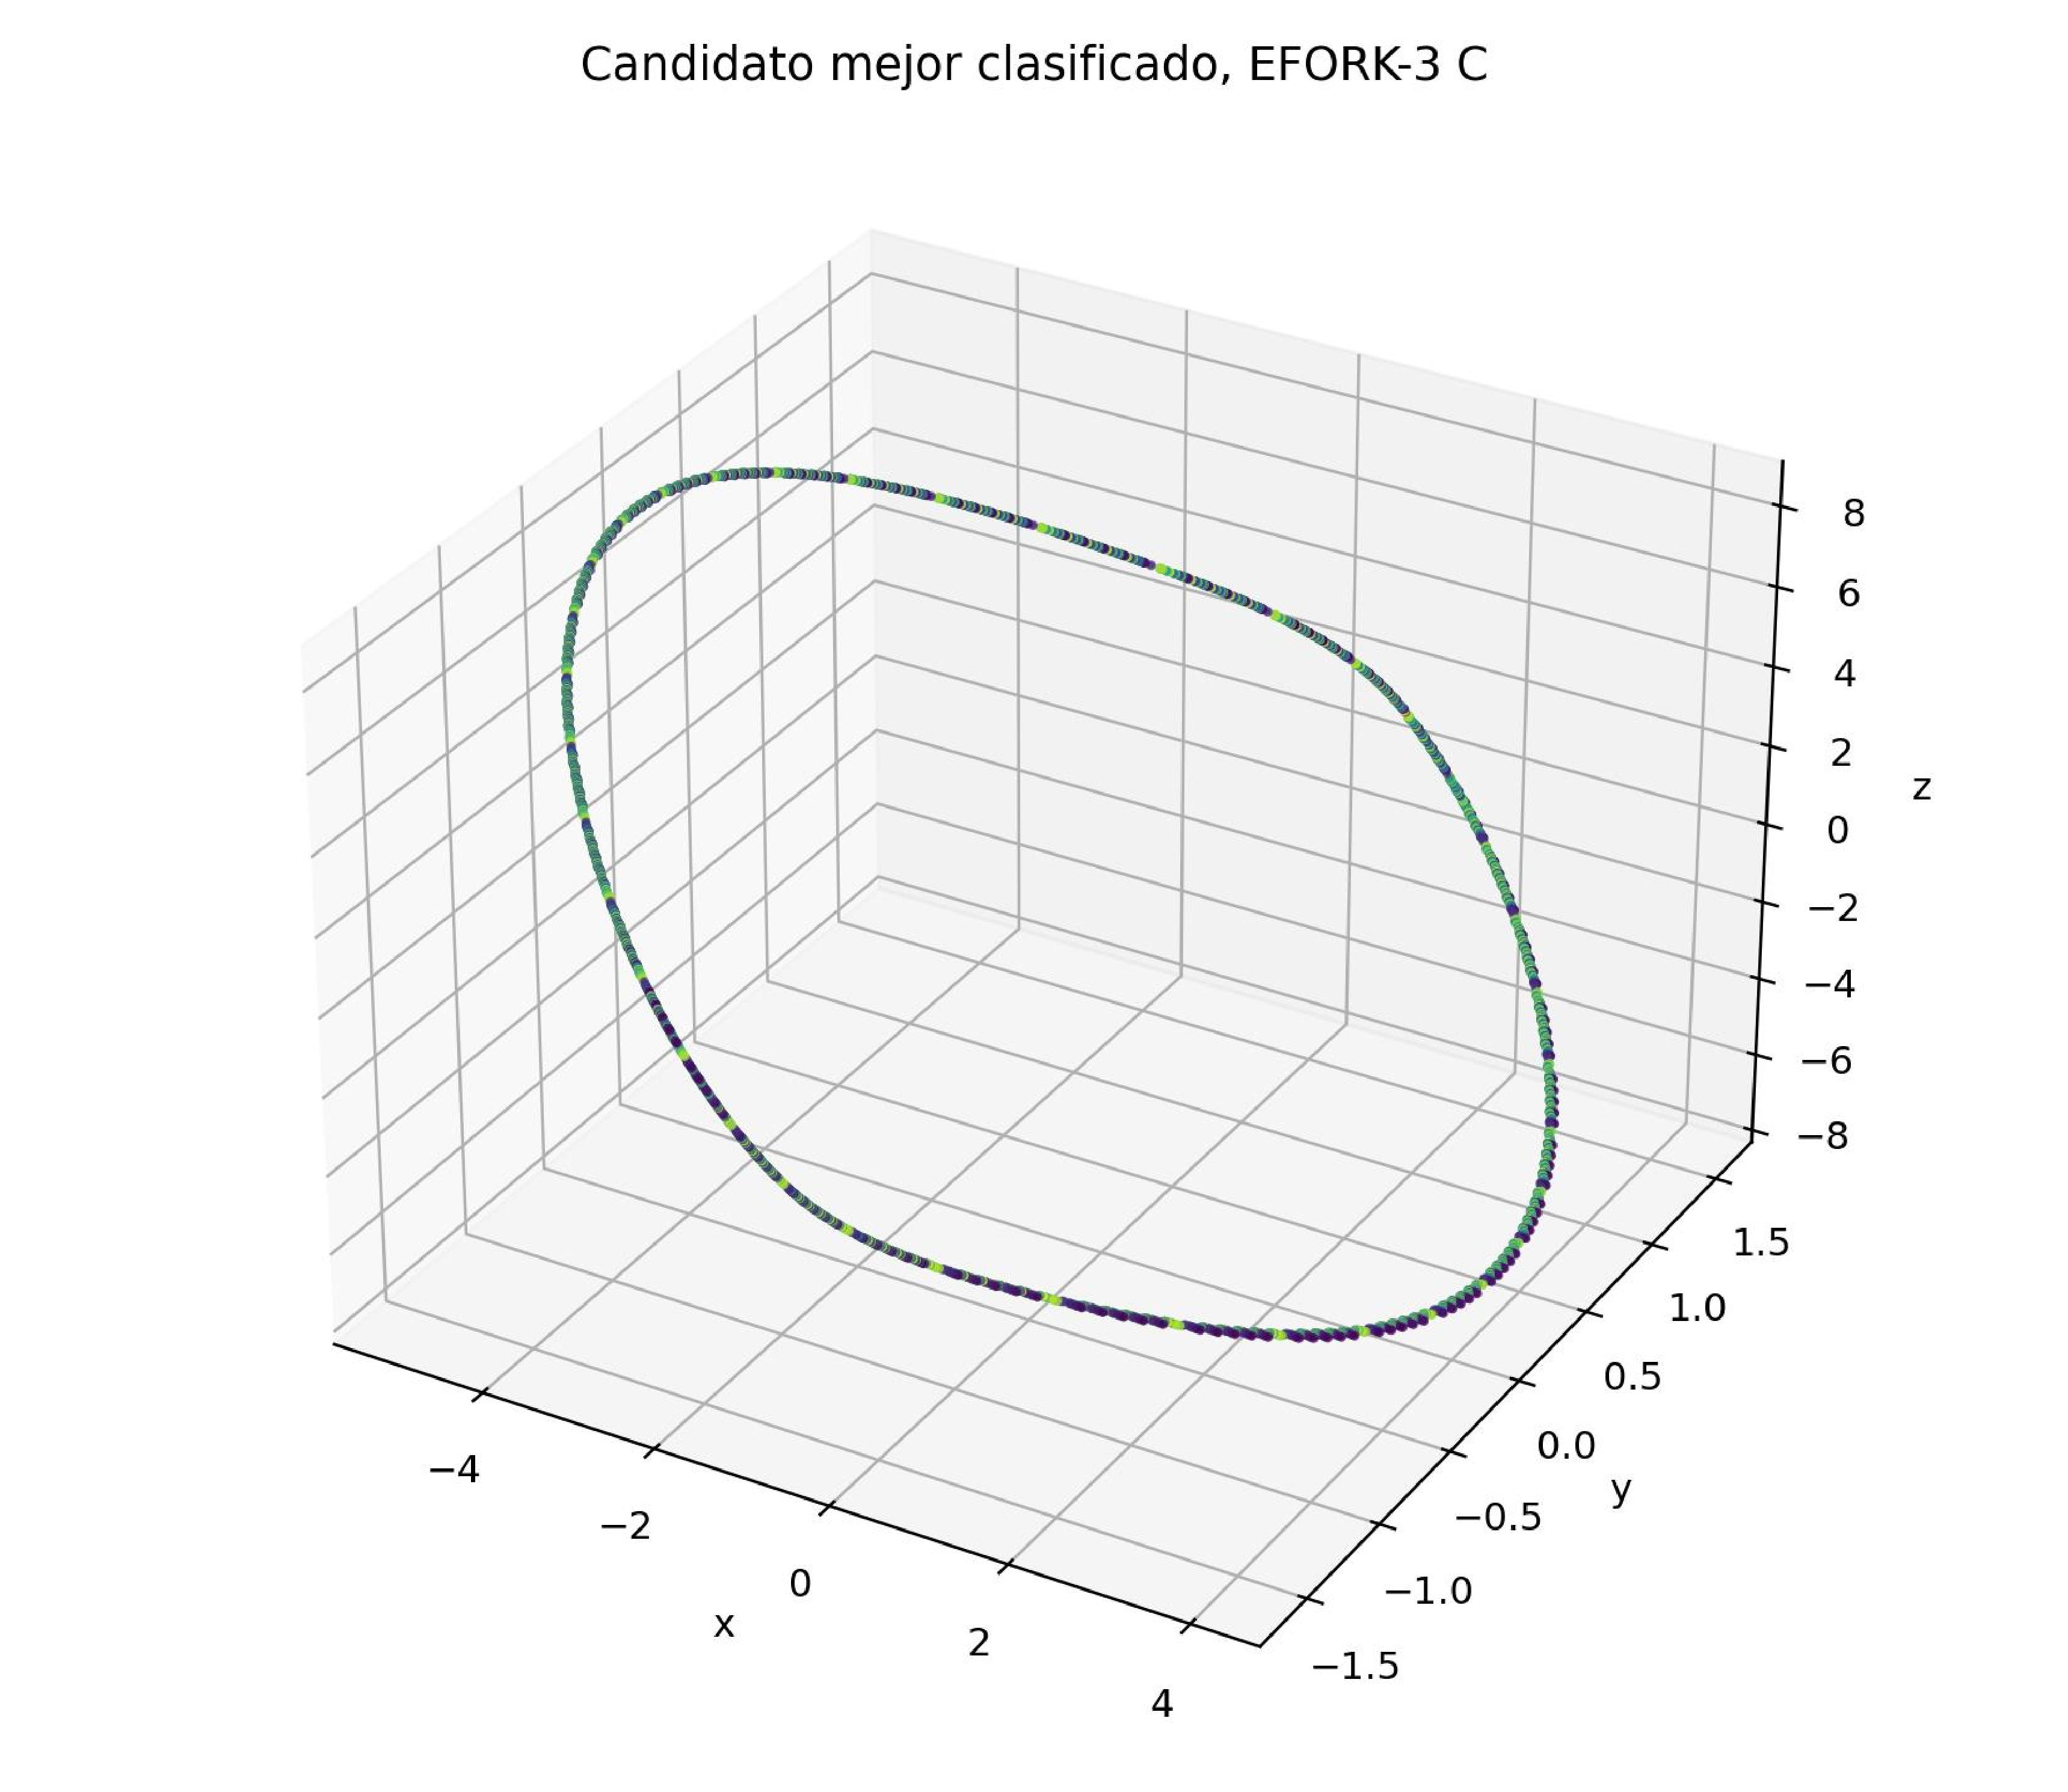
\includegraphics[width=0.94\linewidth,height=0.37\textheight,keepaspectratio]{figures/chua_master/danca_frac_phase_3d.pdf}\\[-0.25em]
{\footnotesize Chua fraccionario con parámetros de Danca: trayectoria en el espacio de estados.}
\end{center}
\clearpage
\begin{center}
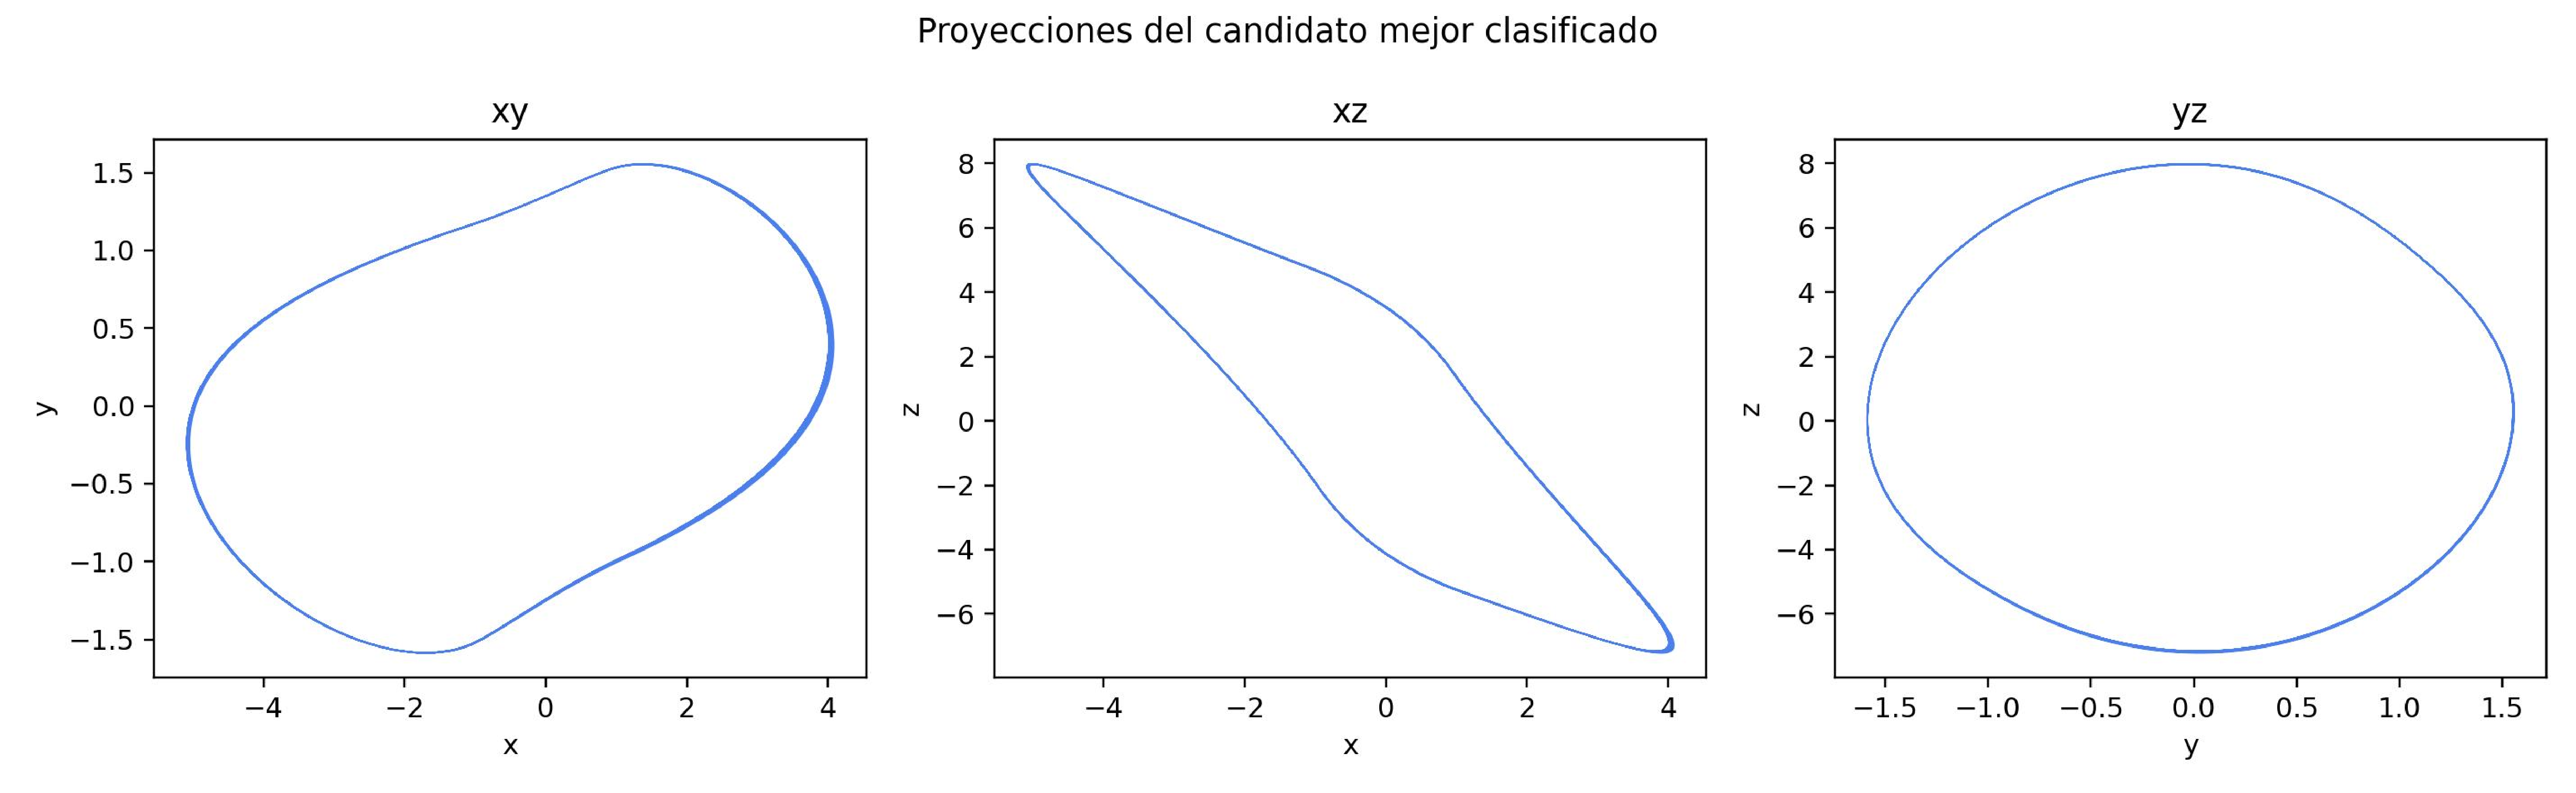
\includegraphics[width=0.94\linewidth,height=0.37\textheight,keepaspectratio]{figures/chua_master/danca_frac_projections.pdf}\\[-0.25em]
{\footnotesize Chua fraccionario con parámetros de Danca: proyecciones de la trayectoria.}
\end{center}
\vfill
\begin{center}
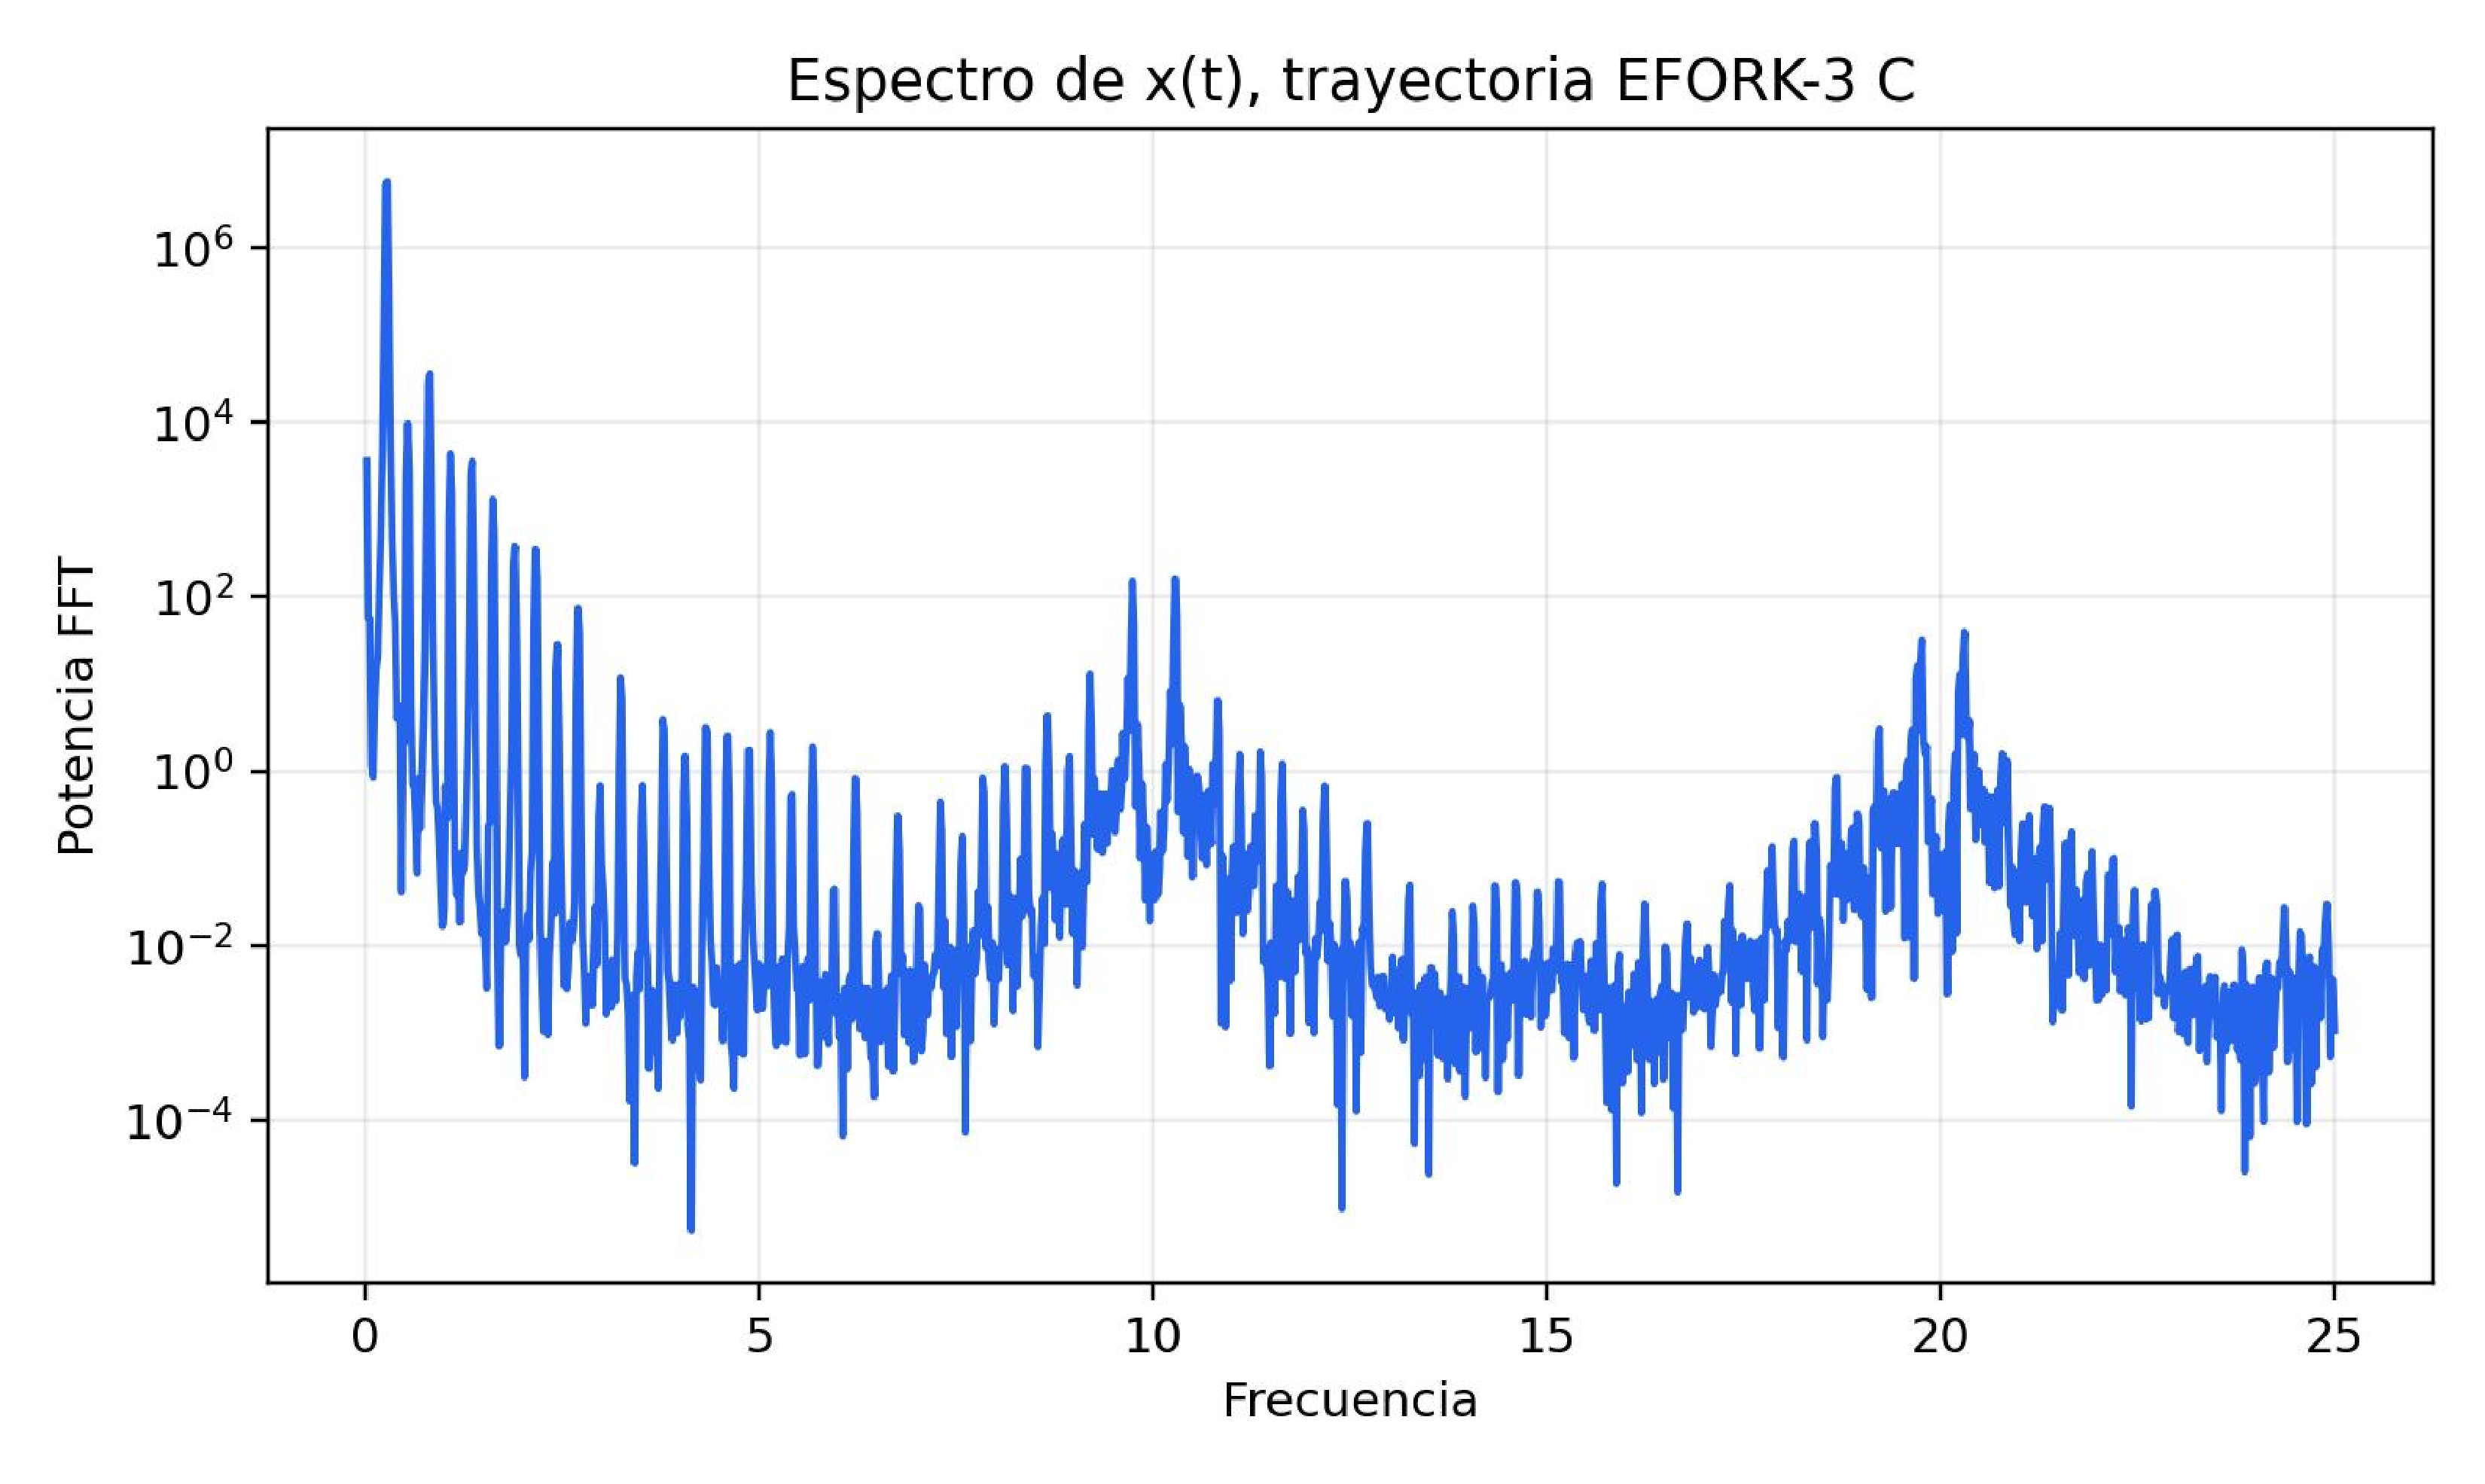
\includegraphics[width=0.94\linewidth,height=0.37\textheight,keepaspectratio]{figures/chua_master/danca_frac_spectrum_x.pdf}\\[-0.25em]
{\footnotesize Chua fraccionario con parámetros de Danca: espectro de la componente \(x\).}
\end{center}
\clearpage
\begin{center}
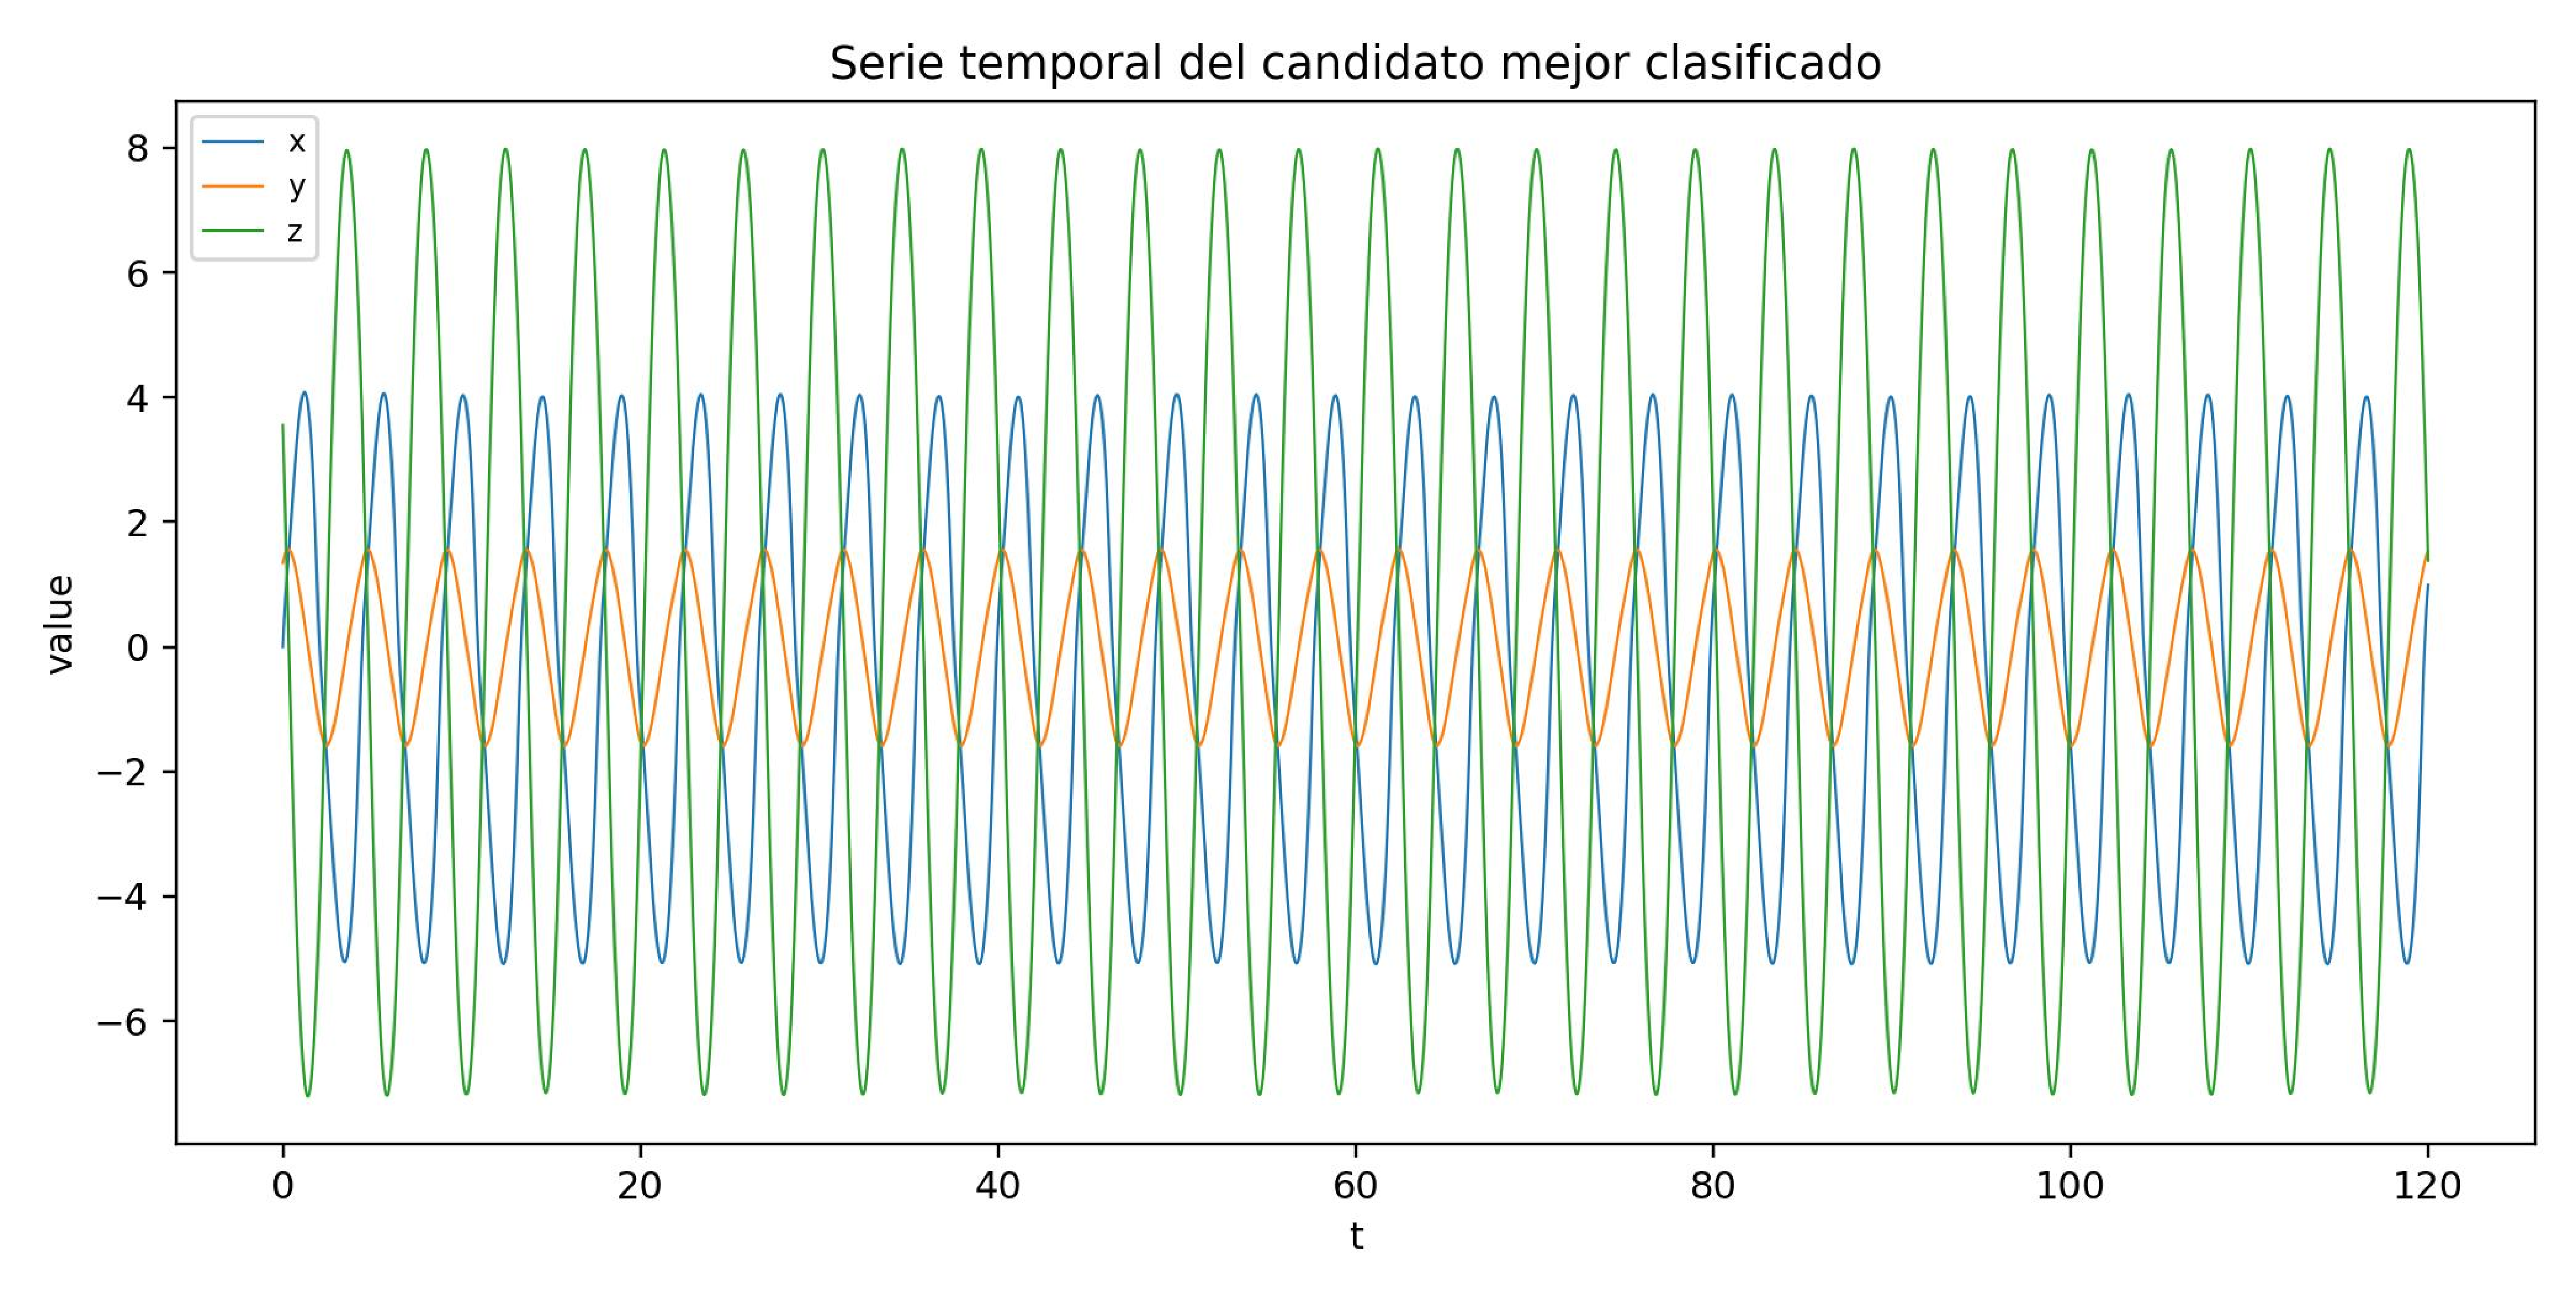
\includegraphics[width=0.94\linewidth,height=0.37\textheight,keepaspectratio]{figures/chua_master/danca_frac_time_series.pdf}\\[-0.25em]
{\footnotesize Chua fraccionario con parámetros de Danca: series temporales.}
\end{center}
\vfill
\begin{center}

\includegraphics[width=0.94\linewidth,height=0.37\textheight,keepaspectratio]{figures/chua_master/fig01_nyquist_df.pdf}\\[-0.25em]
{\footnotesize Chua entero: diagrama de Nyquist y función descriptiva.}
\end{center}
\clearpage
\begin{center}
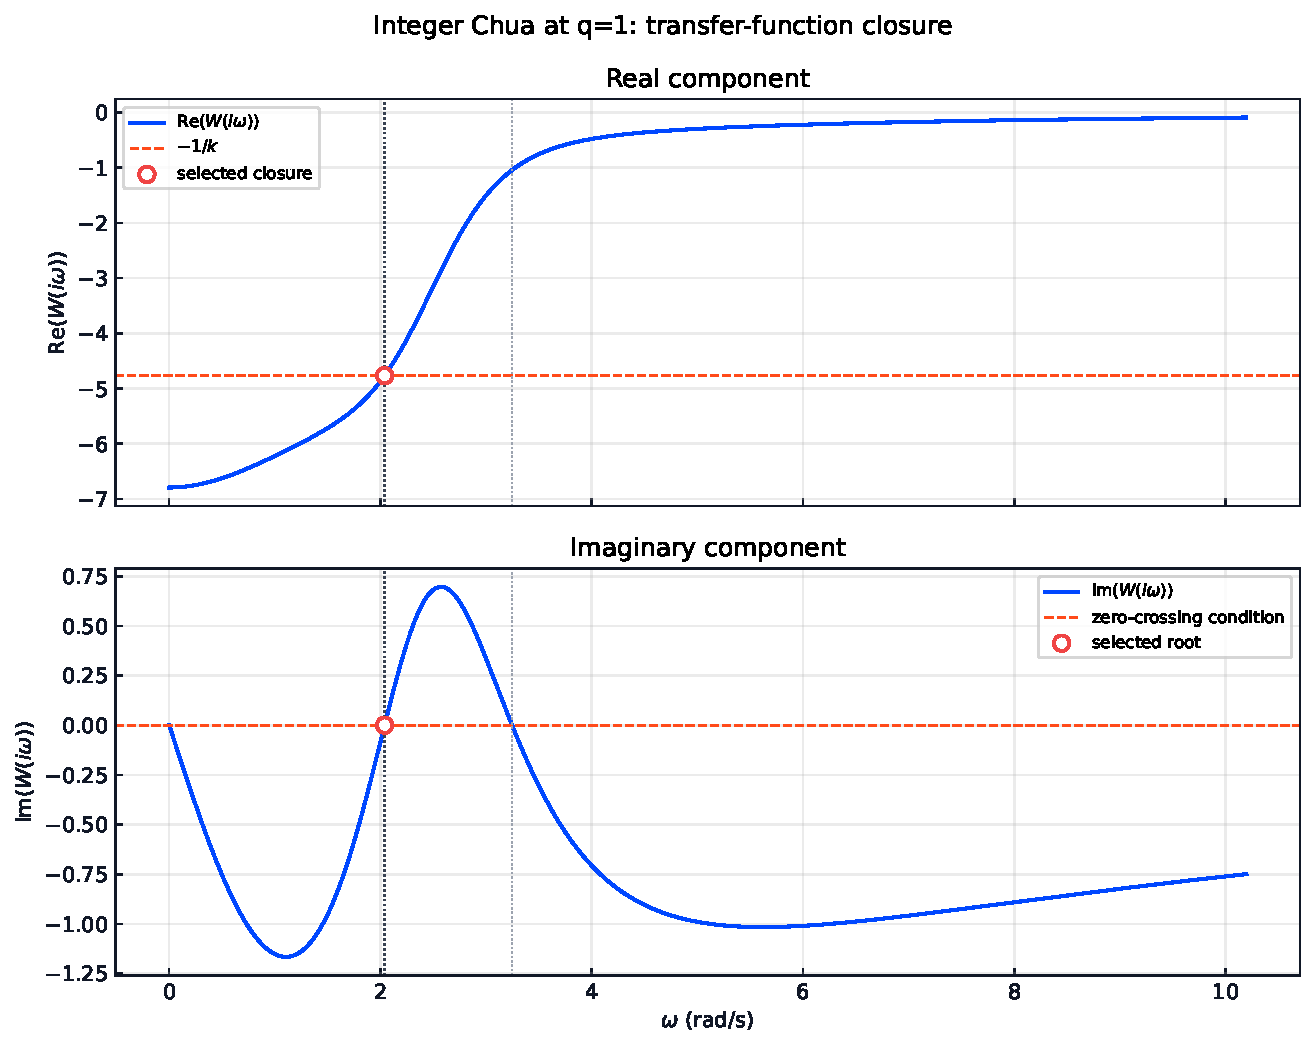
\includegraphics[width=0.94\linewidth,height=0.37\textheight,keepaspectratio]{figures/chua_master/fig01c_transfer_real_imag.pdf}\\[-0.25em]
{\footnotesize Chua entero: partes real e imaginaria de la transferencia.}
\end{center}
\vfill
\begin{center}
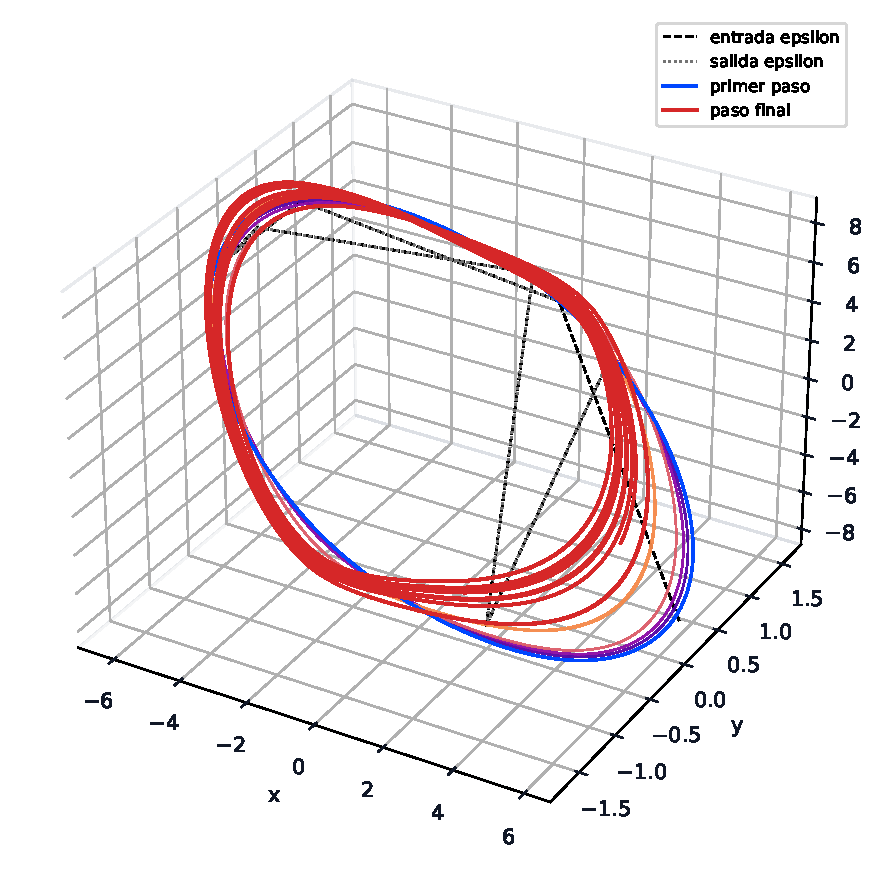
\includegraphics[width=0.94\linewidth,height=0.37\textheight,keepaspectratio]{figures/chua_master/fig02d_continuation_story.pdf}\\[-0.25em]
{\footnotesize Chua entero: evolución de la trayectoria durante la continuación.}
\end{center}
\clearpage
\begin{center}

\includegraphics[width=0.94\linewidth,height=0.37\textheight,keepaspectratio]{figures/chua_master/fig03_final_attractor.pdf}\\[-0.25em]
{\footnotesize Chua entero: trayectoria final de la continuación.}
\end{center}
\vfill
\begin{center}

\includegraphics[width=0.94\linewidth,height=0.37\textheight,keepaspectratio]{figures/chua_master/fig05b_hiddenness_overview.pdf}\\[-0.25em]
{\footnotesize Chua entero: destinos de los sondeos próximos a los equilibrios.}
\end{center}
\clearpage
\begin{center}
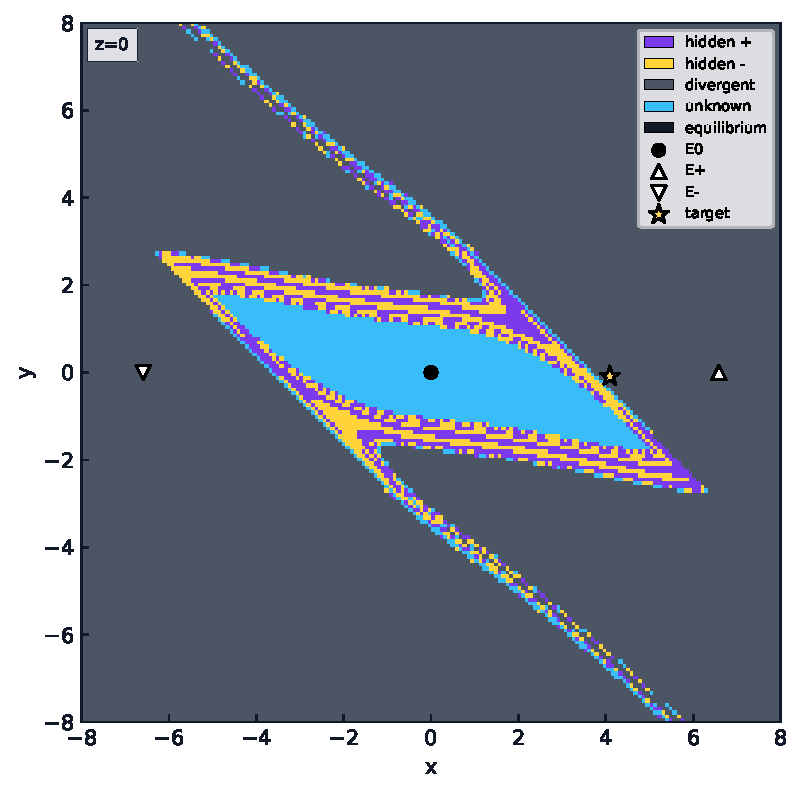
\includegraphics[width=0.94\linewidth,height=0.37\textheight,keepaspectratio]{figures/chua_master/fig06a_basin_overlay_z0.pdf}\\[-0.25em]
{\footnotesize Chua entero: regiones de destino sobre el plano \(z=0\).}
\end{center}
\vfill
\begin{center}
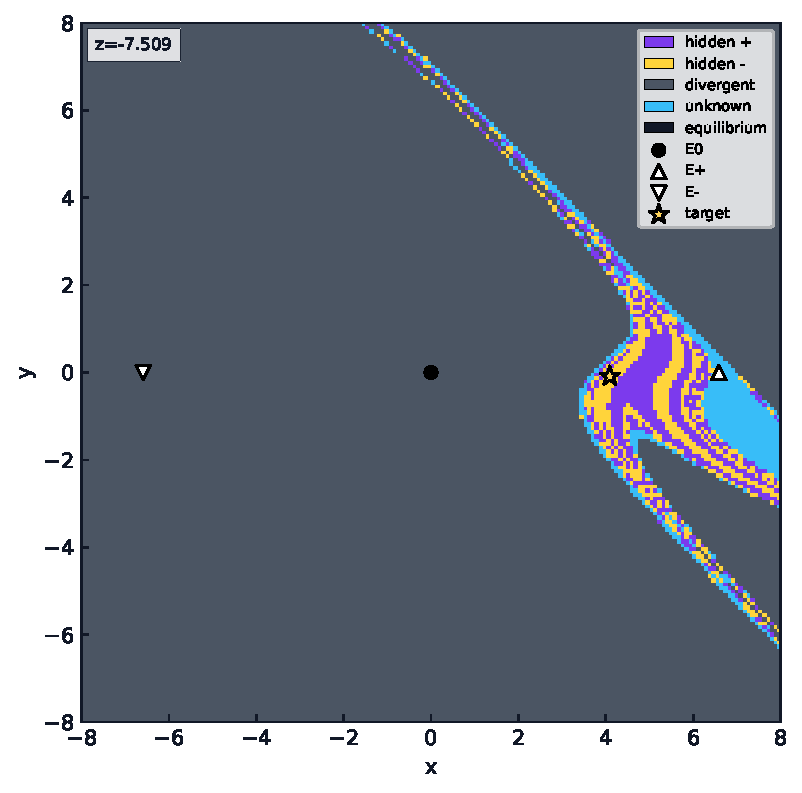
\includegraphics[width=0.94\linewidth,height=0.37\textheight,keepaspectratio]{figures/chua_master/fig06b_basin_overlay_zfinal.pdf}\\[-0.25em]
{\footnotesize Chua entero: regiones de destino sobre un plano transversal a la trayectoria final.}
\end{center}
\clearpage
\begin{center}
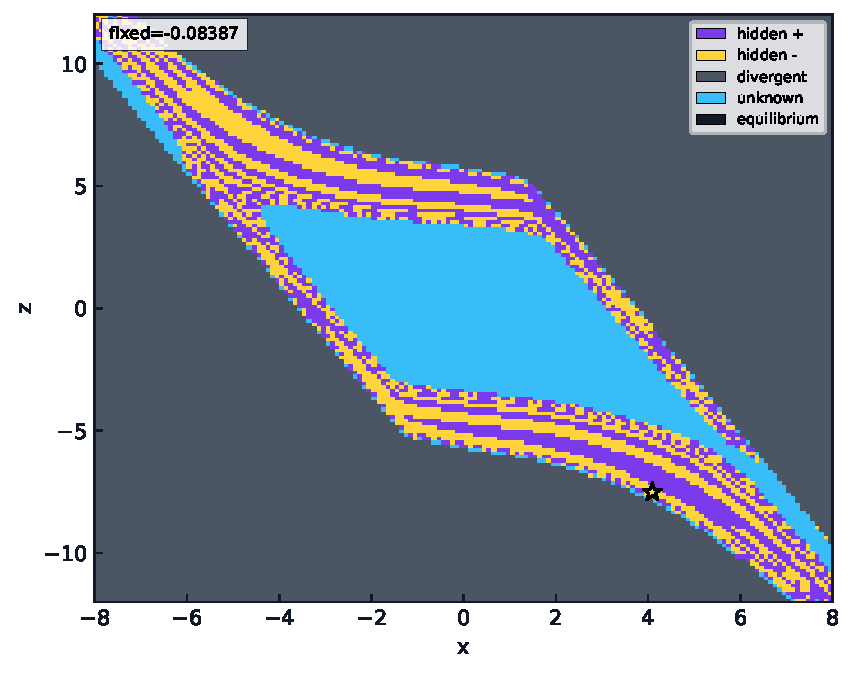
\includegraphics[width=0.94\linewidth,height=0.37\textheight,keepaspectratio]{figures/chua_master/fig10b_basin_xz_final_state.pdf}\\[-0.25em]
{\footnotesize Chua entero: regiones de destino en un corte \(xz\).}
\end{center}
\vfill
\begin{center}
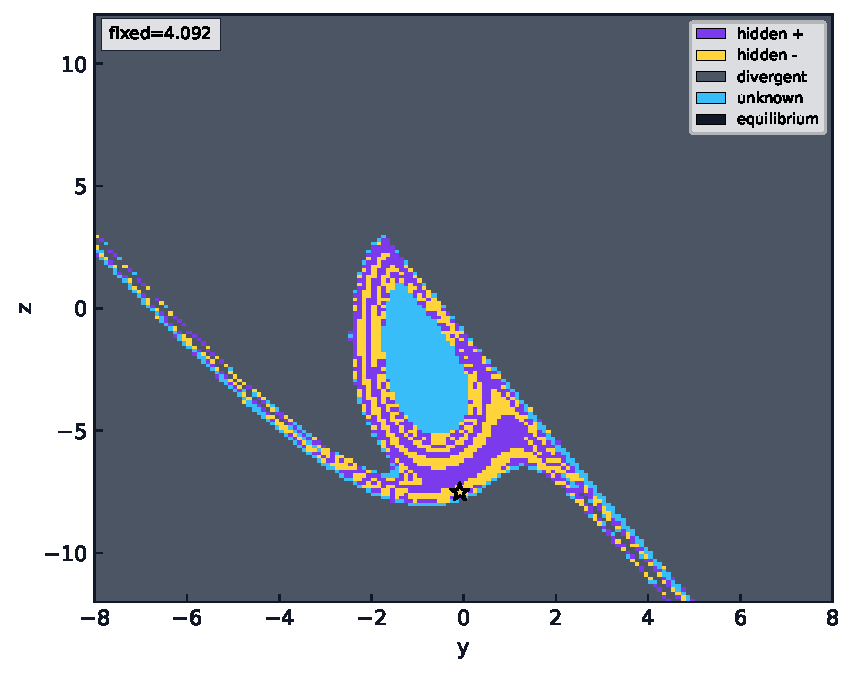
\includegraphics[width=0.94\linewidth,height=0.37\textheight,keepaspectratio]{figures/chua_master/fig10c_basin_yz_final_state.pdf}\\[-0.25em]
{\footnotesize Chua entero: regiones de destino en un corte \(yz\).}
\end{center}
\clearpage
\begin{center}

\includegraphics[width=0.94\linewidth,height=0.37\textheight,keepaspectratio]{figures/chua_master/fig11a_fft_x.pdf}\\[-0.25em]
{\footnotesize Chua entero: espectro de amplitud de \(x\).}
\end{center}
\vfill
\begin{center}
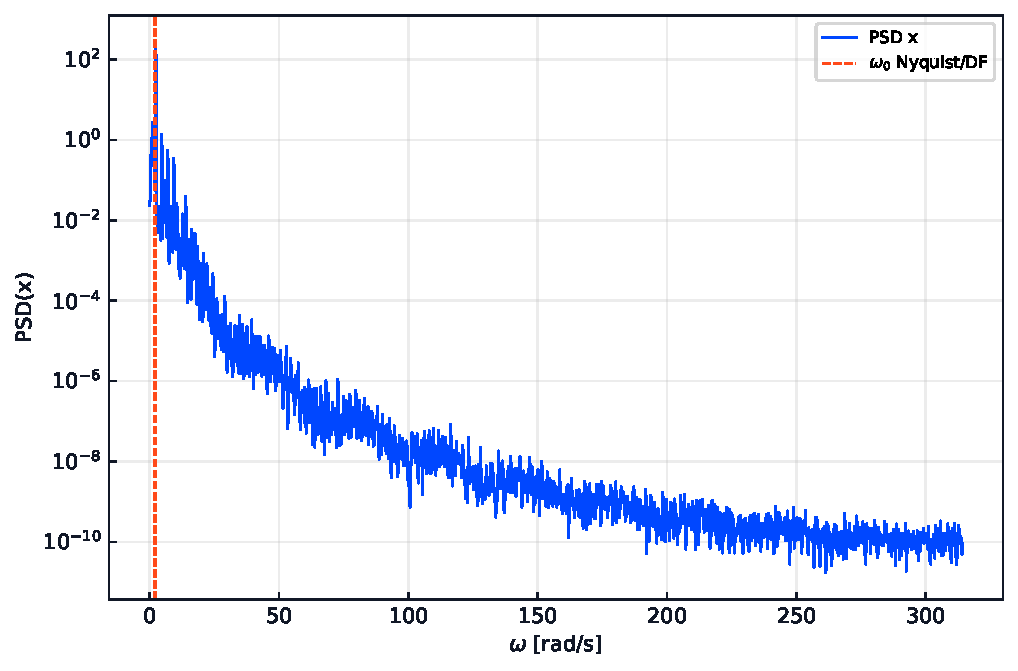
\includegraphics[width=0.94\linewidth,height=0.37\textheight,keepaspectratio]{figures/chua_master/fig11d_psd_x.pdf}\\[-0.25em]
{\footnotesize Chua entero: densidad espectral de potencia de \(x\).}
\end{center}
\clearpage
\begin{center}
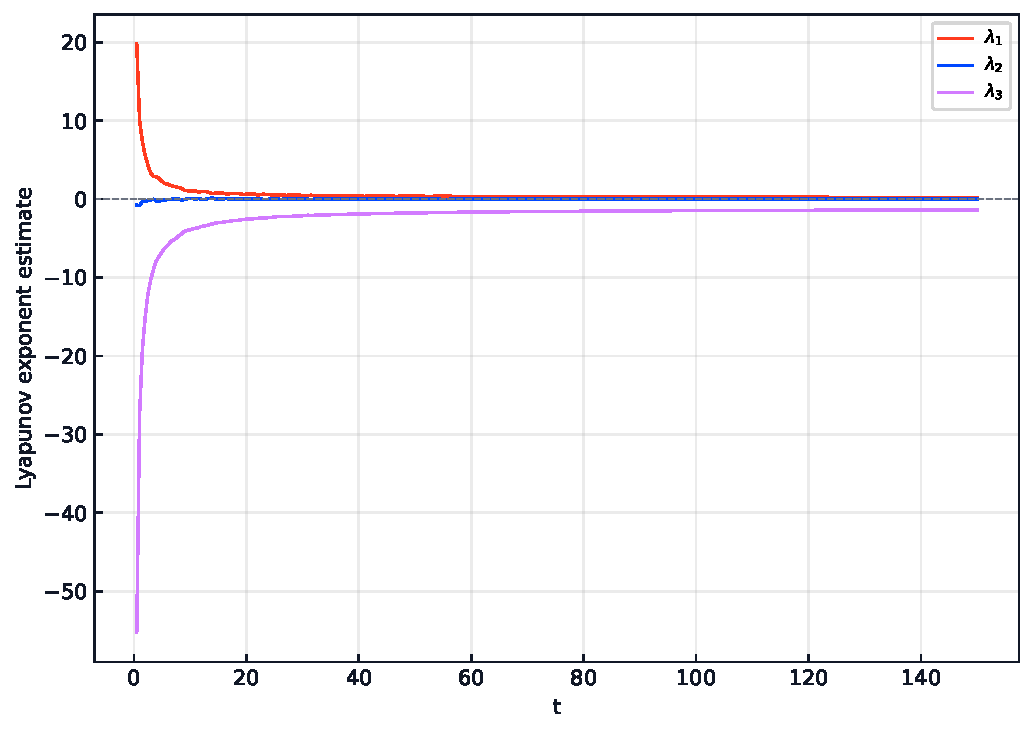
\includegraphics[width=0.94\linewidth,height=0.37\textheight,keepaspectratio]{figures/chua_master/fig13_lyapunov_convergence.pdf}\\[-0.25em]
{\footnotesize Chua entero: evolución de las estimaciones de Lyapunov.}
\end{center}
\vfill
\begin{center}
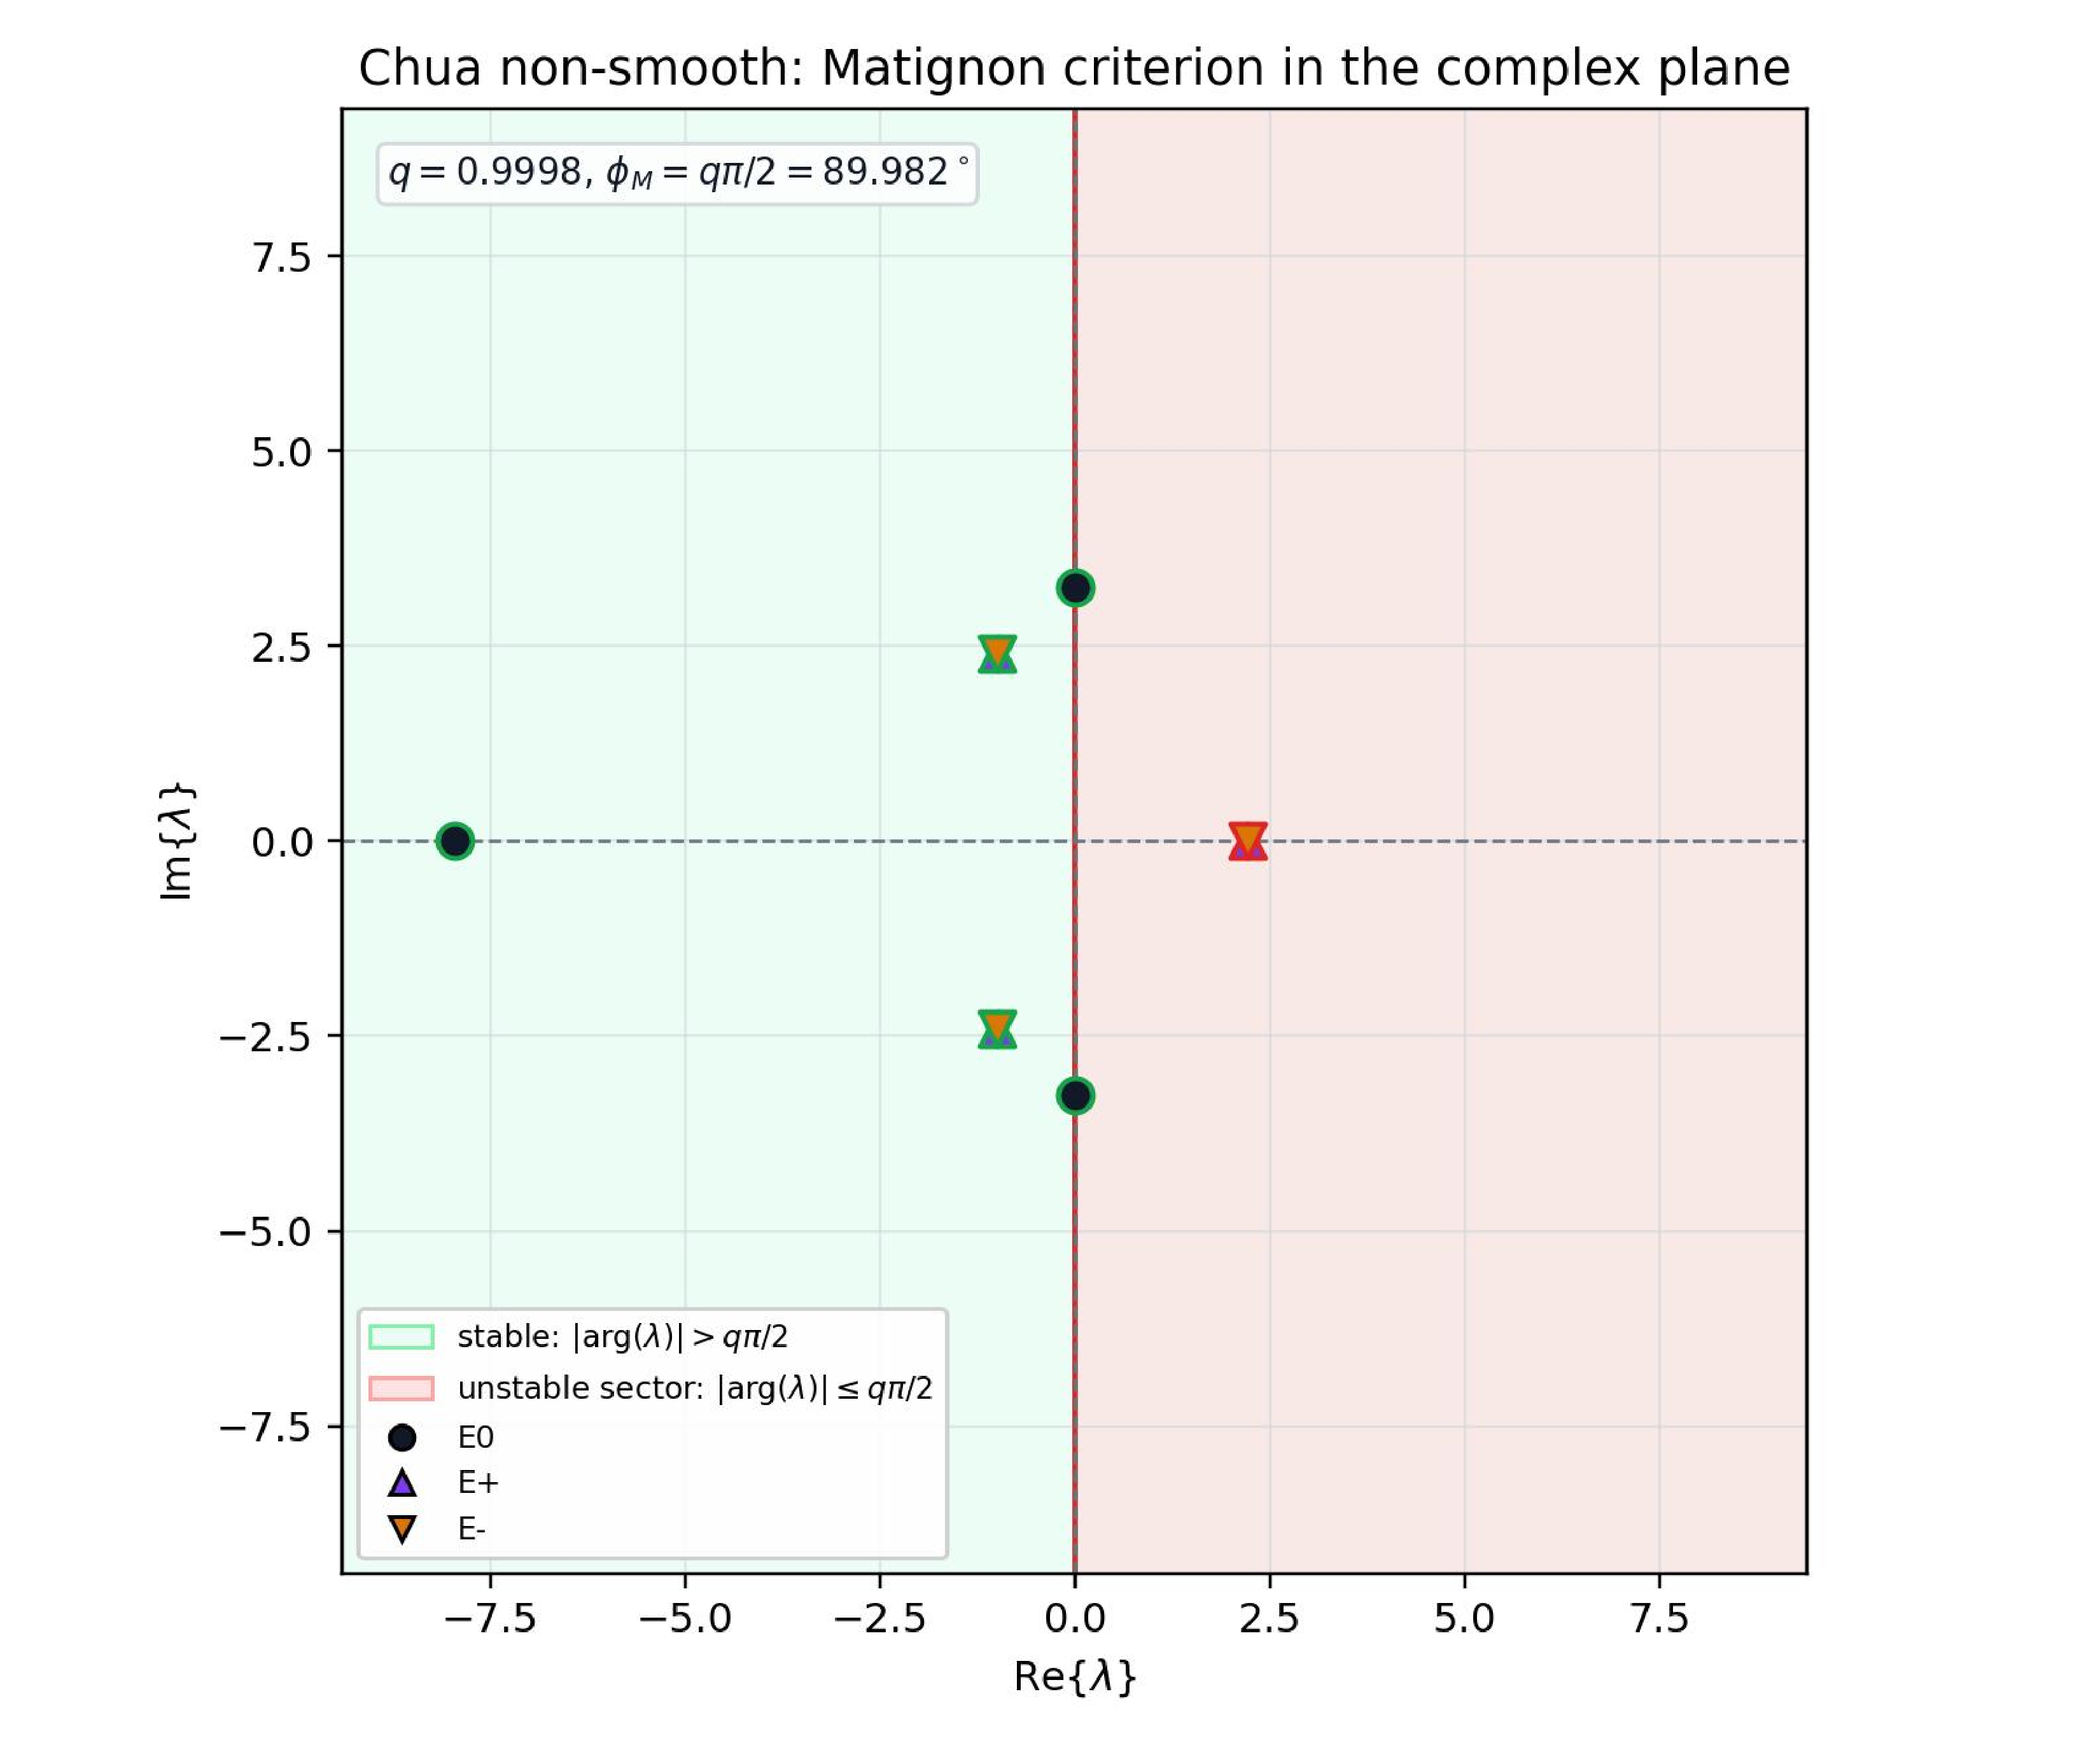
\includegraphics[width=0.94\linewidth,height=0.37\textheight,keepaspectratio]{figures/chua_master/matignon_complex_plane.pdf}\\[-0.25em]
{\footnotesize Valores propios y sector de estabilidad de Matignon.}
\end{center}
\clearpage
\begin{center}

\includegraphics[width=0.94\linewidth,height=0.37\textheight,keepaspectratio]{figures/chua_master/wu2023_chua_fractional_arctan_q099_x0_minus_phase3d.pdf}\\[-0.25em]
{\footnotesize Chua arctangente de Wu: trayectoria en el espacio de estados desde \(X_{0,-}\).}
\end{center}
\vfill
\begin{center}

\includegraphics[width=0.94\linewidth,height=0.37\textheight,keepaspectratio]{figures/chua_master/wu2023_chua_fractional_arctan_q099_x0_minus_projections.pdf}\\[-0.25em]
{\footnotesize Chua arctangente de Wu: proyecciones de la trayectoria desde \(X_{0,-}\).}
\end{center}
\clearpage
\begin{center}

\includegraphics[width=0.94\linewidth,height=0.37\textheight,keepaspectratio]{figures/chua_master/wu2023_chua_fractional_arctan_q099_x0_minus_timeseries.pdf}\\[-0.25em]
{\footnotesize Chua arctangente de Wu: series temporales desde \(X_{0,-}\).}
\end{center}
\vfill
\begin{center}

\includegraphics[width=0.94\linewidth,height=0.37\textheight,keepaspectratio]{figures/chua_master/wu2023_chua_fractional_arctan_q099_x0_plus_phase3d.pdf}\\[-0.25em]
{\footnotesize Chua arctangente de Wu: trayectoria en el espacio de estados desde \(X_{0,+}\).}
\end{center}
\clearpage
\begin{center}

\includegraphics[width=0.94\linewidth,height=0.37\textheight,keepaspectratio]{figures/chua_master/wu2023_chua_fractional_arctan_q099_x0_plus_projections.pdf}\\[-0.25em]
{\footnotesize Chua arctangente de Wu: proyecciones de la trayectoria desde \(X_{0,+}\).}
\end{center}
\vfill
\begin{center}

\includegraphics[width=0.94\linewidth,height=0.37\textheight,keepaspectratio]{figures/chua_master/wu2023_chua_fractional_arctan_q099_x0_plus_timeseries.pdf}\\[-0.25em]
{\footnotesize Chua arctangente de Wu: series temporales desde \(X_{0,+}\).}
\end{center}
\clearpage
\clearpage
\subsection{Kalman--Fitts entero}
Obstrucción directa, mapa de conmutación, continuación, ciclo, series, FFT, PSD de Welch, Lyapunov y controles locales.

\begin{center}
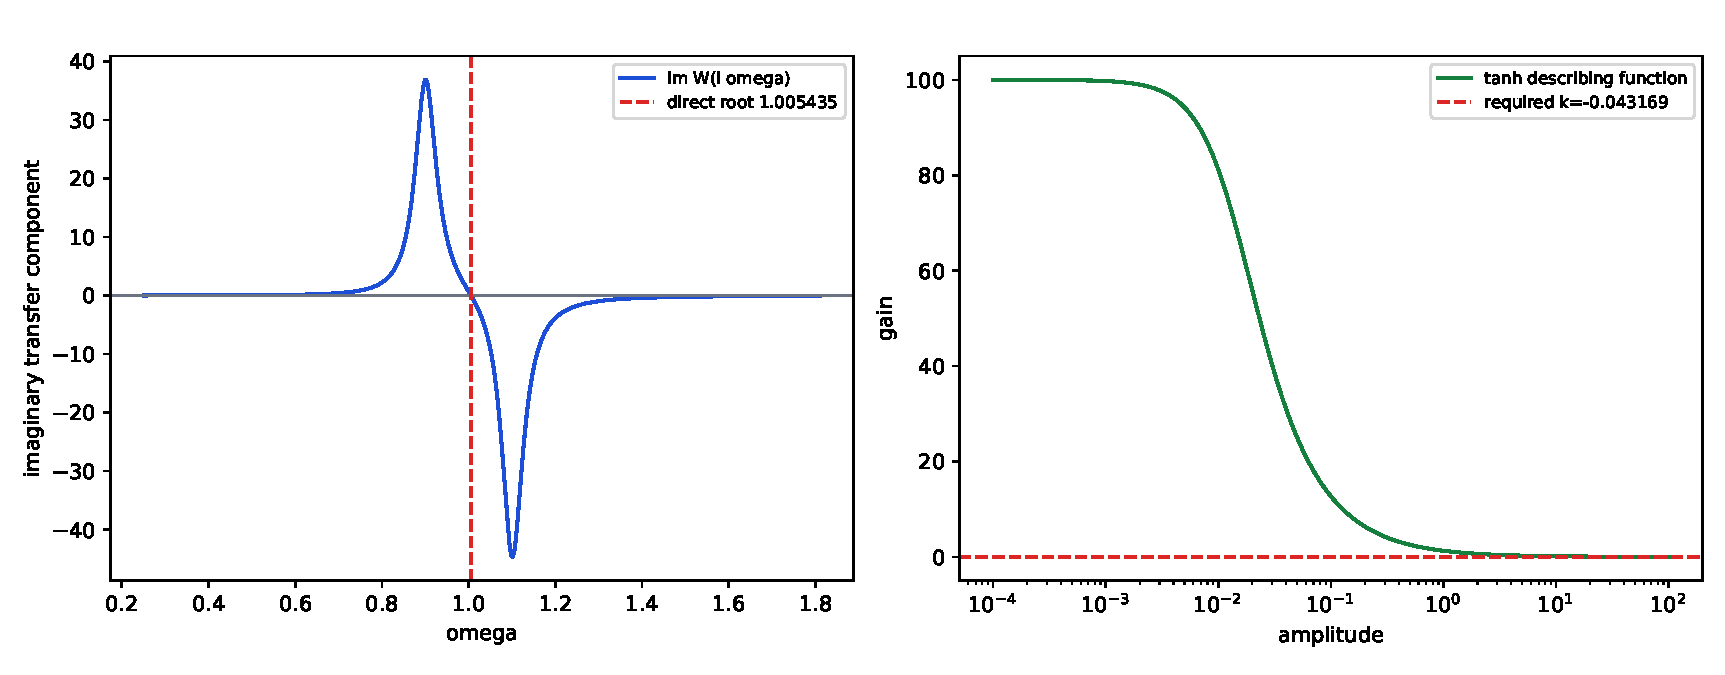
\includegraphics[width=0.94\linewidth,height=0.37\textheight,keepaspectratio]{figures/kalman_fitts/01_direct_route_incompatibility.pdf}\\[-0.25em]
{\footnotesize Kalman--Fitts: incompatibilidad del cierre armónico directo.}
\end{center}
\vfill
\begin{center}
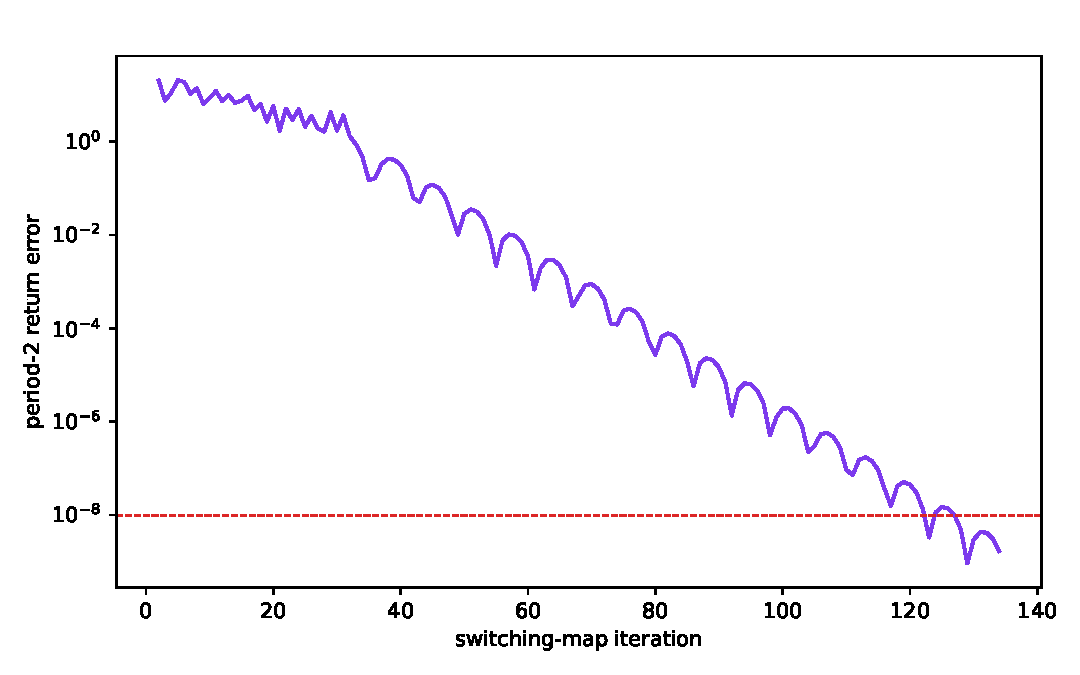
\includegraphics[width=0.94\linewidth,height=0.37\textheight,keepaspectratio]{figures/kalman_fitts/02_switching_map_convergence.pdf}\\[-0.25em]
{\footnotesize Kalman--Fitts: convergencia del mapa de conmutación.}
\end{center}
\clearpage
\begin{center}
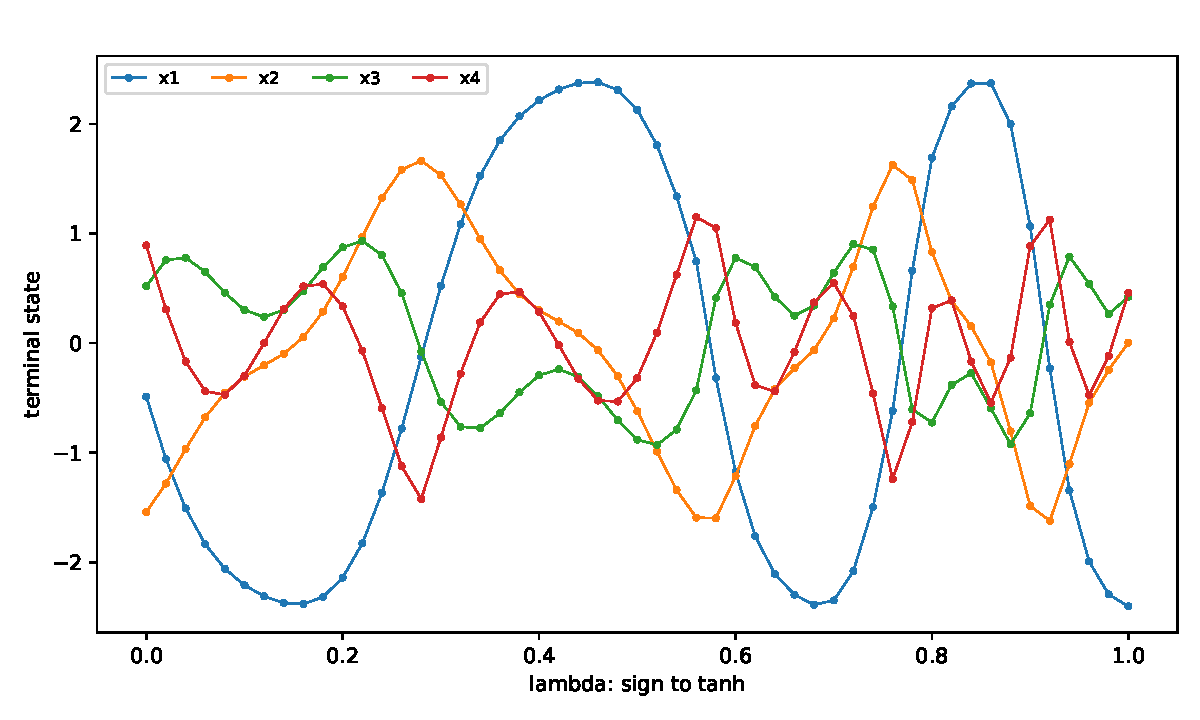
\includegraphics[width=0.94\linewidth,height=0.37\textheight,keepaspectratio]{figures/kalman_fitts/03_sign_to_tanh_continuation.pdf}\\[-0.25em]
{\footnotesize Kalman--Fitts: continuación de la no linealidad signo hacia la tangente hiperbólica.}
\end{center}
\vfill
\begin{center}
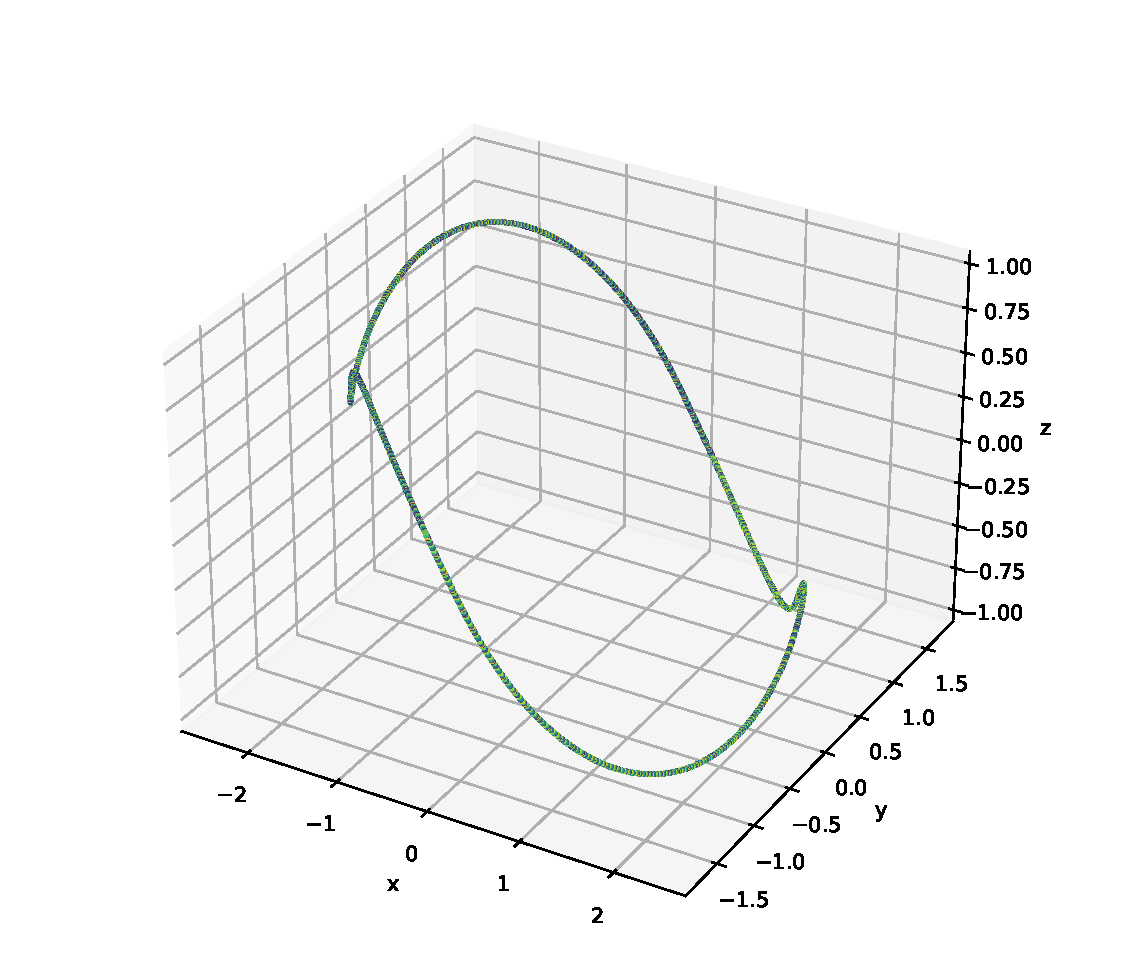
\includegraphics[width=0.94\linewidth,height=0.37\textheight,keepaspectratio]{figures/kalman_fitts/04_hidden_limit_cycle_3d.pdf}\\[-0.25em]
{\footnotesize Kalman--Fitts: trayectoria periódica candidata.}
\end{center}
\clearpage
\begin{center}
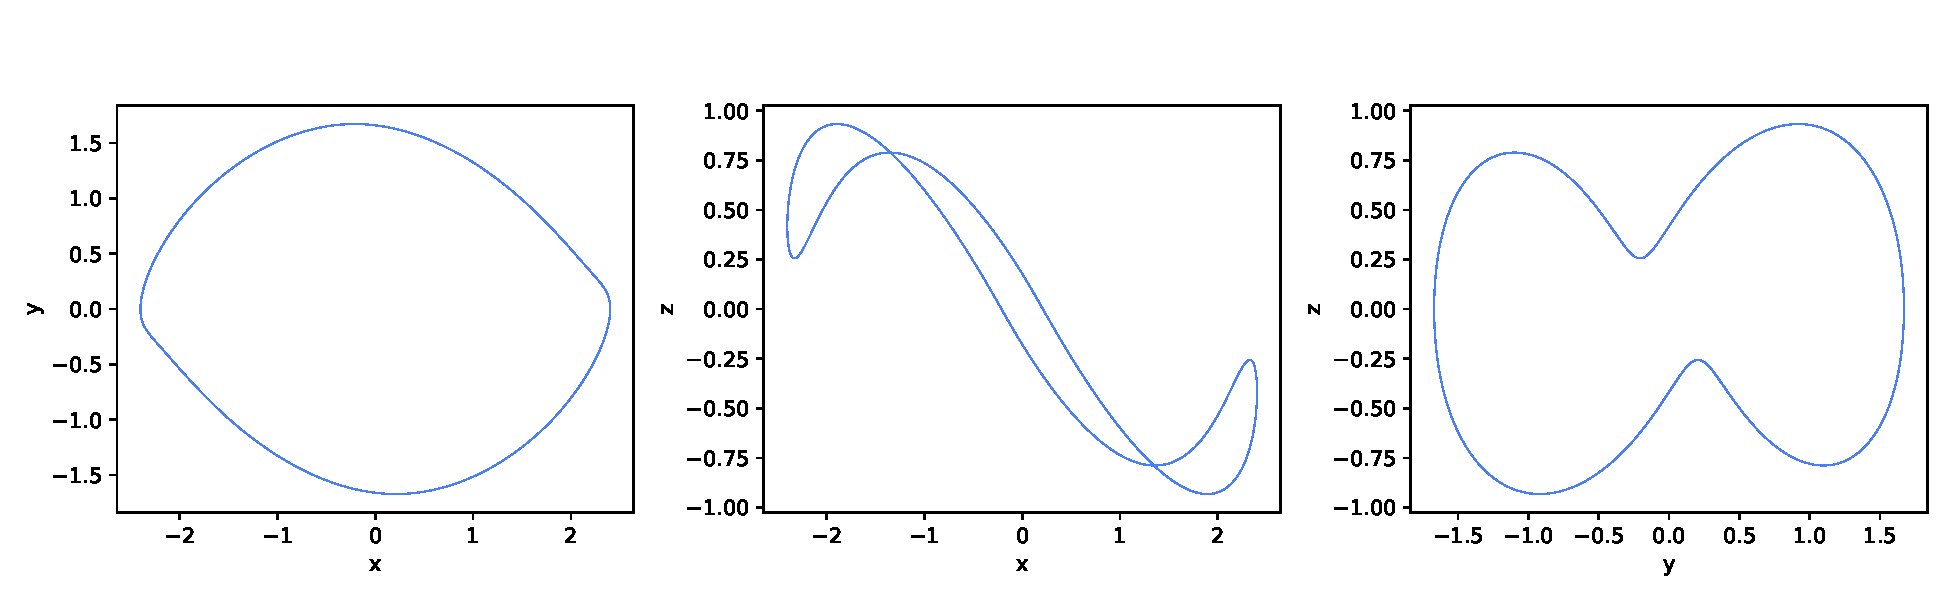
\includegraphics[width=0.94\linewidth,height=0.37\textheight,keepaspectratio]{figures/kalman_fitts/05_hidden_limit_cycle_projections.pdf}\\[-0.25em]
{\footnotesize Kalman--Fitts: proyecciones del ciclo candidato.}
\end{center}
\vfill
\begin{center}
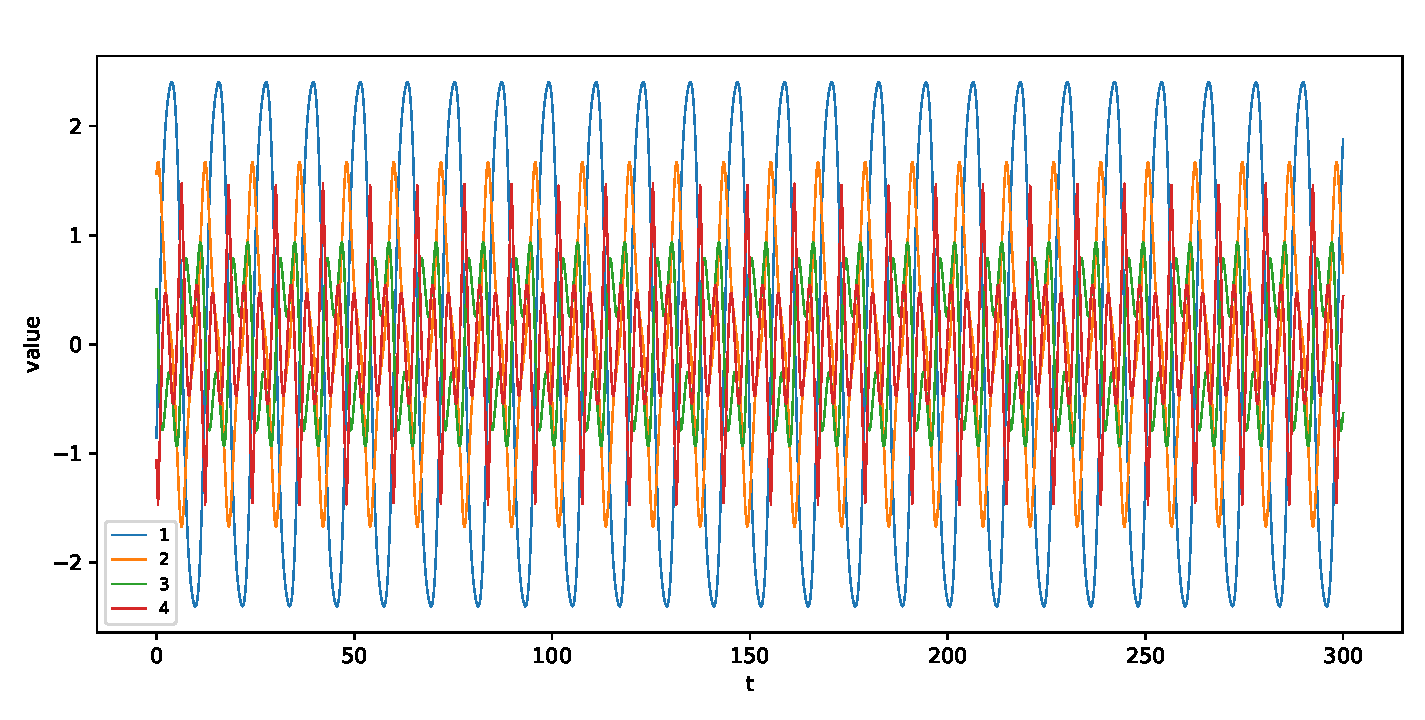
\includegraphics[width=0.94\linewidth,height=0.37\textheight,keepaspectratio]{figures/kalman_fitts/06_hidden_limit_cycle_timeseries.pdf}\\[-0.25em]
{\footnotesize Kalman--Fitts: series temporales del ciclo candidato.}
\end{center}
\clearpage
\begin{center}
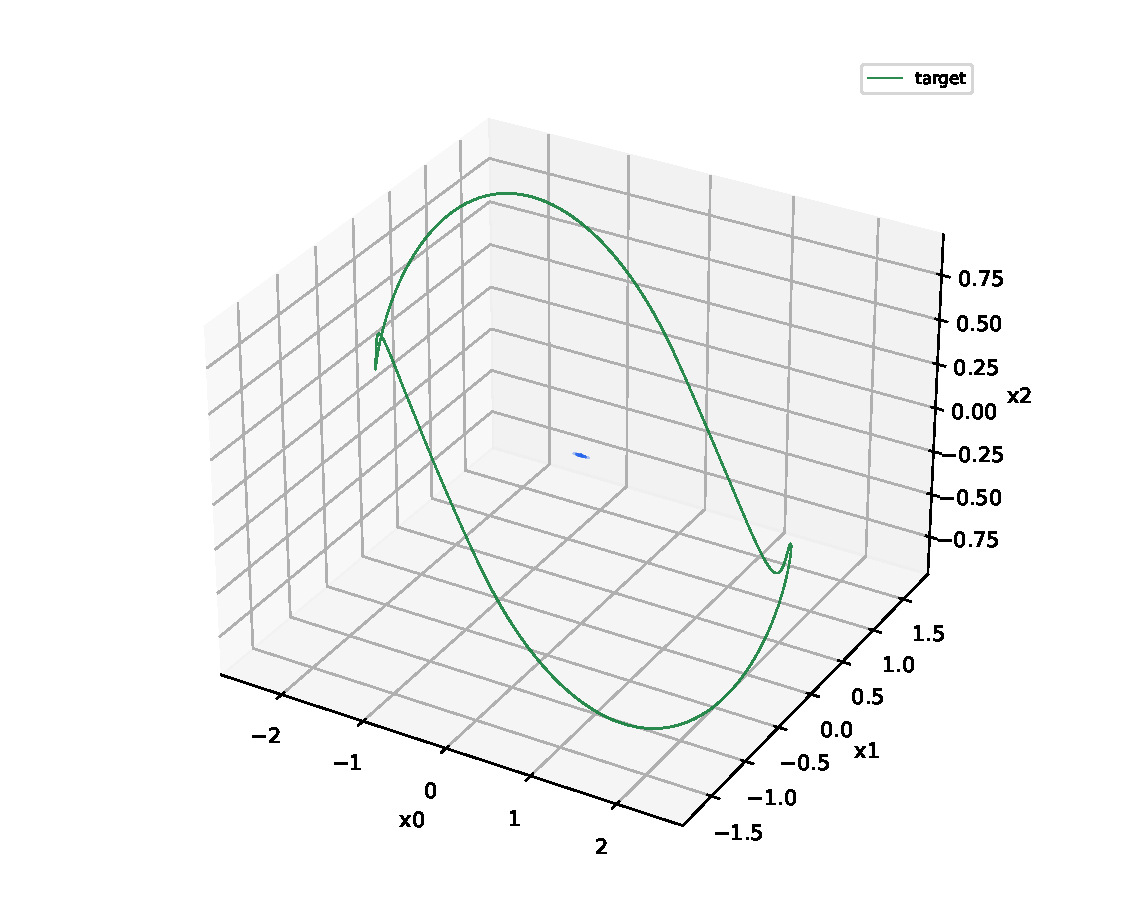
\includegraphics[width=0.94\linewidth,height=0.37\textheight,keepaspectratio]{figures/kalman_fitts/07_equilibrium_neighborhood_controls.pdf}\\[-0.25em]
{\footnotesize Kalman--Fitts: destinos de los sondeos próximos al equilibrio.}
\end{center}
\vfill
\begin{center}
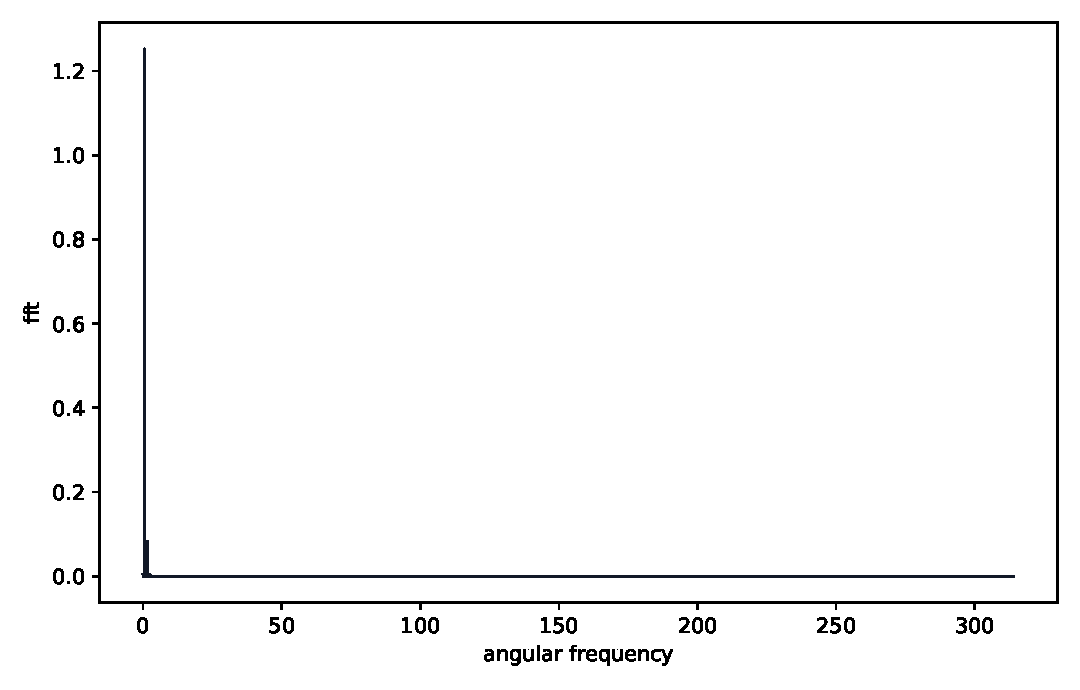
\includegraphics[width=0.94\linewidth,height=0.37\textheight,keepaspectratio]{figures/kalman_fitts/08_kalman_fitts_fft_component_0.pdf}\\[-0.25em]
{\footnotesize Kalman--Fitts: espectro de amplitud de la componente \(x_1\).}
\end{center}
\clearpage
\begin{center}
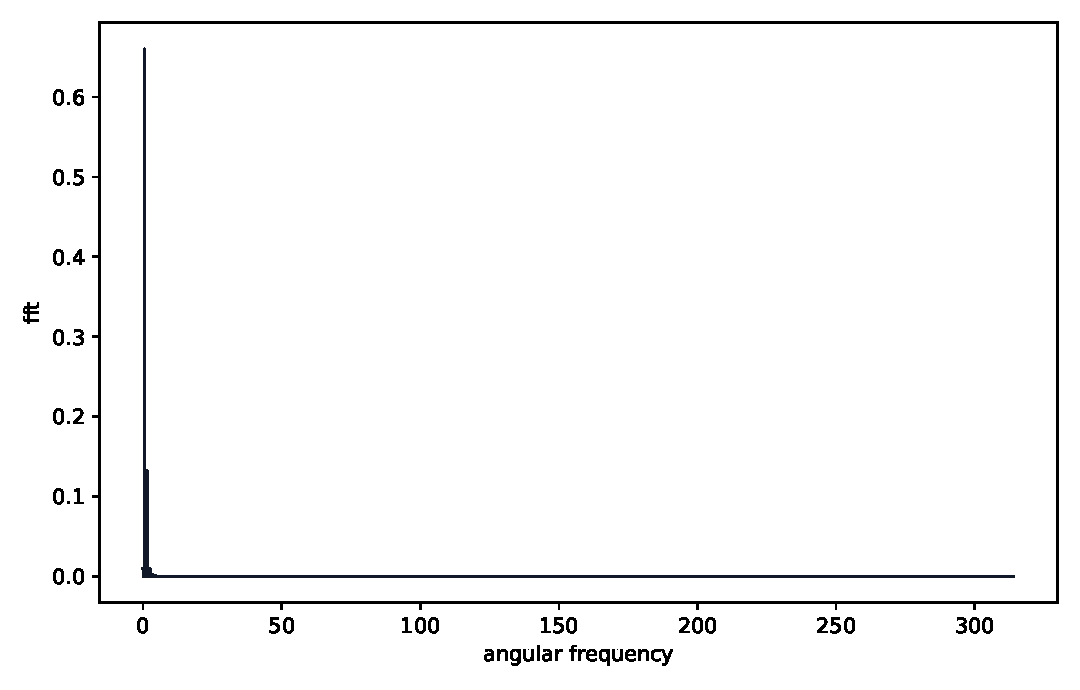
\includegraphics[width=0.94\linewidth,height=0.37\textheight,keepaspectratio]{figures/kalman_fitts/08_kalman_fitts_fft_component_1.pdf}\\[-0.25em]
{\footnotesize Kalman--Fitts: espectro de amplitud de la componente \(x_2\).}
\end{center}
\vfill
\begin{center}
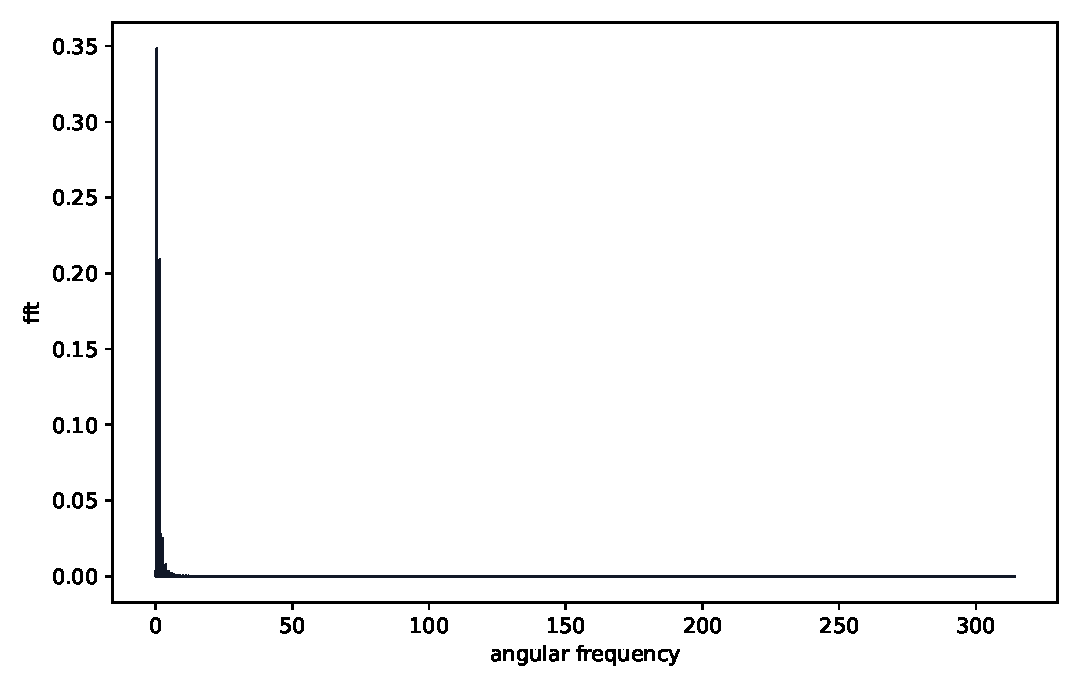
\includegraphics[width=0.94\linewidth,height=0.37\textheight,keepaspectratio]{figures/kalman_fitts/08_kalman_fitts_fft_component_2.pdf}\\[-0.25em]
{\footnotesize Kalman--Fitts: espectro de amplitud de la componente \(x_3\).}
\end{center}
\clearpage
\begin{center}
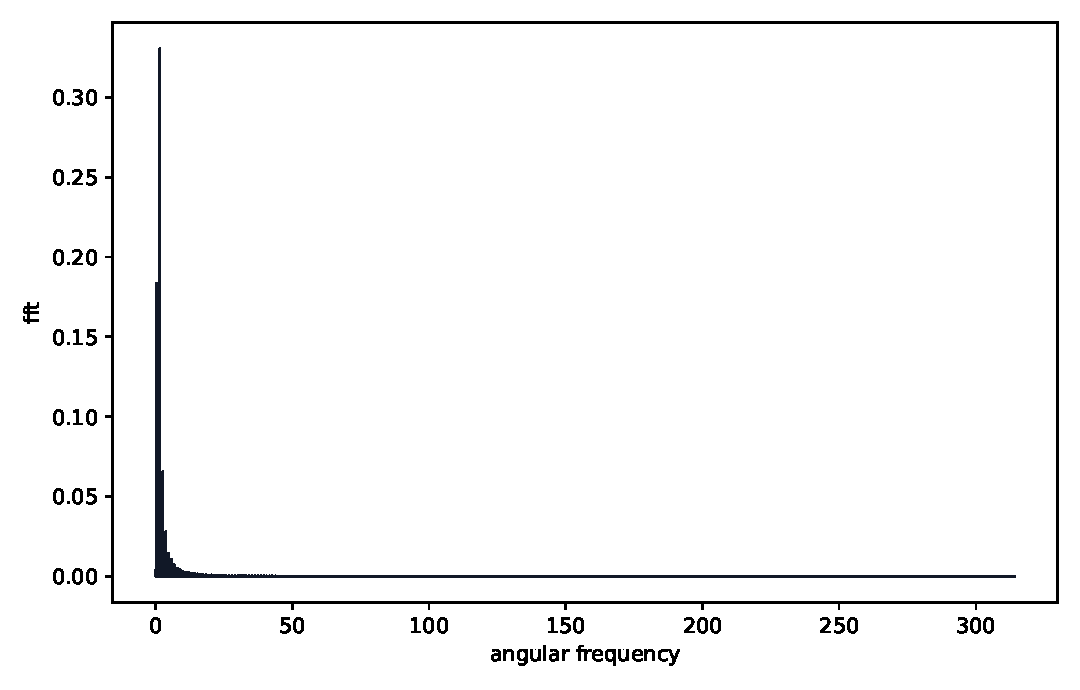
\includegraphics[width=0.94\linewidth,height=0.37\textheight,keepaspectratio]{figures/kalman_fitts/08_kalman_fitts_fft_component_3.pdf}\\[-0.25em]
{\footnotesize Kalman--Fitts: espectro de amplitud de la componente \(x_4\).}
\end{center}
\vfill
\begin{center}
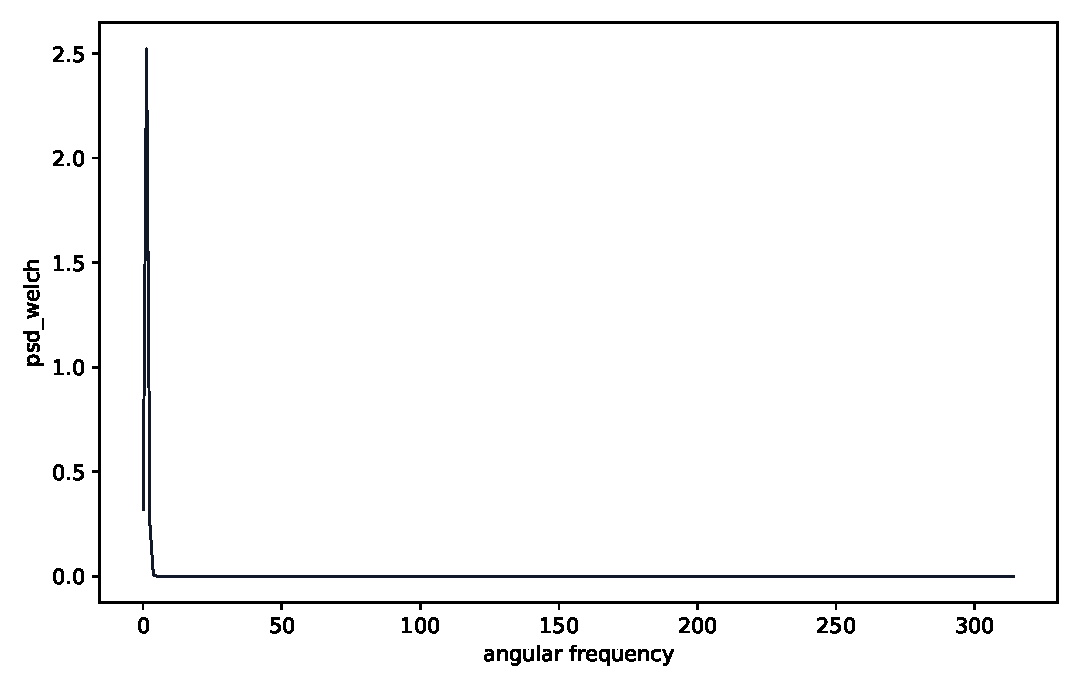
\includegraphics[width=0.94\linewidth,height=0.37\textheight,keepaspectratio]{figures/kalman_fitts/09_kalman_fitts_psd_component_0.pdf}\\[-0.25em]
{\footnotesize Kalman--Fitts: densidad espectral de potencia de la componente \(x_1\).}
\end{center}
\clearpage
\begin{center}
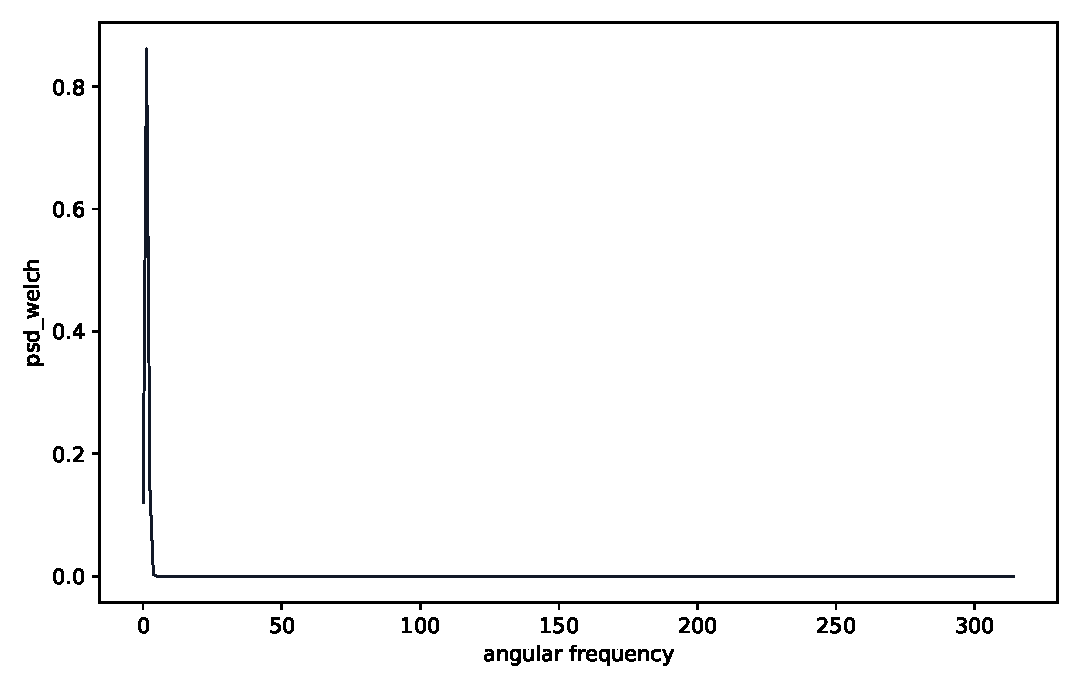
\includegraphics[width=0.94\linewidth,height=0.37\textheight,keepaspectratio]{figures/kalman_fitts/09_kalman_fitts_psd_component_1.pdf}\\[-0.25em]
{\footnotesize Kalman--Fitts: densidad espectral de potencia de la componente \(x_2\).}
\end{center}
\vfill
\begin{center}
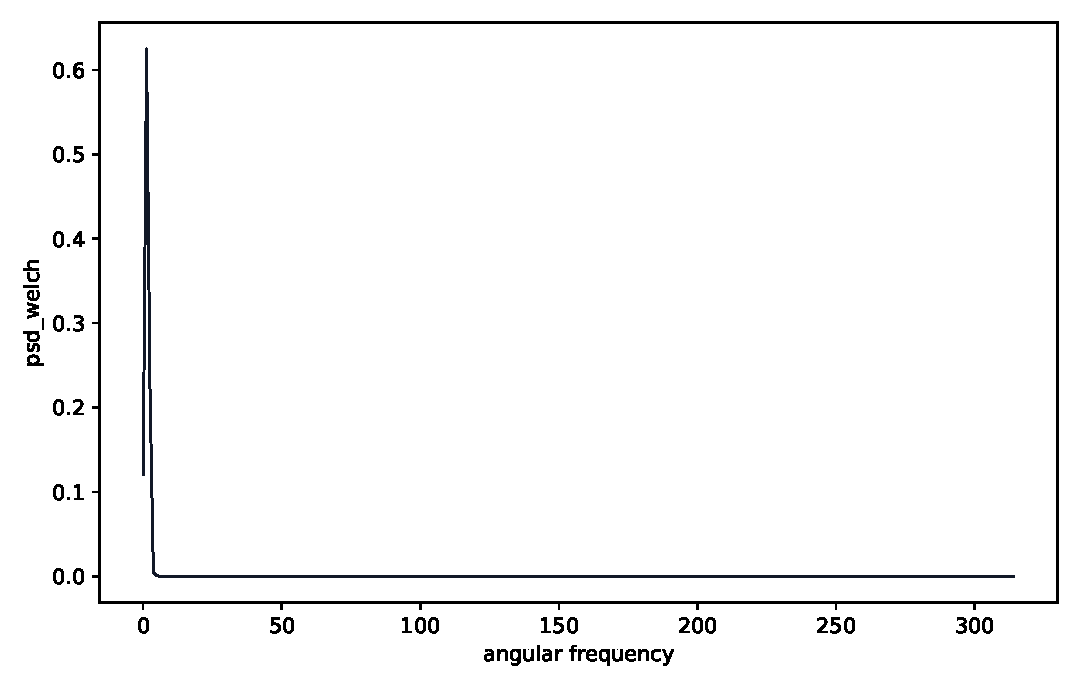
\includegraphics[width=0.94\linewidth,height=0.37\textheight,keepaspectratio]{figures/kalman_fitts/09_kalman_fitts_psd_component_2.pdf}\\[-0.25em]
{\footnotesize Kalman--Fitts: densidad espectral de potencia de la componente \(x_3\).}
\end{center}
\clearpage
\begin{center}
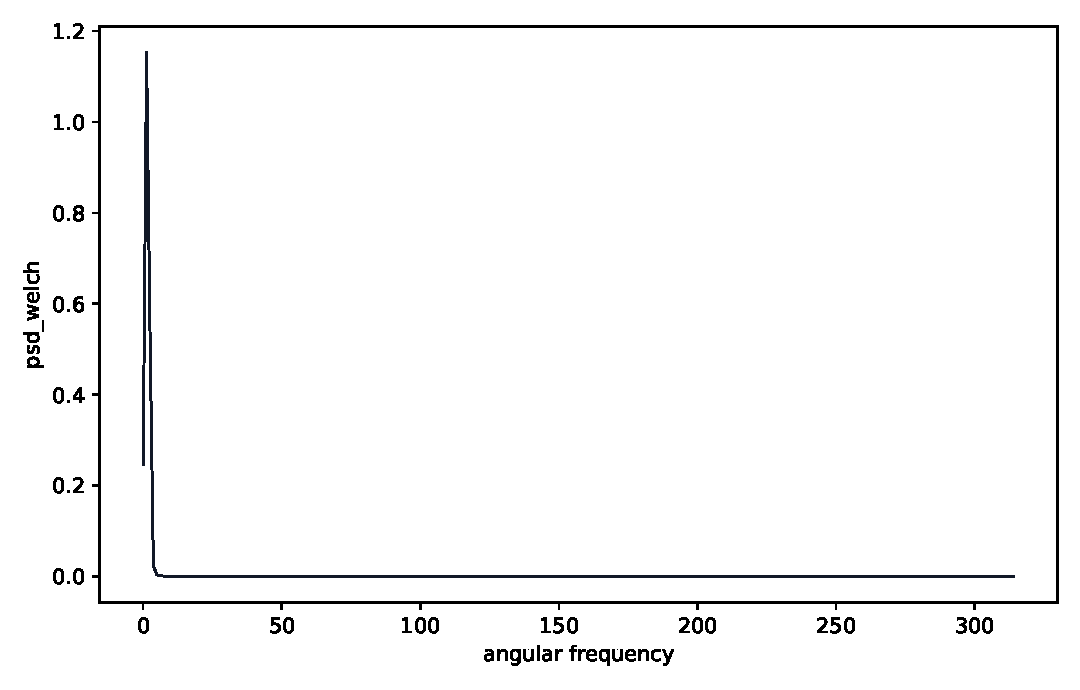
\includegraphics[width=0.94\linewidth,height=0.37\textheight,keepaspectratio]{figures/kalman_fitts/09_kalman_fitts_psd_component_3.pdf}\\[-0.25em]
{\footnotesize Kalman--Fitts: densidad espectral de potencia de la componente \(x_4\).}
\end{center}
\vfill
\begin{center}
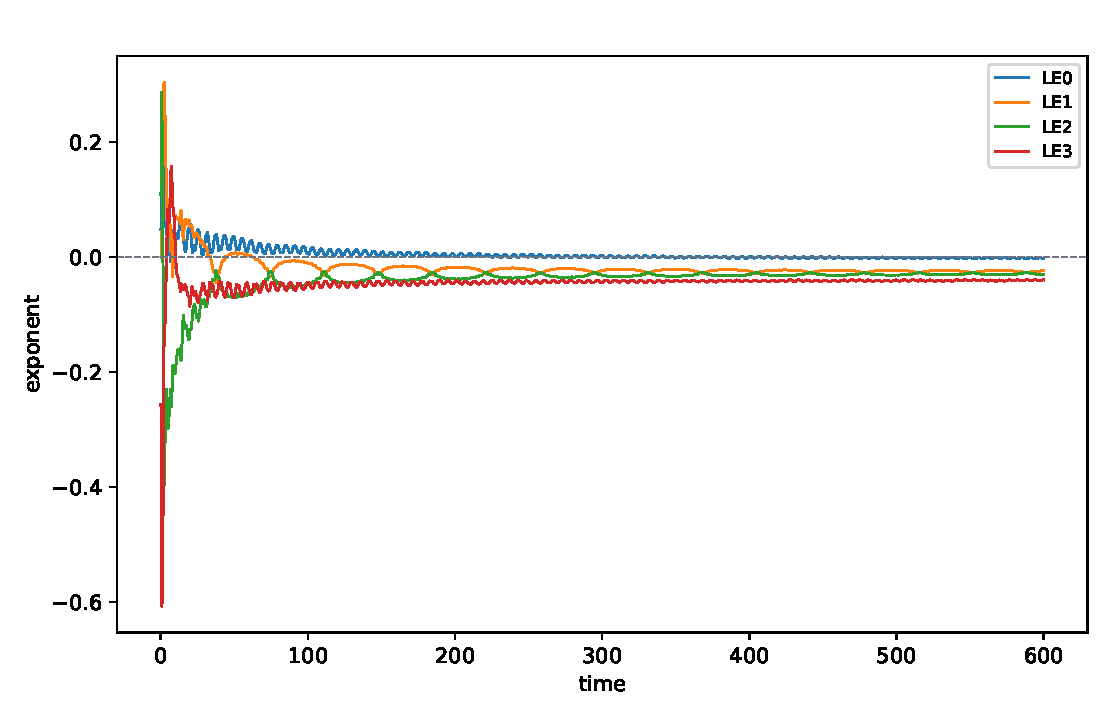
\includegraphics[width=0.94\linewidth,height=0.37\textheight,keepaspectratio]{figures/kalman_fitts/10_lyapunov_convergence.pdf}\\[-0.25em]
{\footnotesize Kalman--Fitts: evolución de las estimaciones de Lyapunov.}
\end{center}
\clearpage
\clearpage
\subsection{MAVPD entero: verificación de periodicidad y control negativo}
Ramas D0, continuación, candidato externo, series, amplitud espectral y comparación del control negativo.

\begin{center}
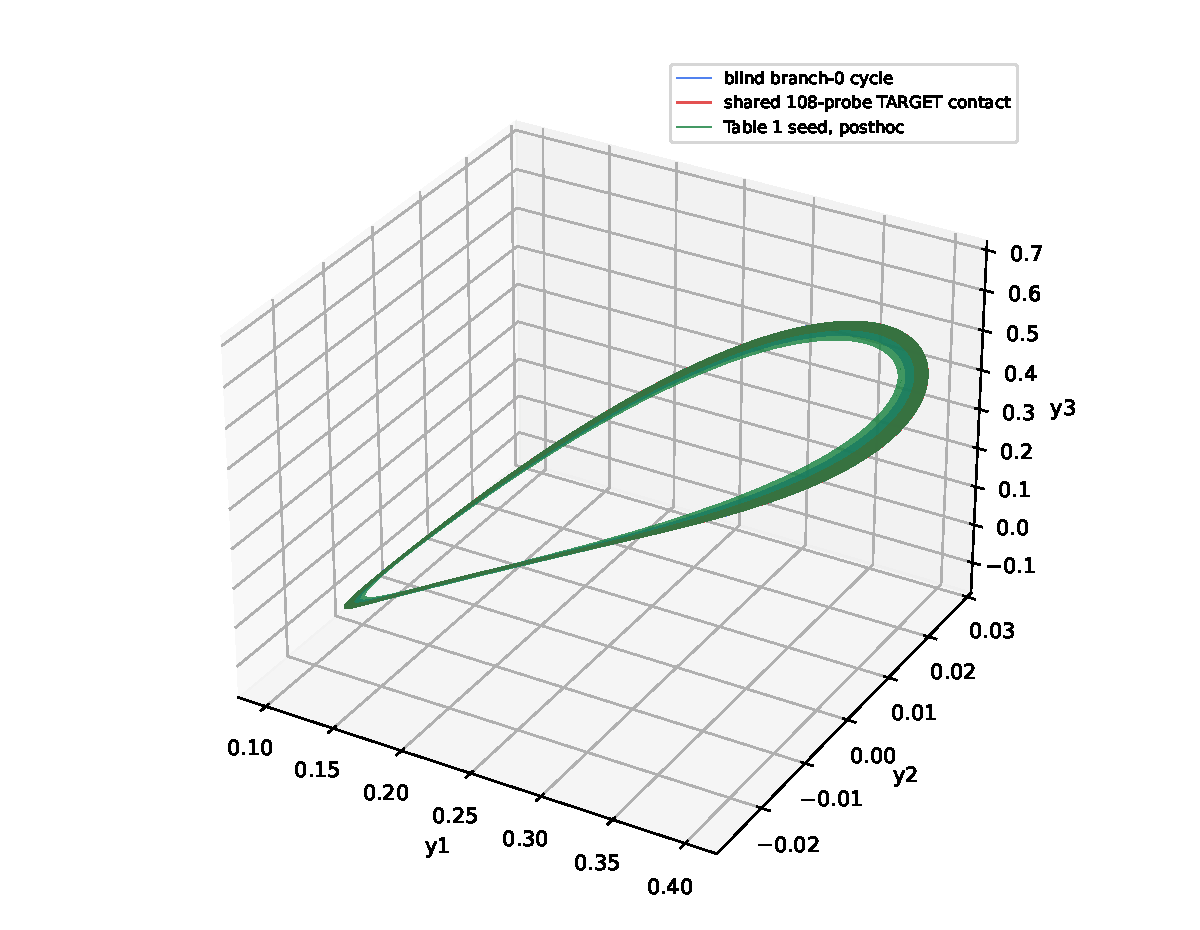
\includegraphics[width=0.94\linewidth,height=0.37\textheight,keepaspectratio]{figures/mavpd_audit/negative_xi3p5_comparison.pdf}\\[-0.25em]
{\footnotesize MAVPD: comparación con el control de contacto, \(\xi=3.5\).}
\end{center}
\vfill
\begin{center}
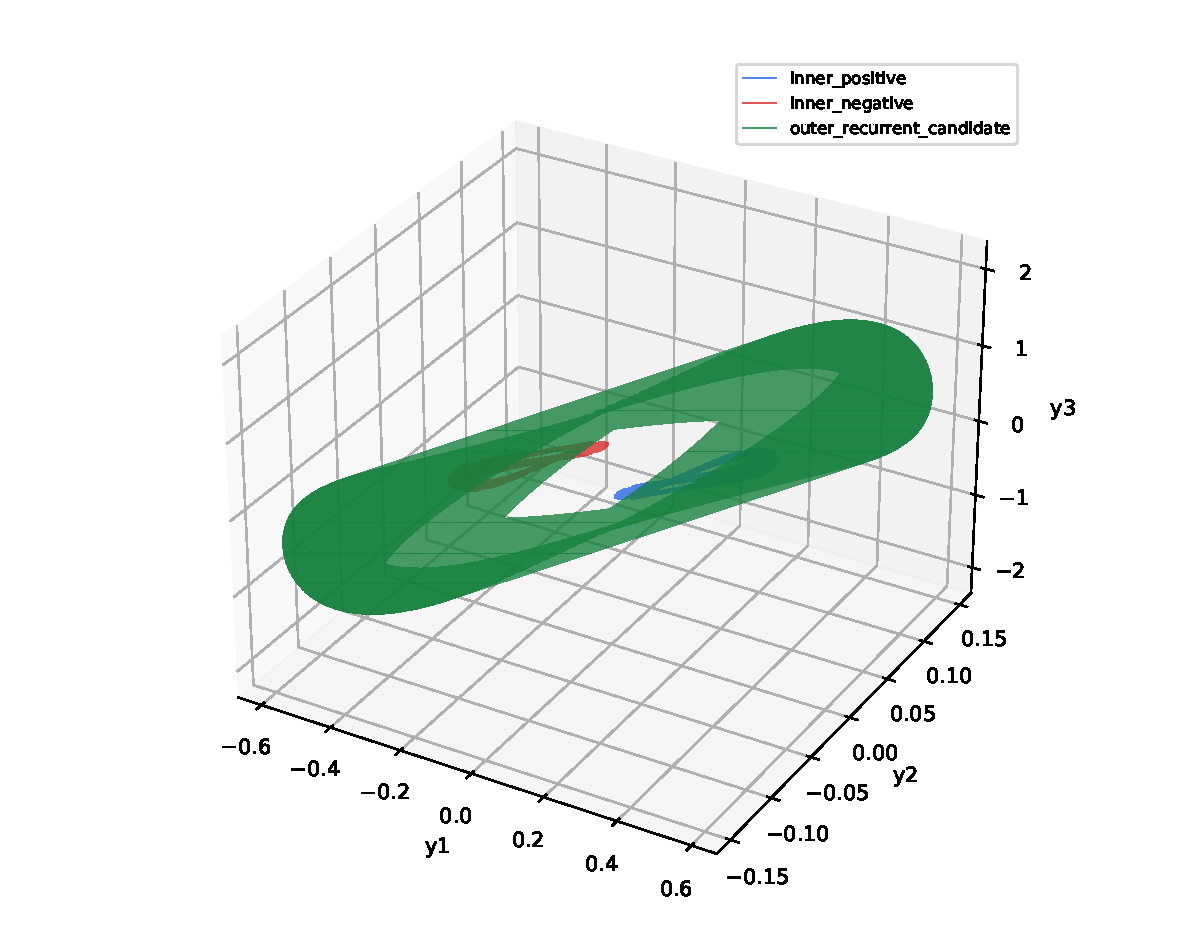
\includegraphics[width=0.94\linewidth,height=0.37\textheight,keepaspectratio]{figures/mavpd_audit/primary_blind_clusters.pdf}\\[-0.25em]
{\footnotesize MAVPD: agrupación de destinos de la búsqueda de condiciones iniciales.}
\end{center}
\clearpage
\begin{center}
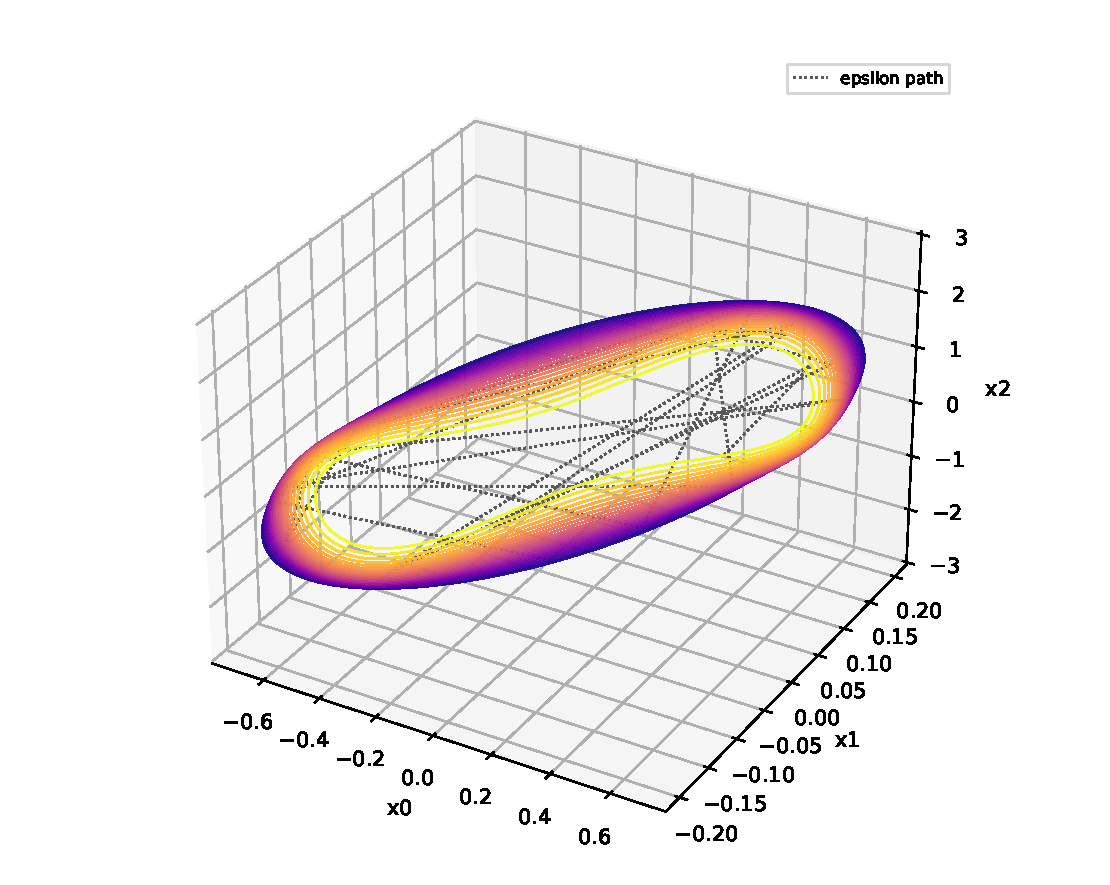
\includegraphics[width=0.94\linewidth,height=0.37\textheight,keepaspectratio]{figures/mavpd_audit/primary_lambda_continuation.pdf}\\[-0.25em]
{\footnotesize MAVPD: continuación del parámetro auxiliar.}
\end{center}
\vfill
\begin{center}
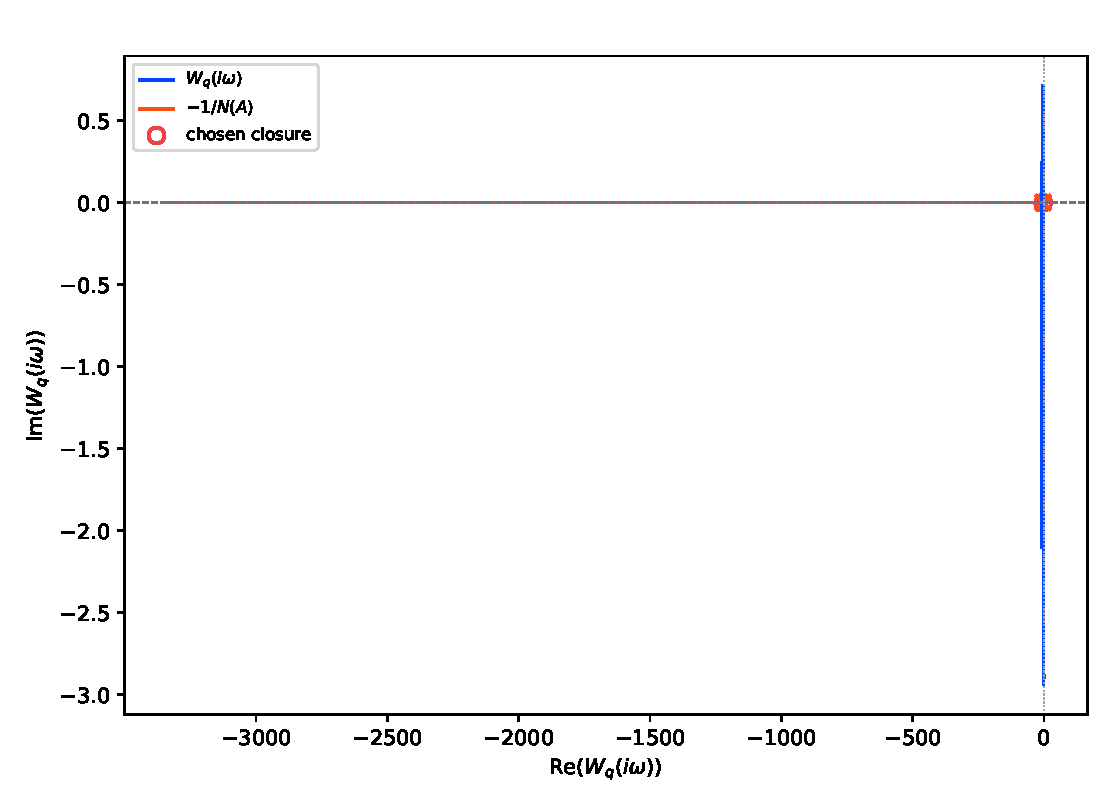
\includegraphics[width=0.94\linewidth,height=0.37\textheight,keepaspectratio]{figures/mavpd_audit/primary_nyquist_df.pdf}\\[-0.25em]
{\footnotesize MAVPD: diagrama de Nyquist y cierre de función descriptiva.}
\end{center}
\clearpage
\begin{center}
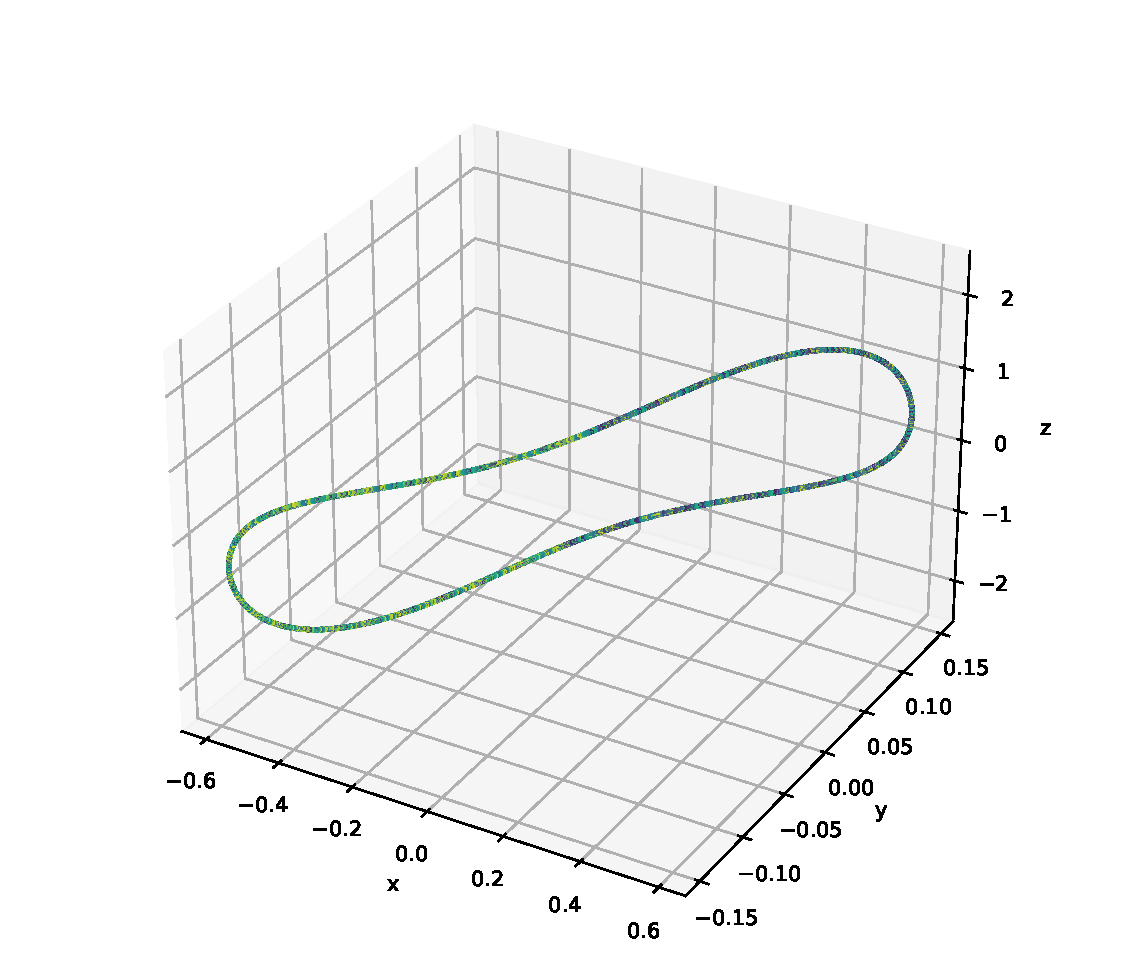
\includegraphics[width=0.94\linewidth,height=0.37\textheight,keepaspectratio]{figures/mavpd_audit/primary_outer_candidate.pdf}\\[-0.25em]
{\footnotesize MAVPD: trayectoria periódica externa candidata.}
\end{center}
\vfill
\begin{center}
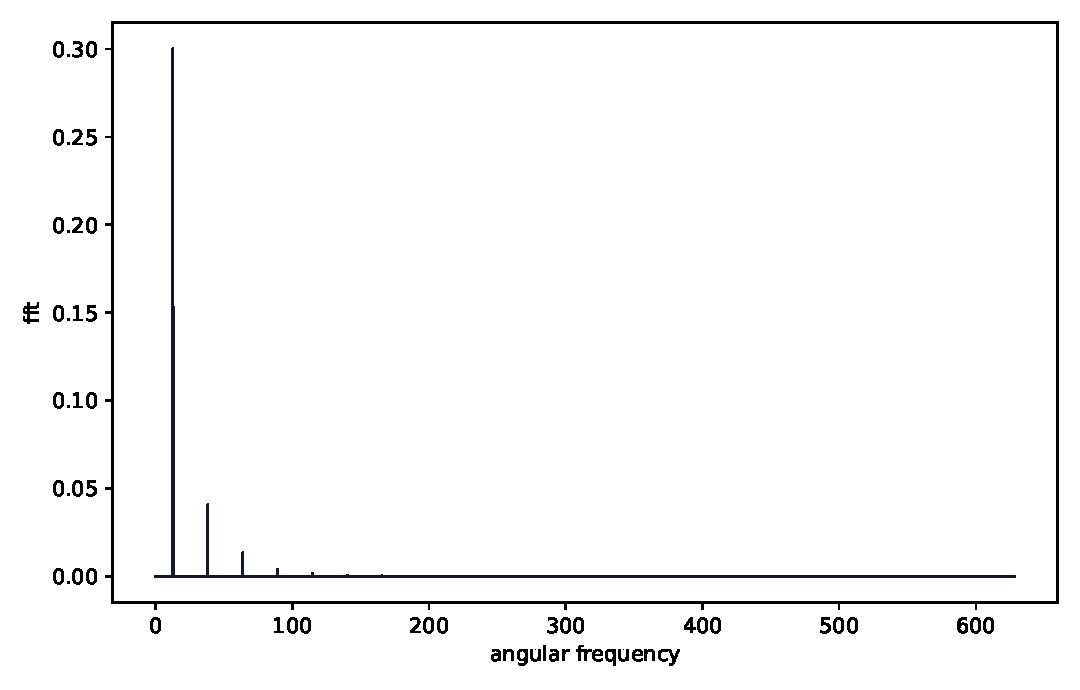
\includegraphics[width=0.94\linewidth,height=0.37\textheight,keepaspectratio]{figures/mavpd_audit/primary_outer_fft_component_0.pdf}\\[-0.25em]
{\footnotesize MAVPD: espectro de amplitud de la componente \(x_1\).}
\end{center}
\clearpage
\begin{center}
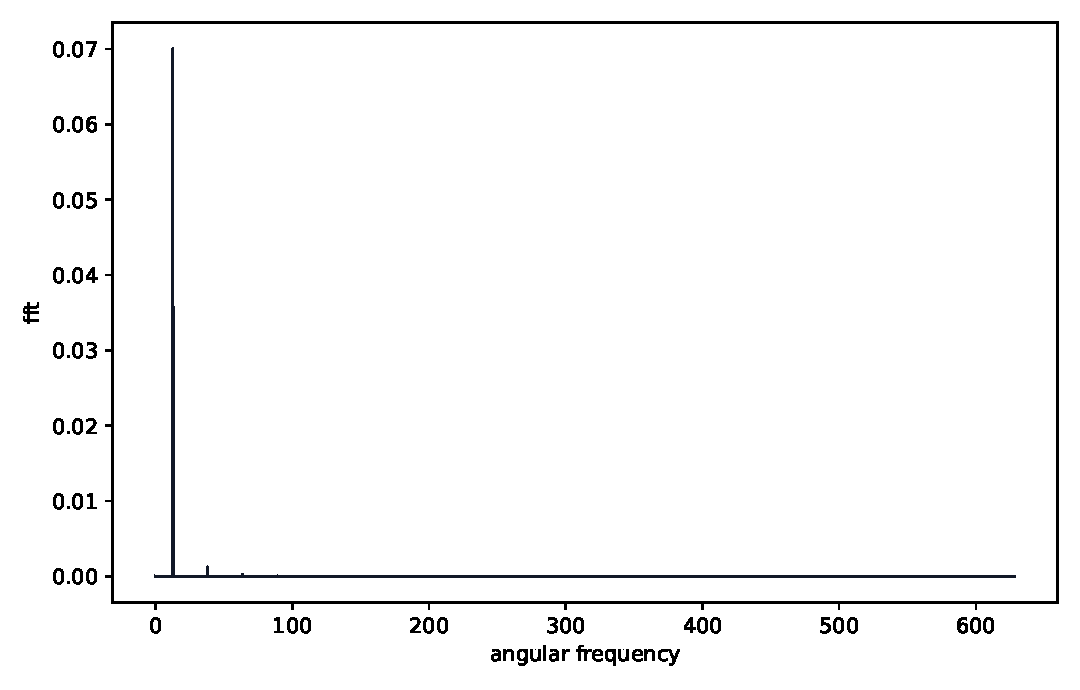
\includegraphics[width=0.94\linewidth,height=0.37\textheight,keepaspectratio]{figures/mavpd_audit/primary_outer_fft_component_1.pdf}\\[-0.25em]
{\footnotesize MAVPD: espectro de amplitud de la componente \(x_2\).}
\end{center}
\vfill
\begin{center}
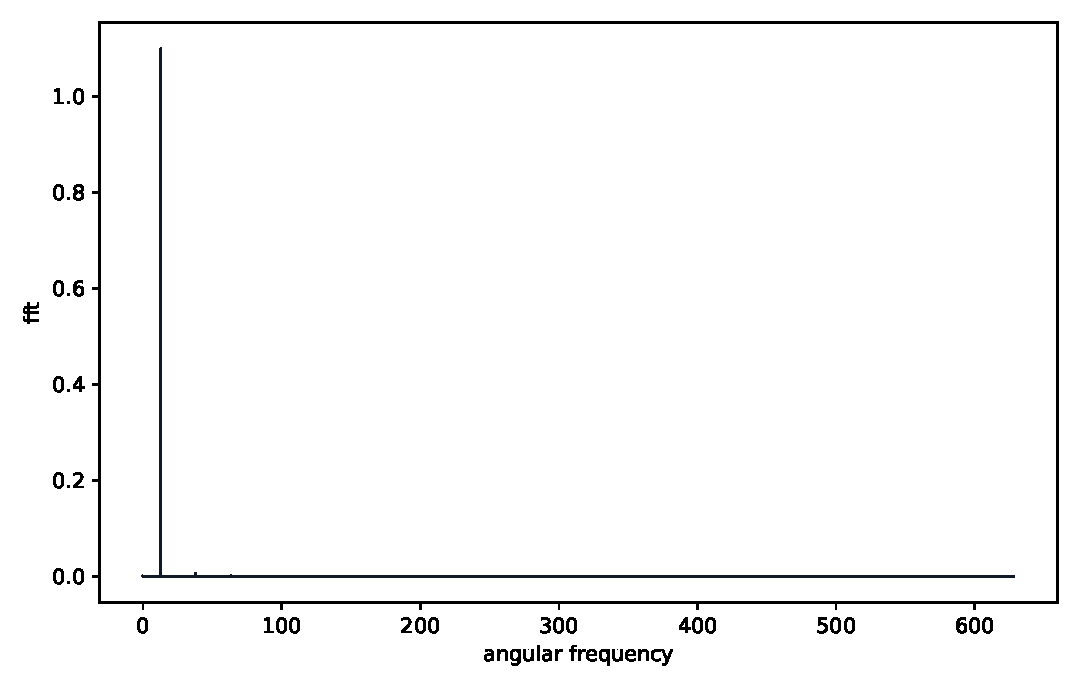
\includegraphics[width=0.94\linewidth,height=0.37\textheight,keepaspectratio]{figures/mavpd_audit/primary_outer_fft_component_2.pdf}\\[-0.25em]
{\footnotesize MAVPD: espectro de amplitud de la componente \(x_3\).}
\end{center}
\clearpage
\begin{center}
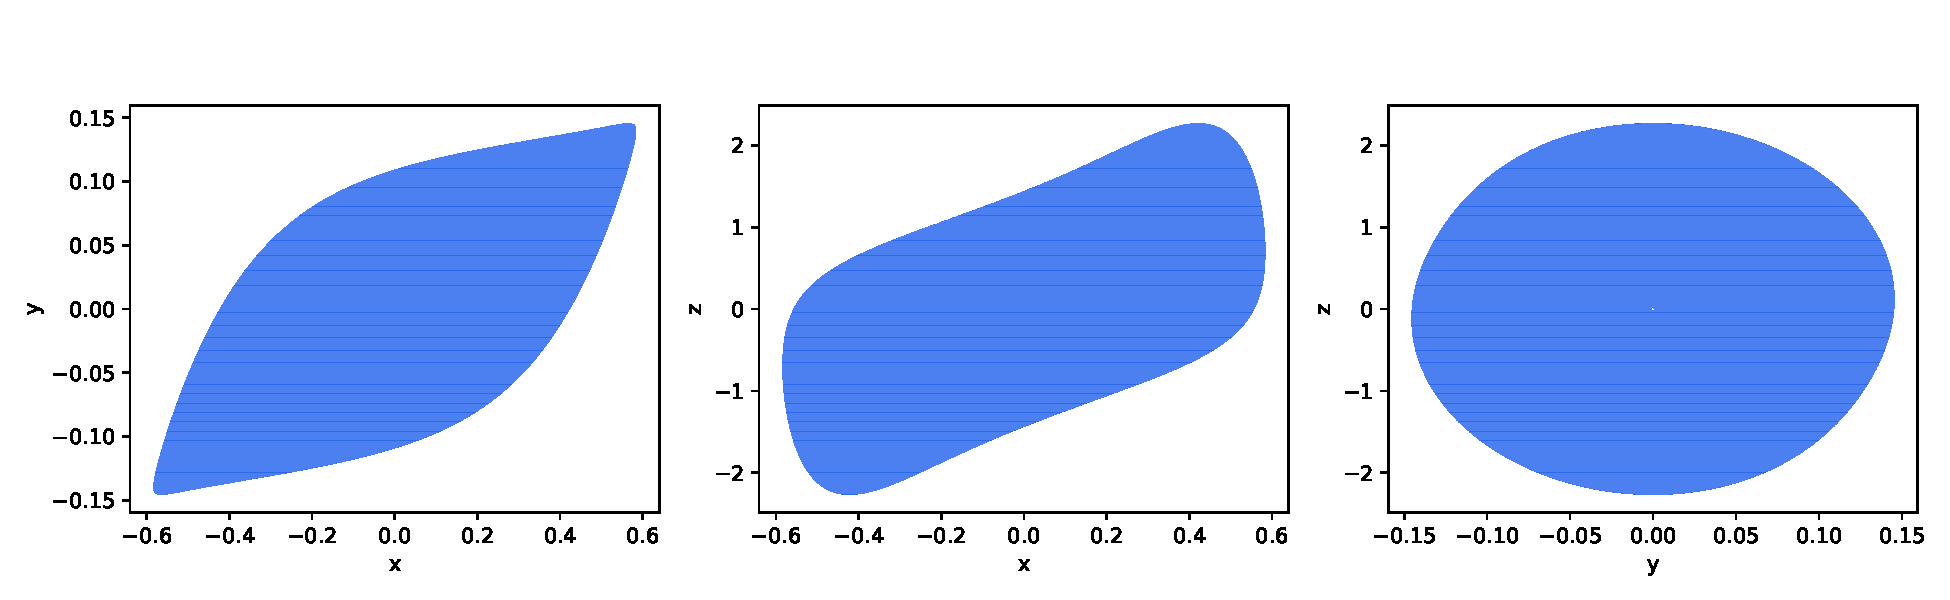
\includegraphics[width=0.94\linewidth,height=0.37\textheight,keepaspectratio]{figures/mavpd_audit/primary_outer_projections.pdf}\\[-0.25em]
{\footnotesize MAVPD: proyecciones de la trayectoria externa.}
\end{center}
\vfill
\begin{center}
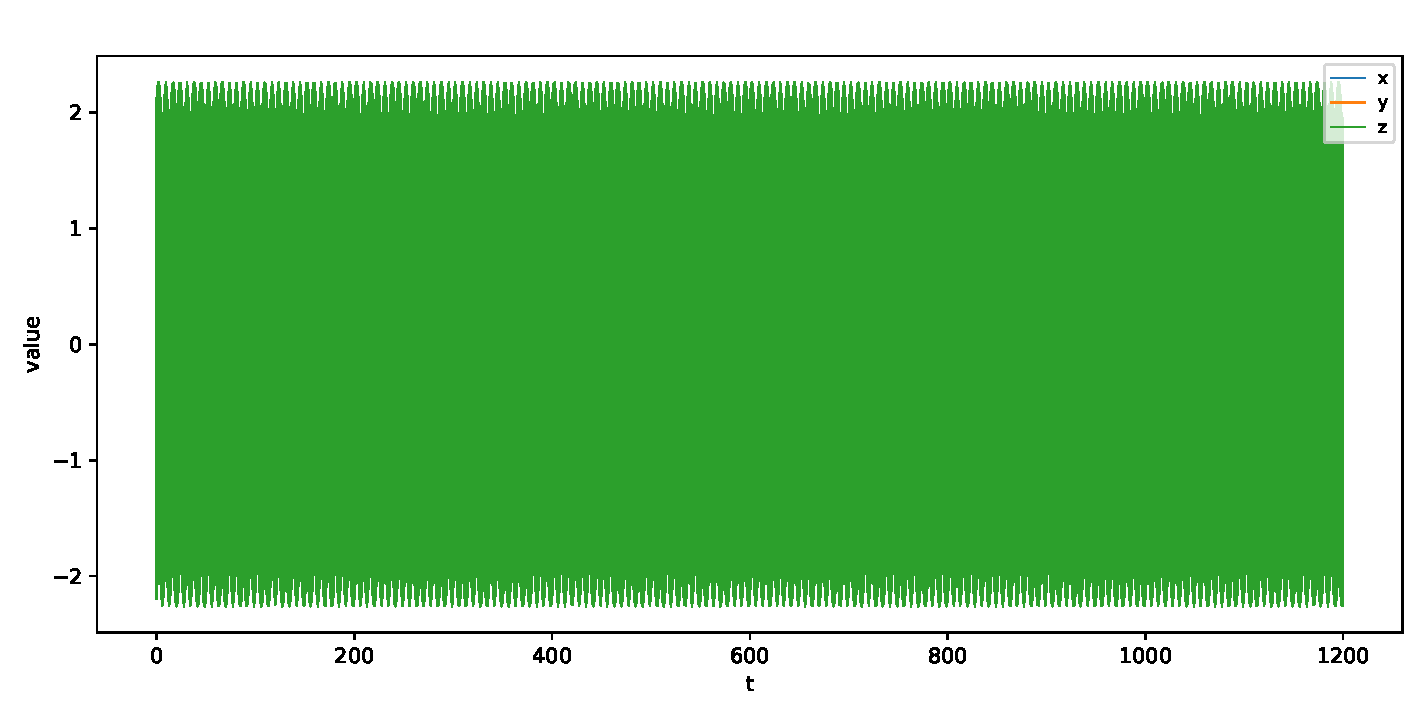
\includegraphics[width=0.94\linewidth,height=0.37\textheight,keepaspectratio]{figures/mavpd_audit/primary_outer_timeseries.pdf}\\[-0.25em]
{\footnotesize MAVPD: series temporales de la trayectoria externa.}
\end{center}
\clearpage
\begin{center}
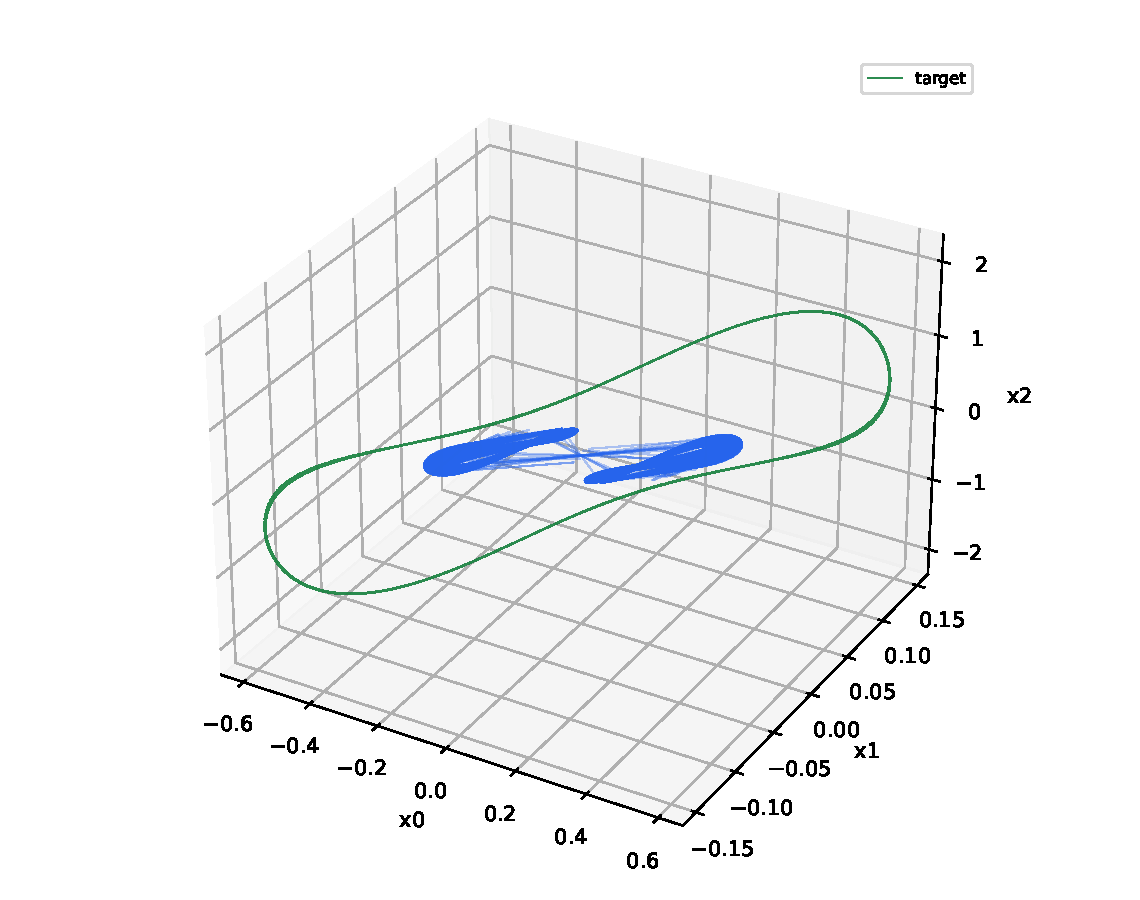
\includegraphics[width=0.94\linewidth,height=0.37\textheight,keepaspectratio]{figures/mavpd_audit/primary_shared_hiddenness_controls.pdf}\\[-0.25em]
{\footnotesize MAVPD: sondeos de cuenca próximos a los equilibrios.}
\end{center}
\vfill
\begin{center}
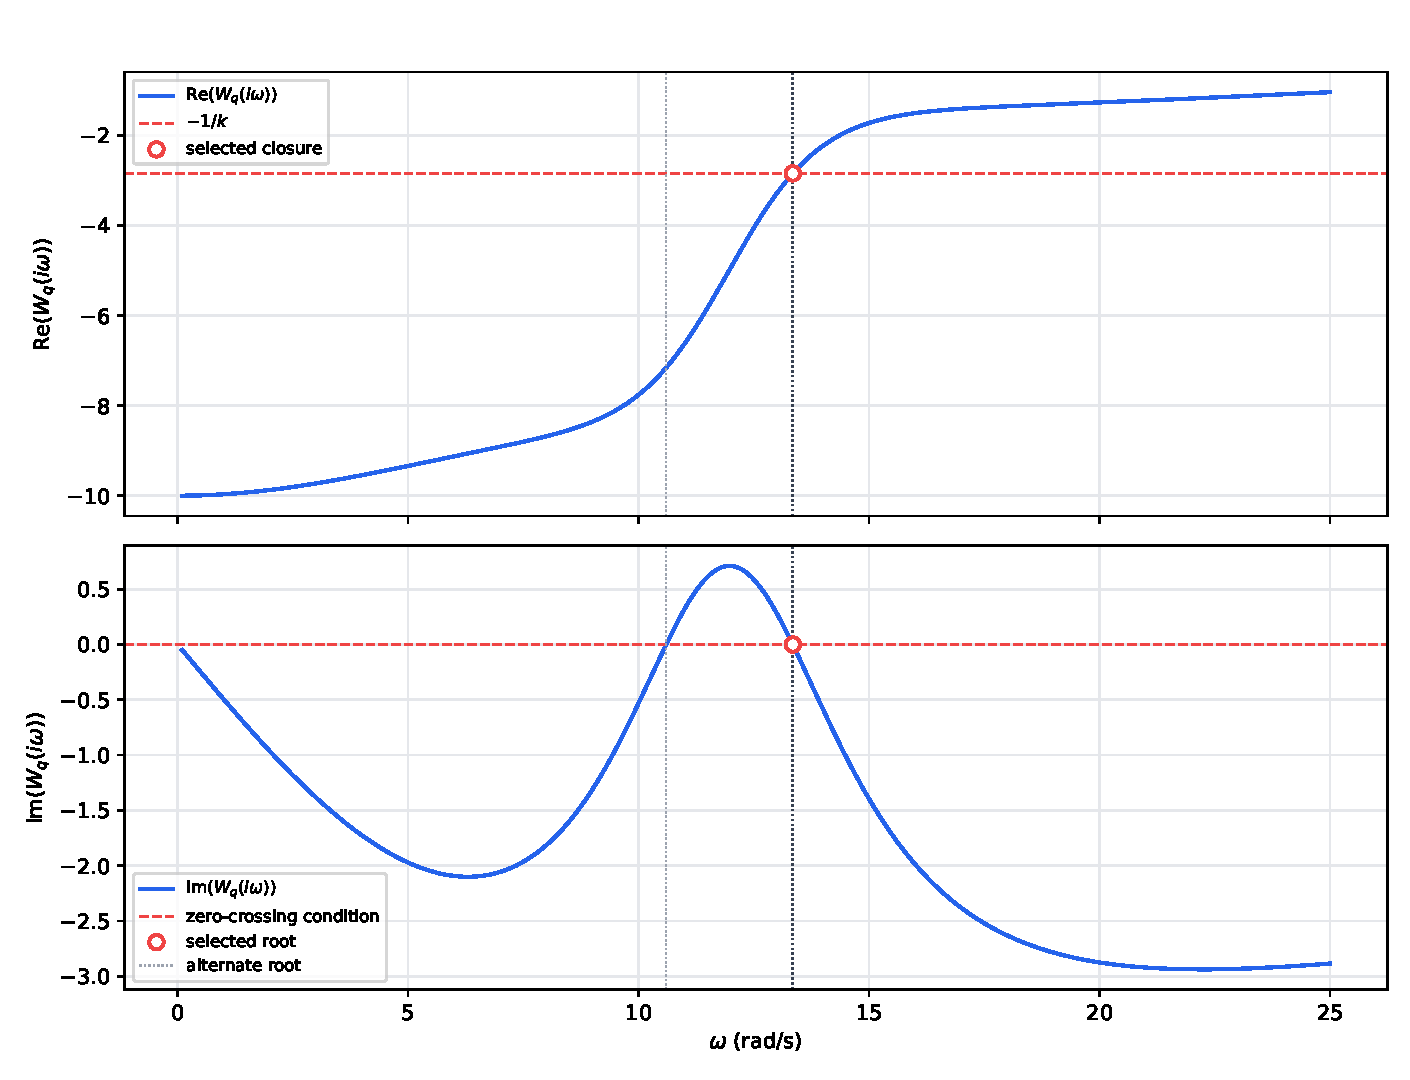
\includegraphics[width=0.94\linewidth,height=0.37\textheight,keepaspectratio]{figures/mavpd_audit/primary_transfer_components.pdf}\\[-0.25em]
{\footnotesize MAVPD: partes real e imaginaria de la transferencia.}
\end{center}
\clearpage
\clearpage
\subsection{MAVPD entero: candidato caótico local}
Cribado de continuación, retratos, series, Lyapunov, espectro normalizado, Poincaré y sondeos locales.

\begin{center}
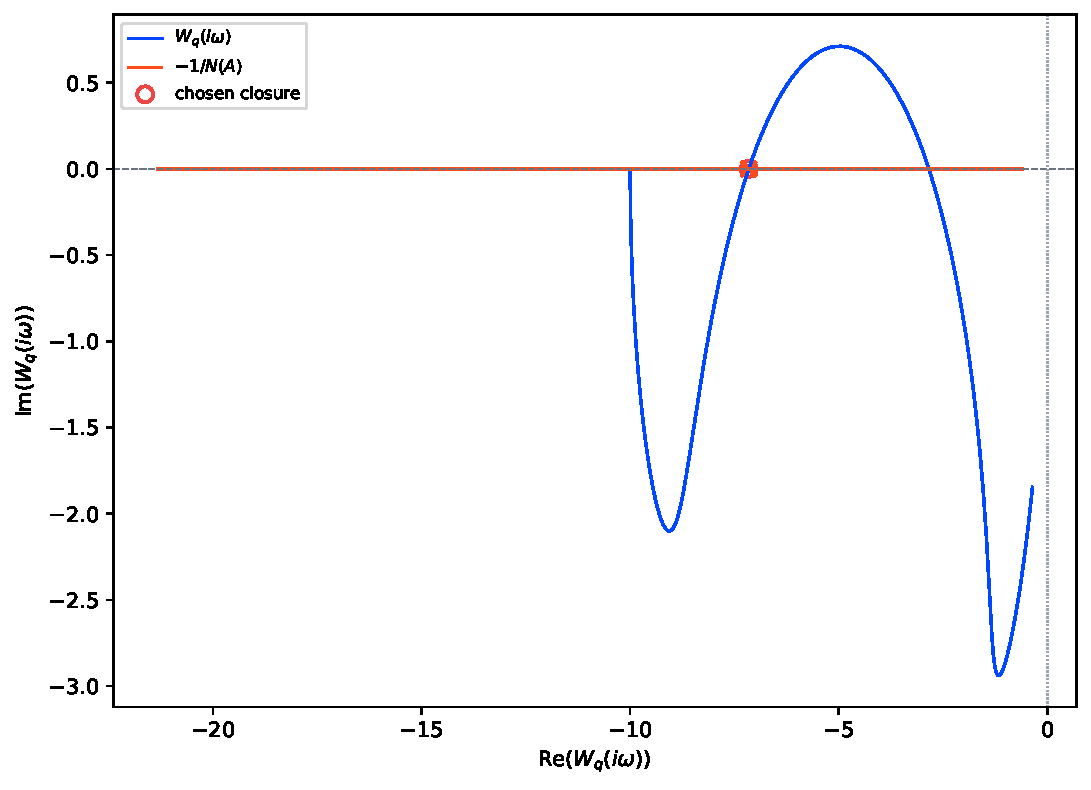
\includegraphics[width=0.94\linewidth,height=0.37\textheight,keepaspectratio]{figures/mavpd_chaos/00_nyquist_direct_seed.pdf}\\[-0.25em]
{\footnotesize MAVPD: Nyquist y construcción de la semilla del candidato caótico.}
\end{center}
\vfill
\begin{center}
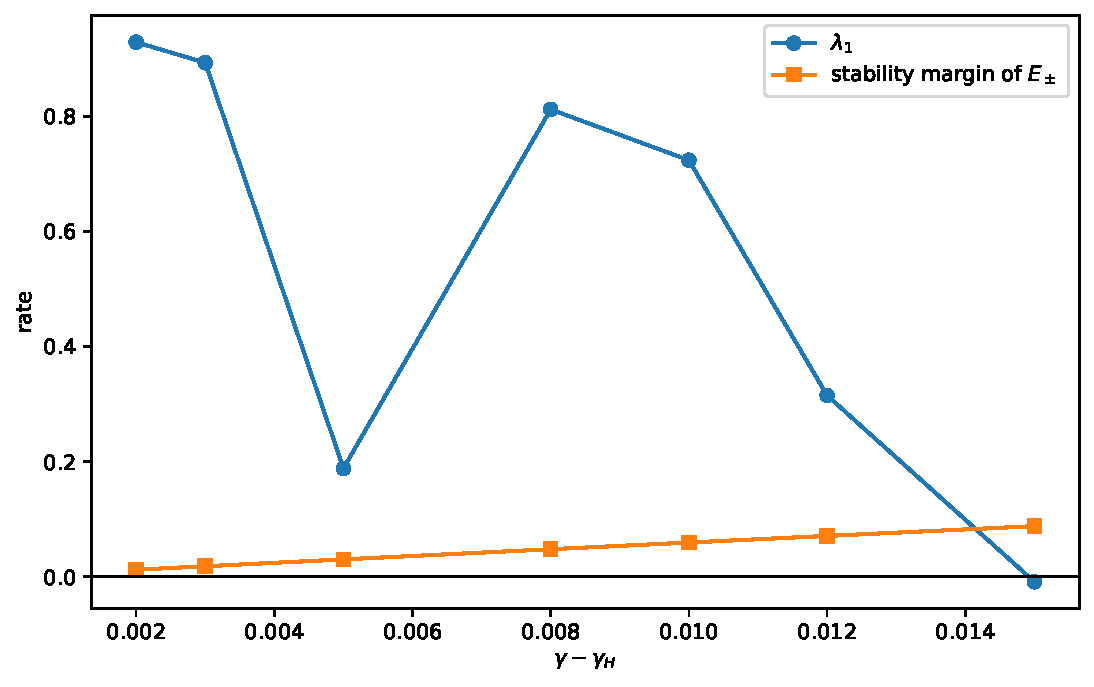
\includegraphics[width=0.94\linewidth,height=0.37\textheight,keepaspectratio]{figures/mavpd_chaos/03_continuation_screen.pdf}\\[-0.25em]
{\footnotesize MAVPD: respuesta durante la continuación del candidato caótico.}
\end{center}
\clearpage
\begin{center}
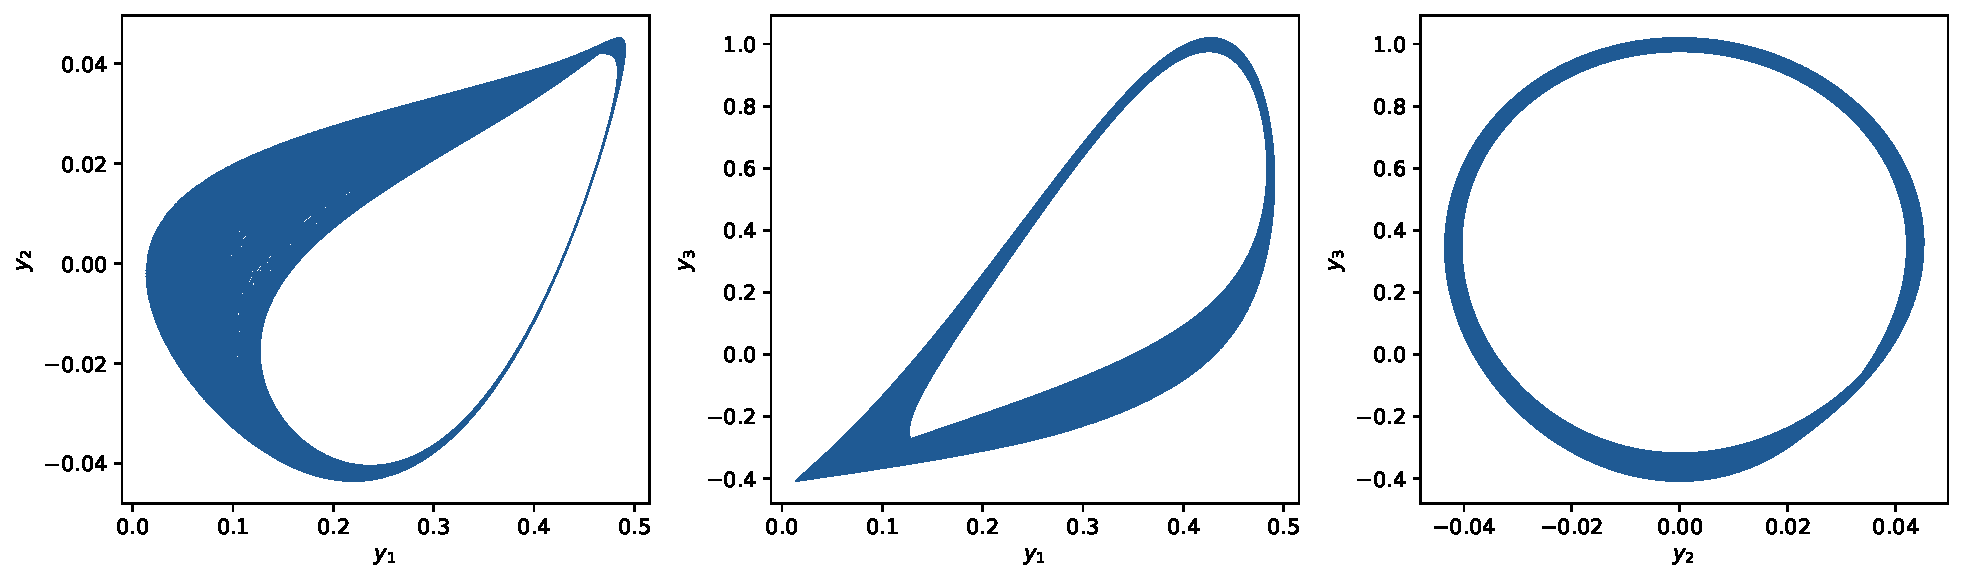
\includegraphics[width=0.94\linewidth,height=0.37\textheight,keepaspectratio]{figures/mavpd_chaos/04_candidate_phase_portraits.pdf}\\[-0.25em]
{\footnotesize MAVPD: proyecciones del candidato caótico.}
\end{center}
\vfill
\begin{center}
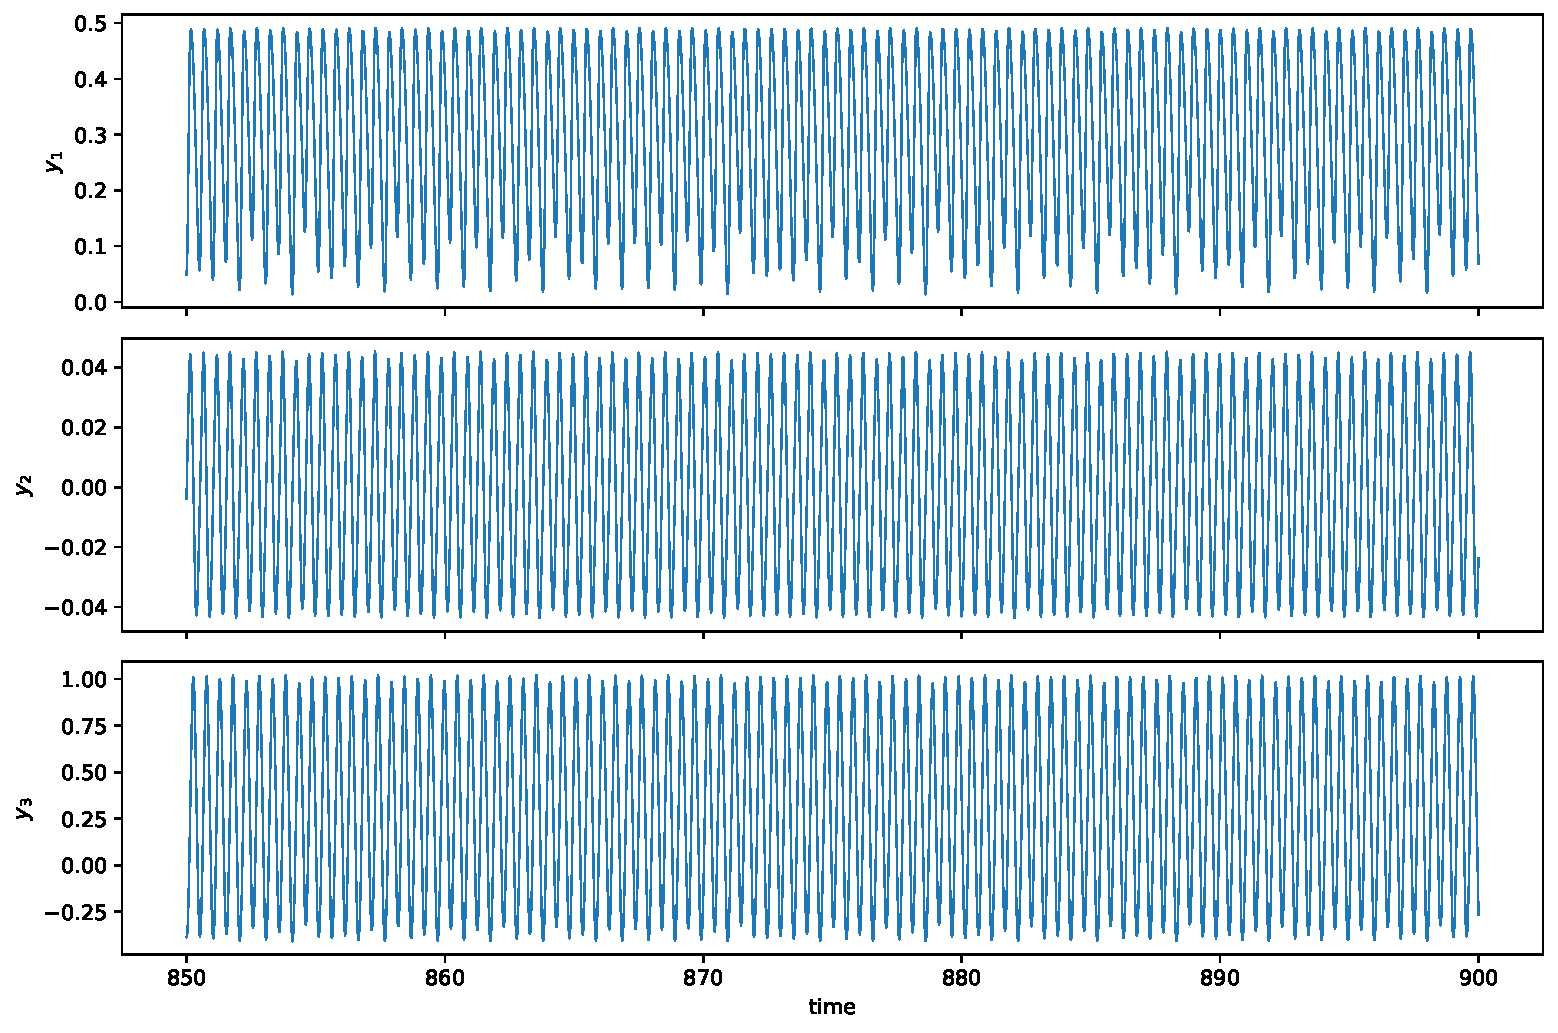
\includegraphics[width=0.94\linewidth,height=0.37\textheight,keepaspectratio]{figures/mavpd_chaos/04_candidate_time_series.pdf}\\[-0.25em]
{\footnotesize MAVPD: series temporales del candidato caótico.}
\end{center}
\clearpage
\begin{center}
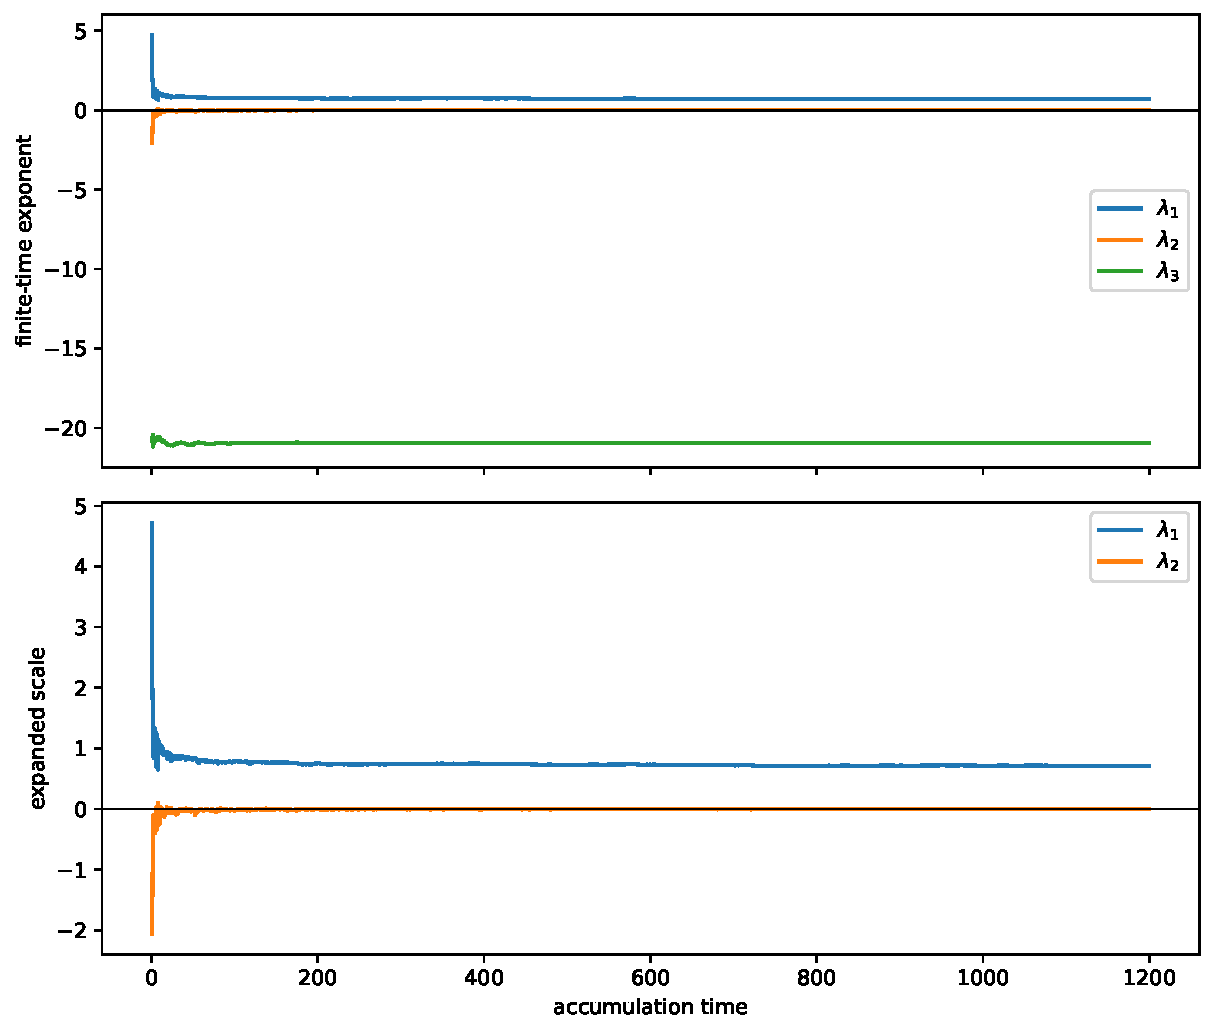
\includegraphics[width=0.94\linewidth,height=0.37\textheight,keepaspectratio]{figures/mavpd_chaos/05_lyapunov_convergence.pdf}\\[-0.25em]
{\footnotesize MAVPD: evolución de las estimaciones de Lyapunov.}
\end{center}
\vfill
\begin{center}
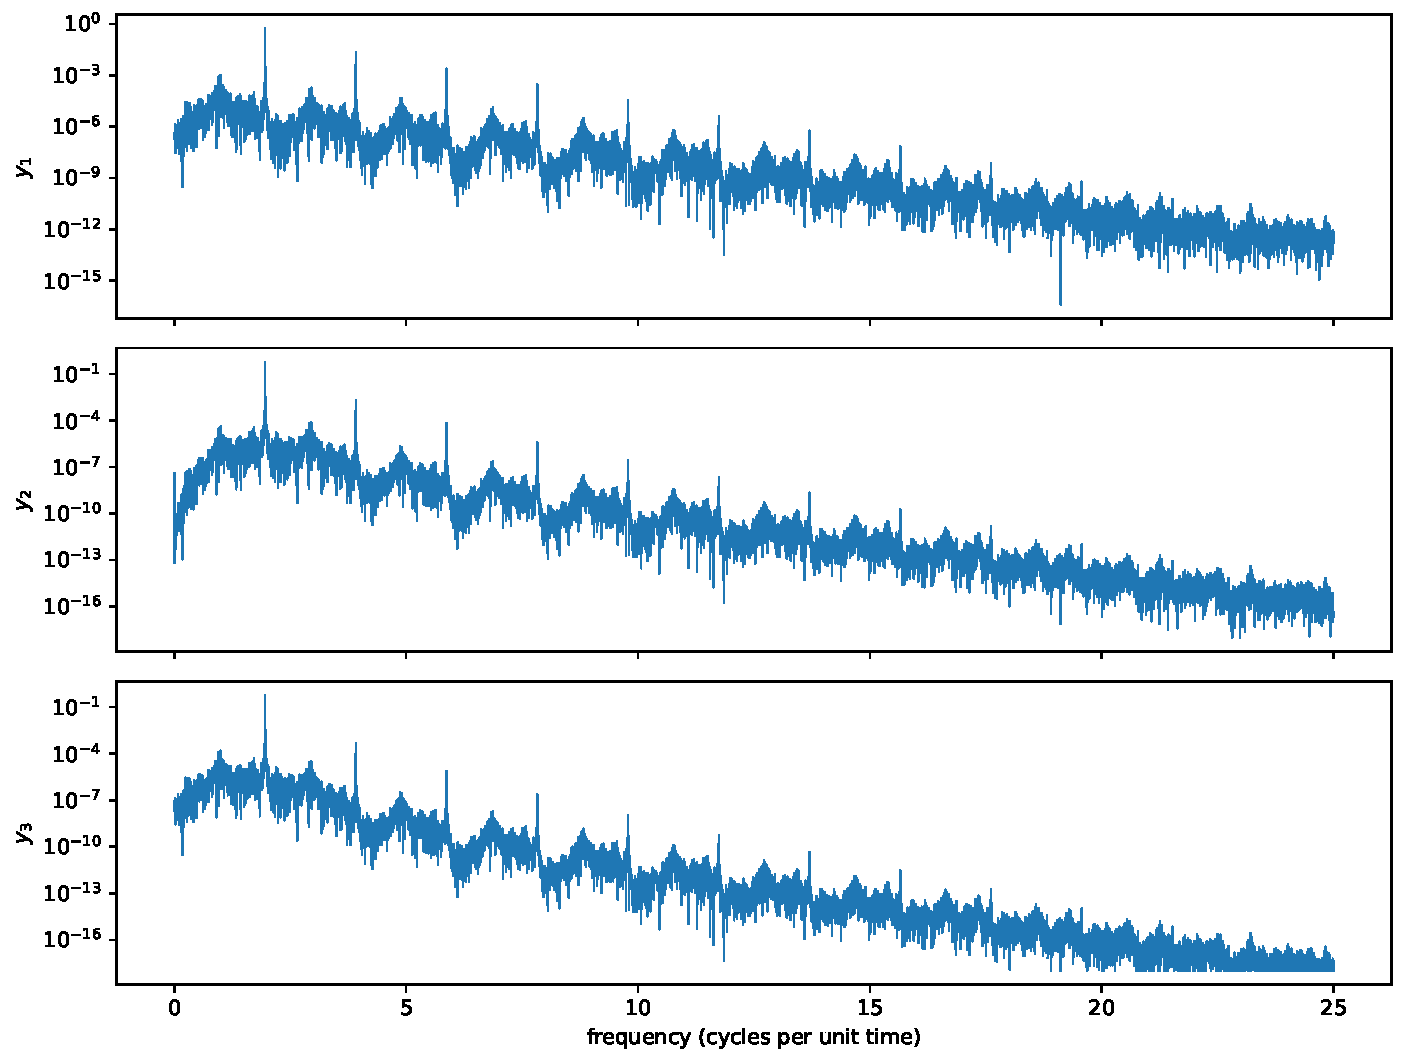
\includegraphics[width=0.94\linewidth,height=0.37\textheight,keepaspectratio]{figures/mavpd_chaos/05_normalized_fft_power.pdf}\\[-0.25em]
{\footnotesize MAVPD: espectro normalizado de la señal.}
\end{center}
\clearpage
\begin{center}
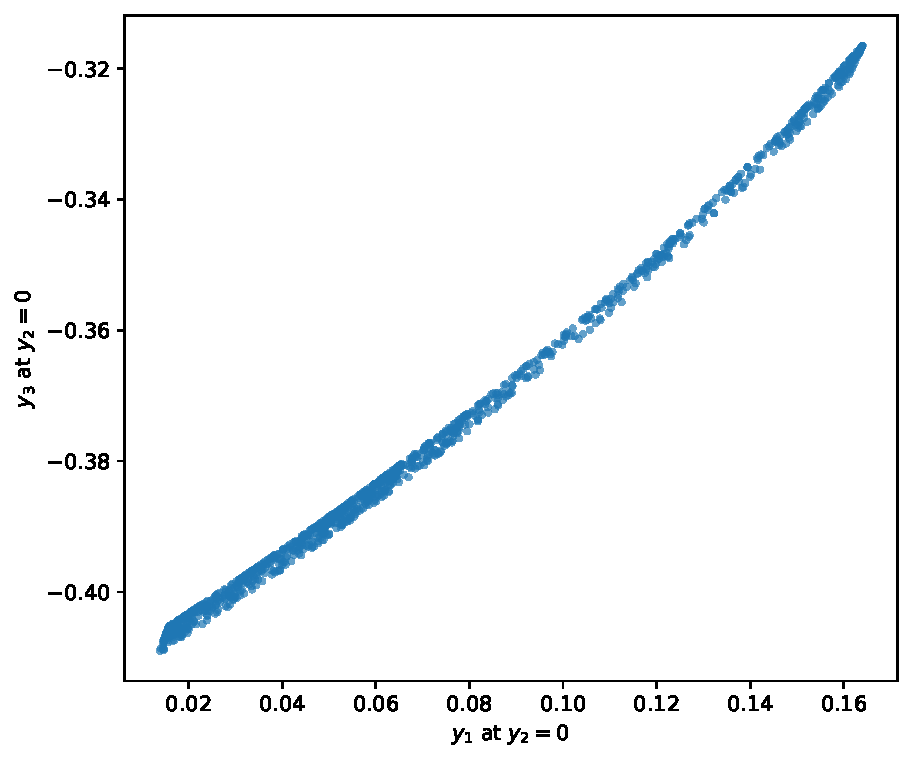
\includegraphics[width=0.94\linewidth,height=0.37\textheight,keepaspectratio]{figures/mavpd_chaos/05_poincare_section.pdf}\\[-0.25em]
{\footnotesize MAVPD: sección de Poincaré del candidato caótico.}
\end{center}
\vfill
\begin{center}
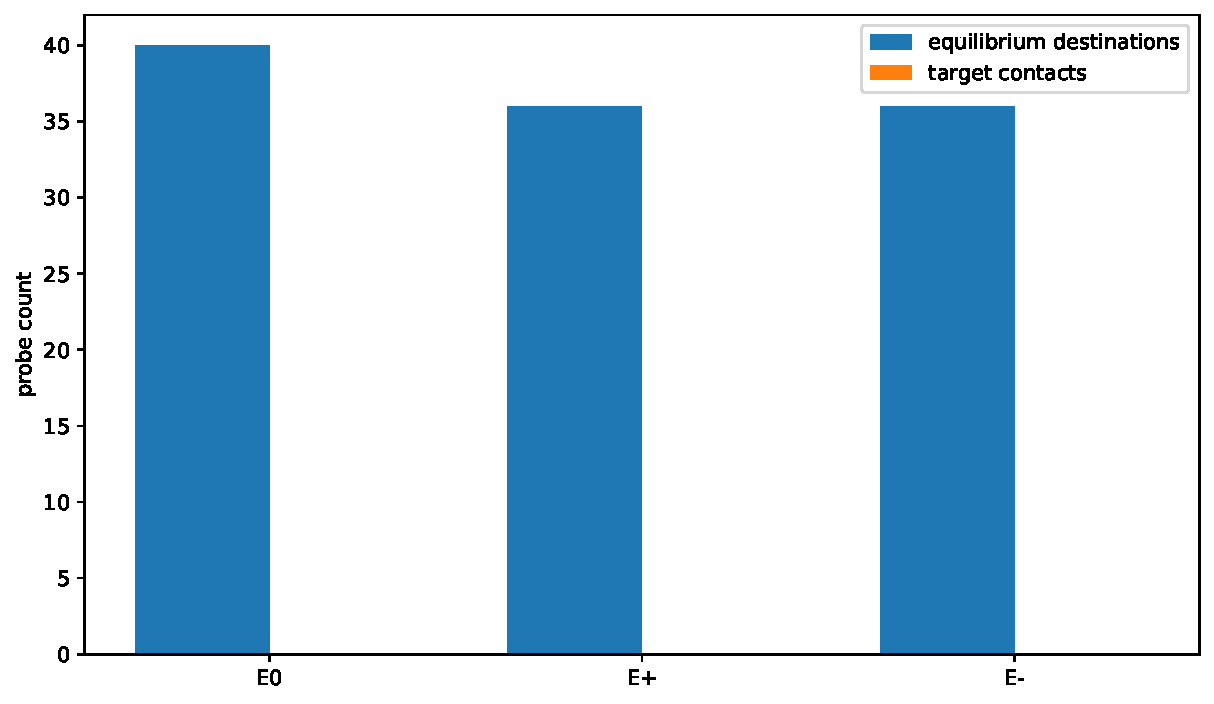
\includegraphics[width=0.94\linewidth,height=0.37\textheight,keepaspectratio]{figures/mavpd_chaos/07_hiddenness_outcomes.pdf}\\[-0.25em]
{\footnotesize MAVPD: destinos de los sondeos próximos a los equilibrios.}
\end{center}
\clearpage
\clearpage
\subsection{PLL lead--lag entero}
Obstrucción de transferencia, continuación en ganancia, ciclos sobre el cilindro y sondeos cilíndricos.

\begin{center}
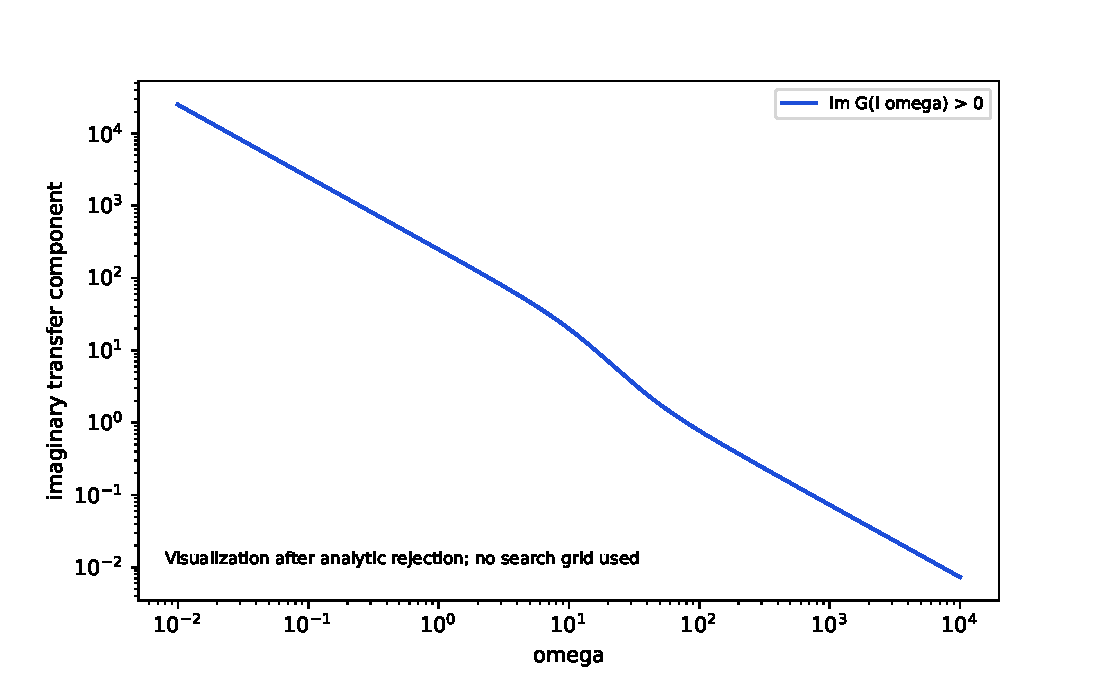
\includegraphics[width=0.94\linewidth,height=0.37\textheight,keepaspectratio]{figures/pll/01_direct_transfer_obstruction.pdf}\\[-0.25em]
{\footnotesize PLL: obstrucción del cierre de transferencia directo.}
\end{center}
\vfill
\begin{center}
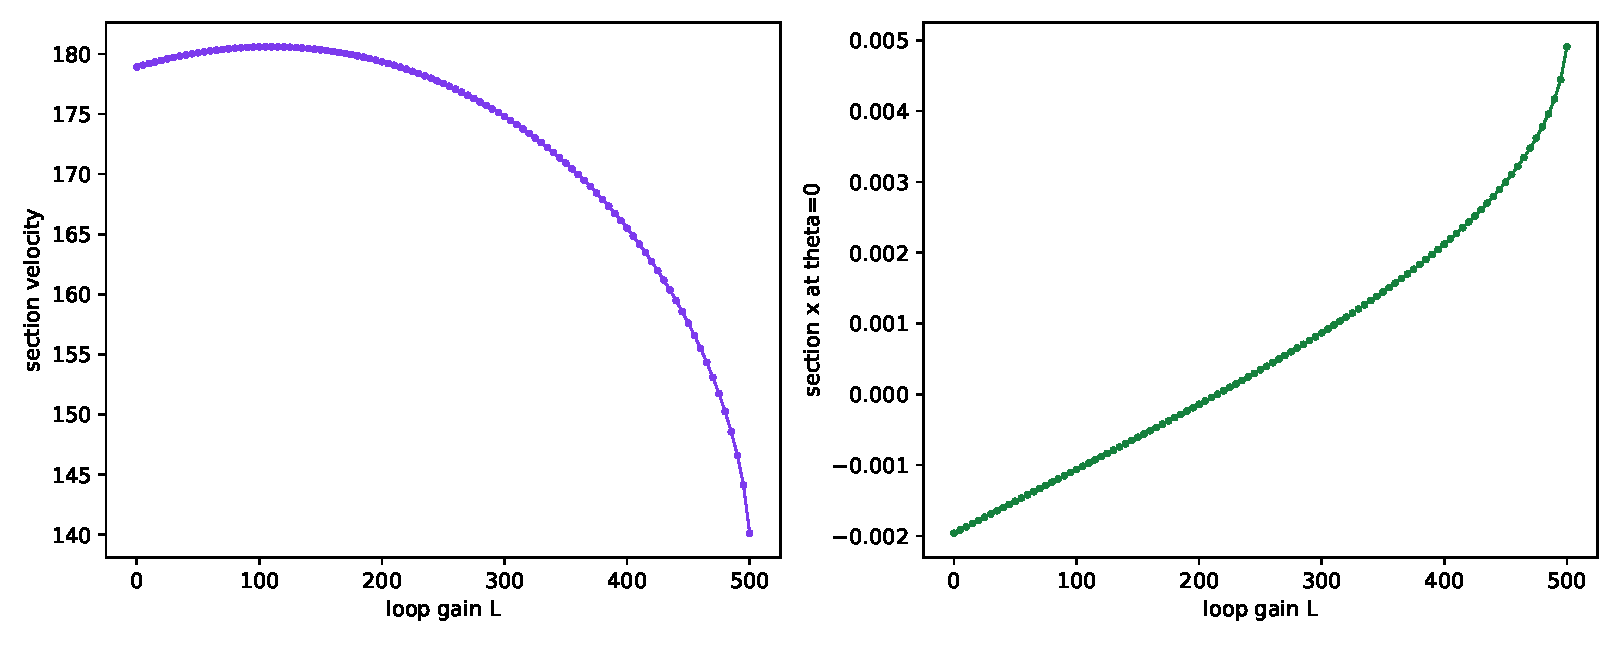
\includegraphics[width=0.94\linewidth,height=0.37\textheight,keepaspectratio]{figures/pll/02_loop_gain_continuation.pdf}\\[-0.25em]
{\footnotesize PLL: continuación de la ganancia de lazo.}
\end{center}
\clearpage
\begin{center}
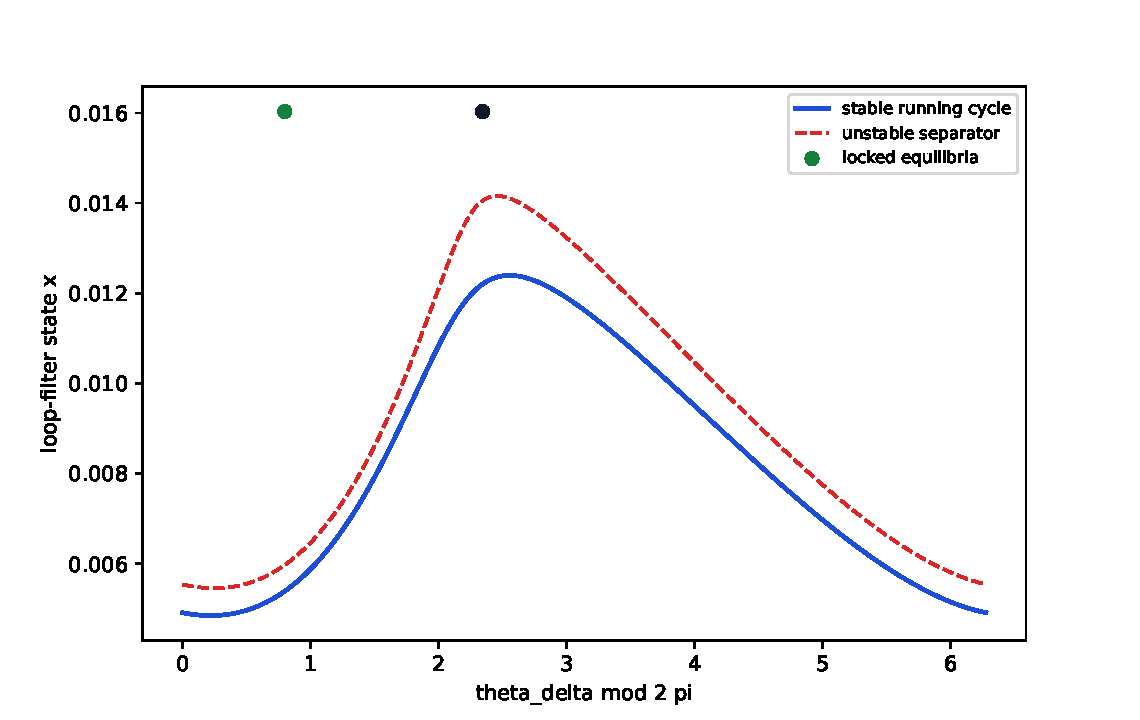
\includegraphics[width=0.94\linewidth,height=0.37\textheight,keepaspectratio]{figures/pll/03_phase_cylinder_cycles.pdf}\\[-0.25em]
{\footnotesize PLL: órbitas sobre el cilindro de fases.}
\end{center}
\vfill
\begin{center}
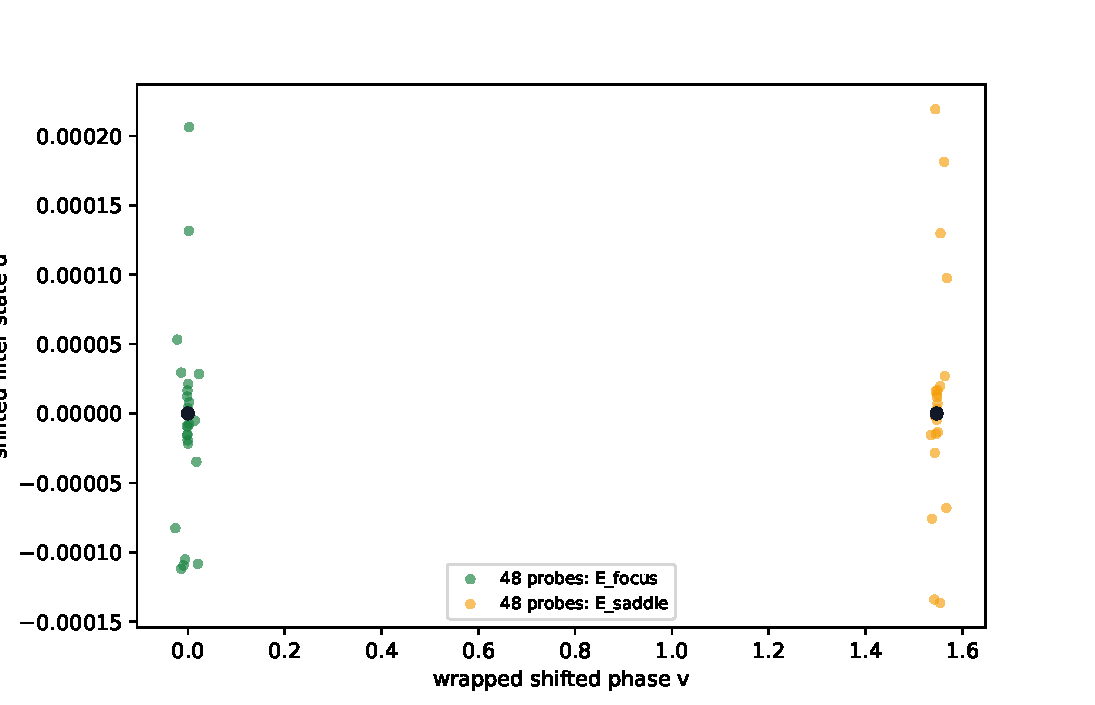
\includegraphics[width=0.94\linewidth,height=0.37\textheight,keepaspectratio]{figures/pll/04_cylindrical_hiddenness_probes.pdf}\\[-0.25em]
{\footnotesize PLL: sondeos de cuenca con distancia cilíndrica.}
\end{center}
\clearpage
\clearpage
\subsection{Chua arctangente c590: cortes adicionales de cuenca}
Los cinco cortes utilizan ABM--PECE con memoria completa, $q=0.9999$,
$h=0.005$, horizonte 180 y descarte de 90. La retícula visual de
$241\times241$ nodos por plano representa 62\,416 trayectorias integradas:
35\,941 de una malla de base y 26\,475 centros de celdas con clases
heterogéneas. Los demás nodos reciben relleno categórico; los 290\,405
nodos visibles no son integraciones independientes. El gris incluye
salidas detectadas y puntos omitidos en la malla de base, por lo que no
acredita una salida calculada en cada píxel.
Los colores distinguen contacto con $A_\pm$, proximidad a $E_0,E_\pm$,
otro destino acotado o salida según el clasificador finito. No determinan
por sí solos cuencas asintóticas ni fracciones de volumen.
Las estrellas marcan equilibrios contenidos en el plano y los círculos,
sus proyecciones desde otros planos.

\begin{center}
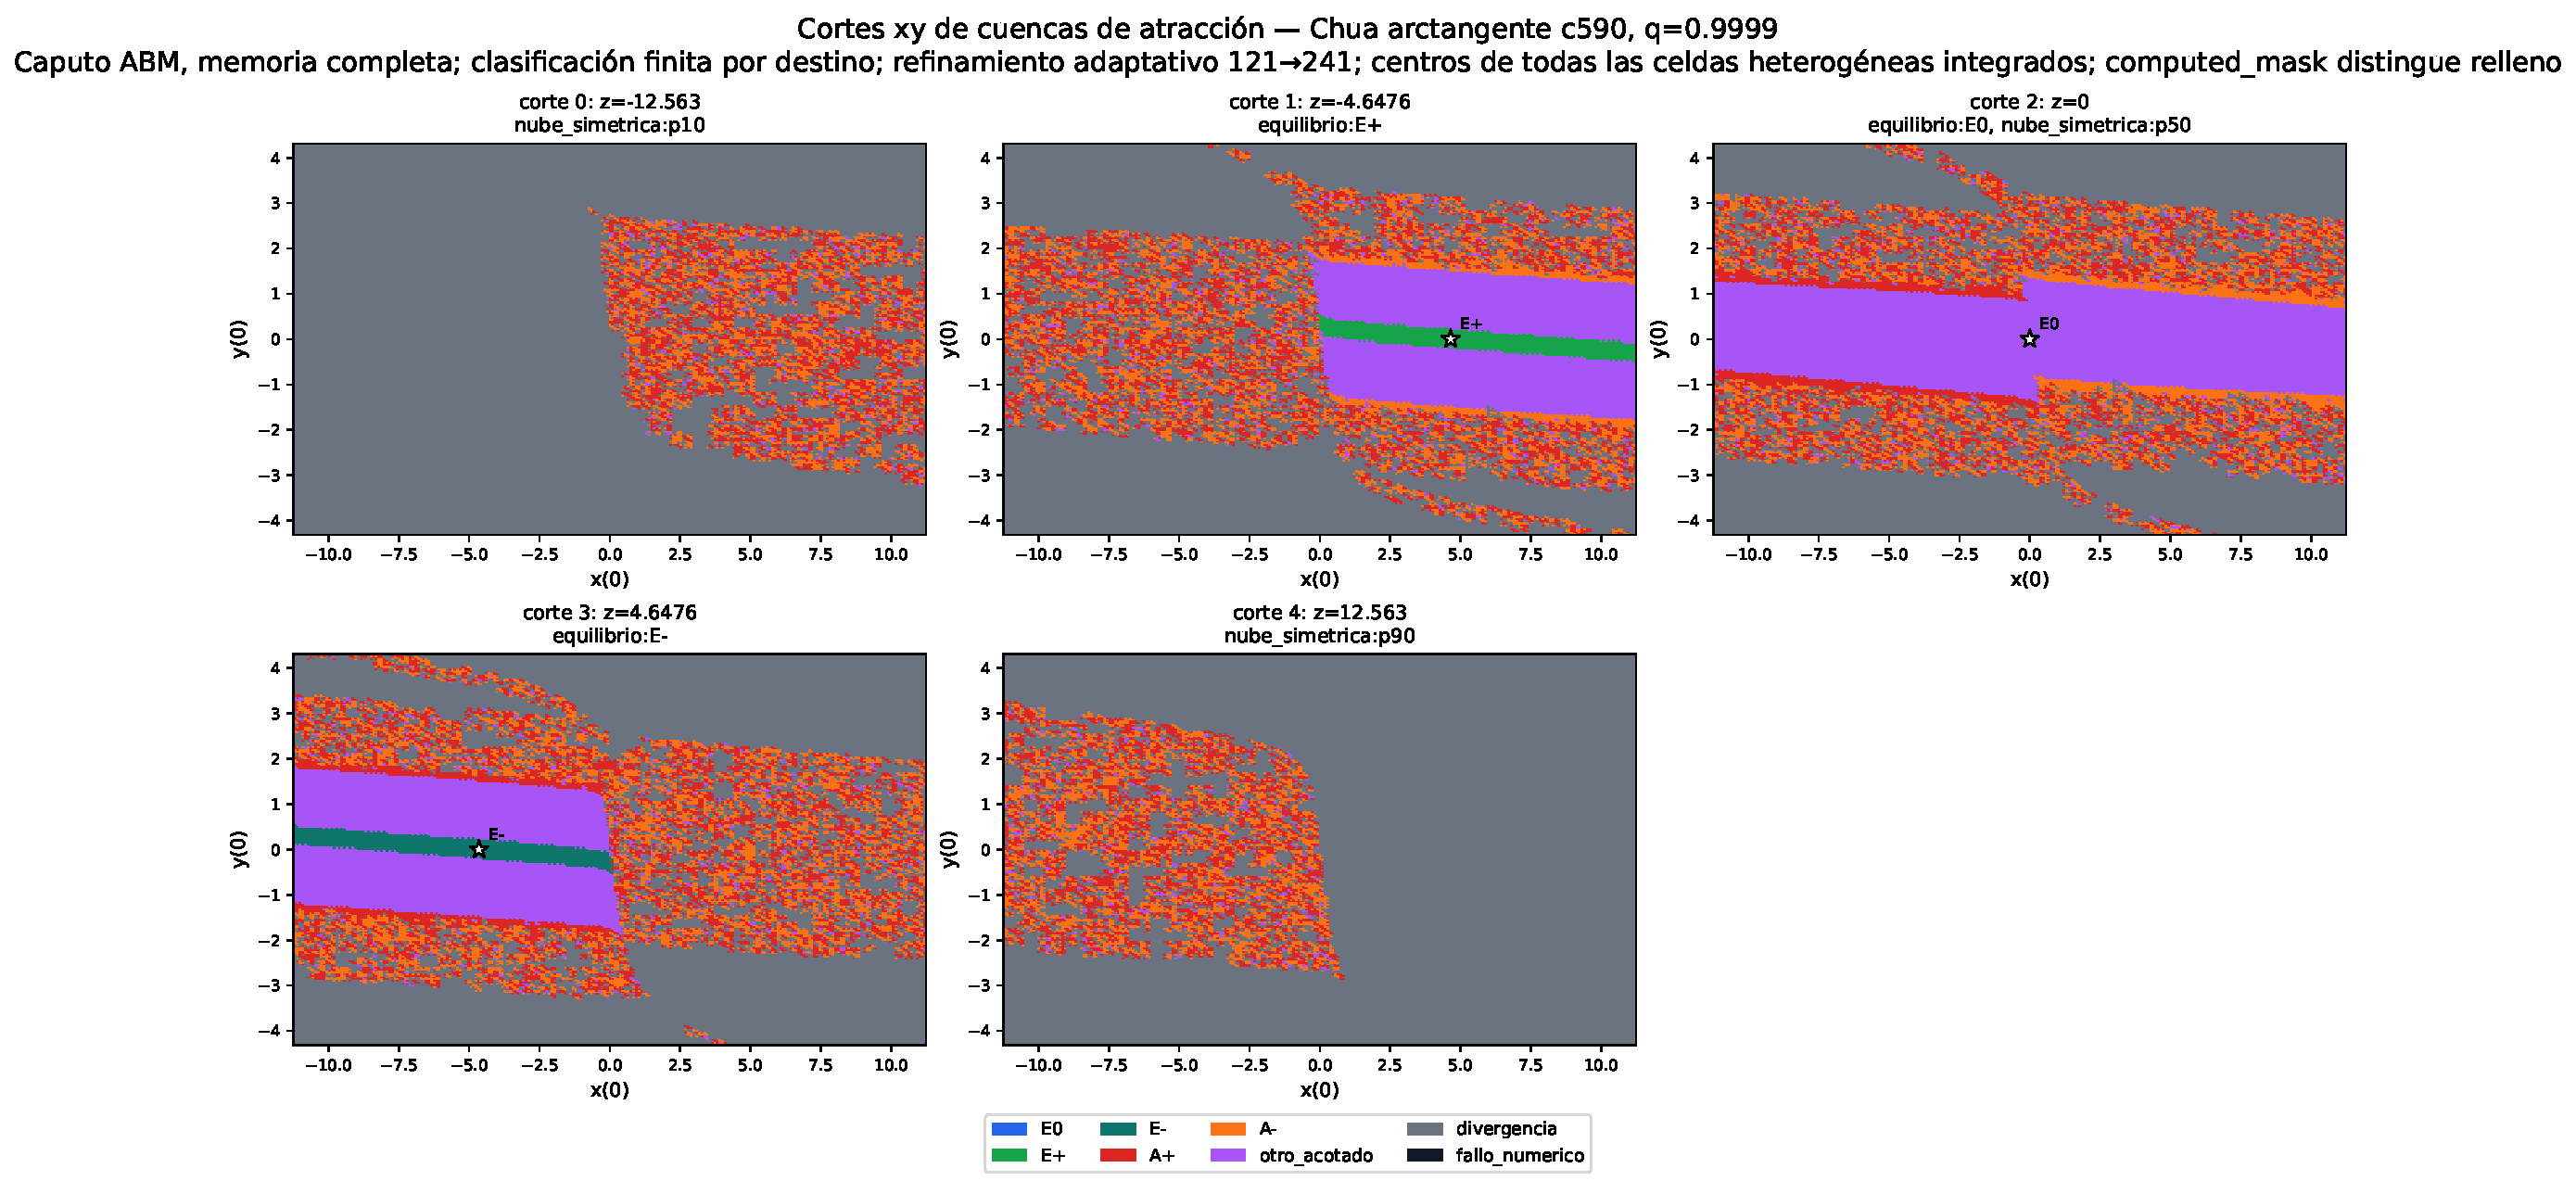
\includegraphics[width=0.94\linewidth,height=0.37\textheight,keepaspectratio]{figures/c590_basin/basin_multislice.pdf}\\[-0.25em]
{\footnotesize Cortes de las regiones de destino.}
\end{center}
\vfill
\begin{center}
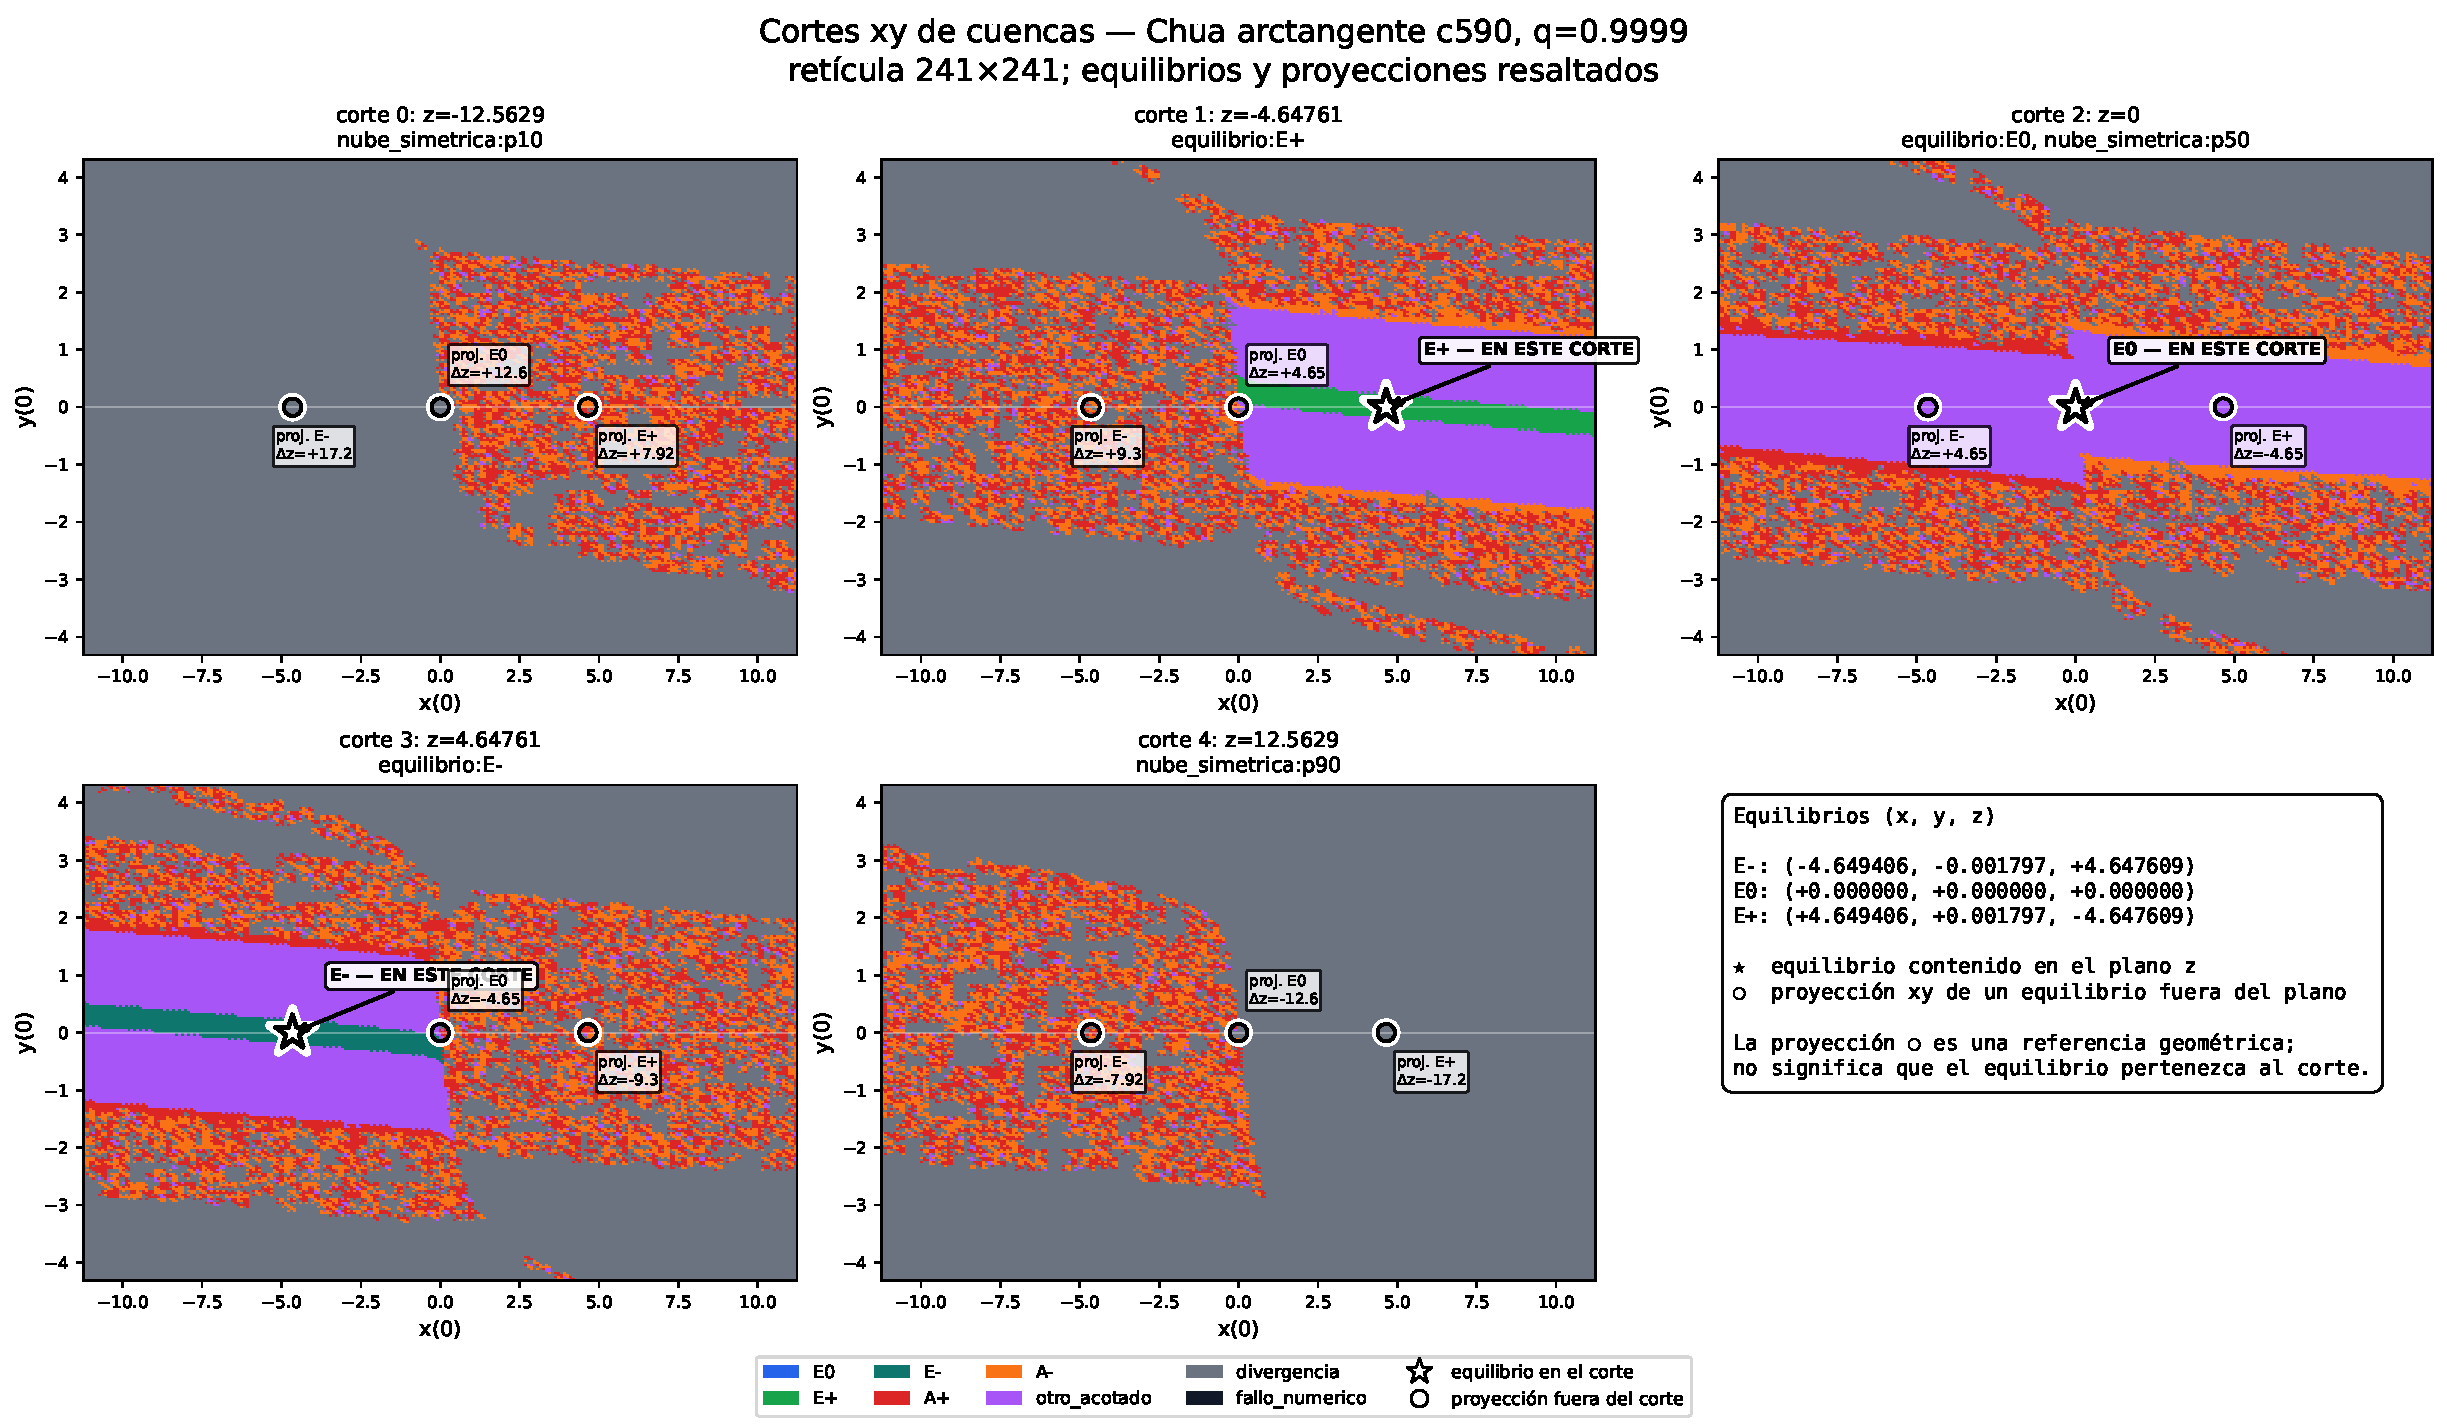
\includegraphics[width=0.94\linewidth,height=0.37\textheight,keepaspectratio]{figures/c590_basin/basin_multislice_equilibria.pdf}\\[-0.25em]
{\footnotesize Cortes de las regiones de destino y posición de los equilibrios.}
\end{center}
\clearpage
\begin{center}
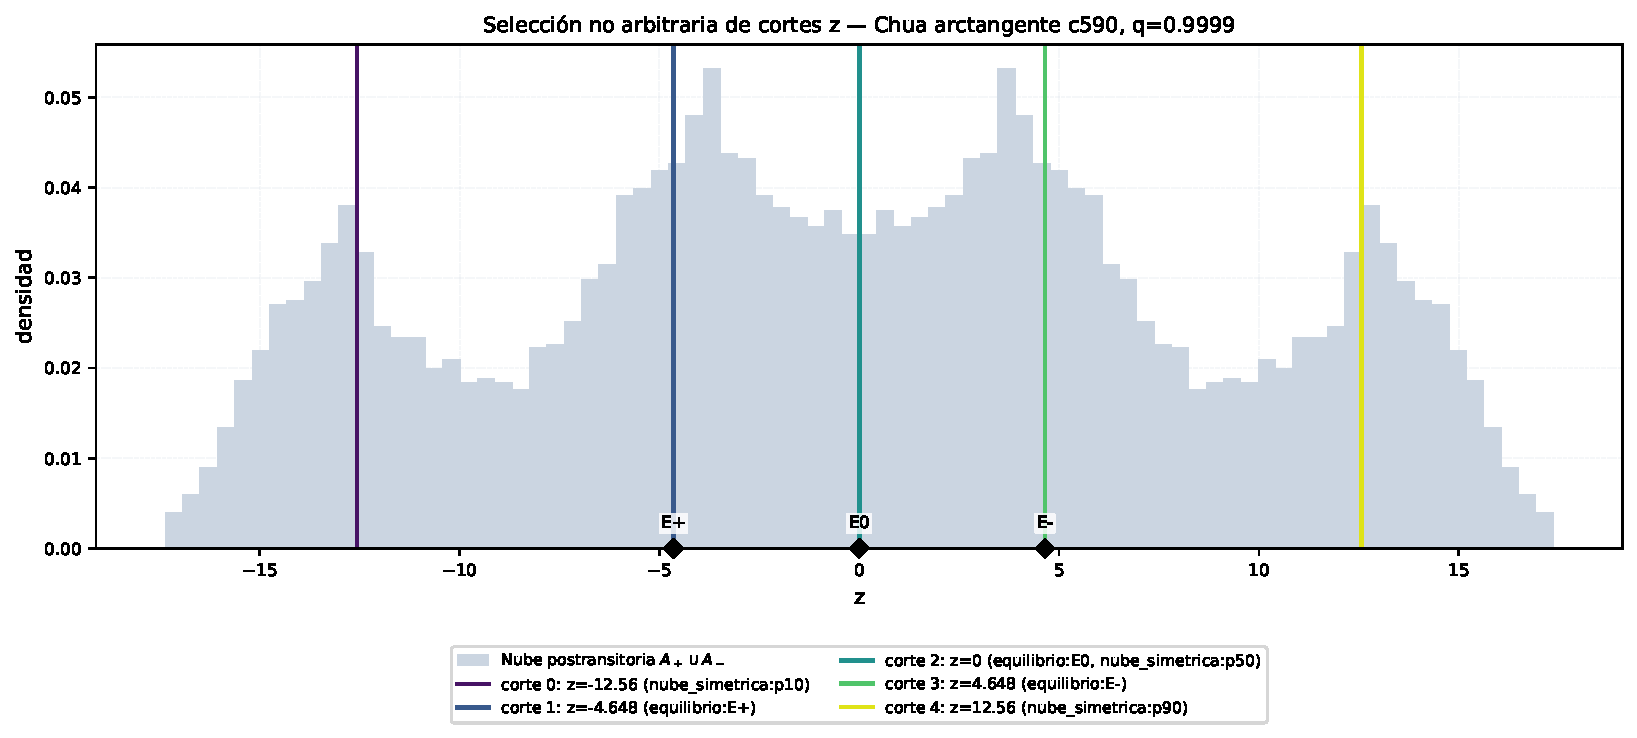
\includegraphics[width=0.94\linewidth,height=0.37\textheight,keepaspectratio]{figures/c590_basin/z_cut_selection.pdf}\\[-0.25em]
{\footnotesize Posición de los planos de corte de las regiones de destino.}
\end{center}
\vfill
\begin{center}
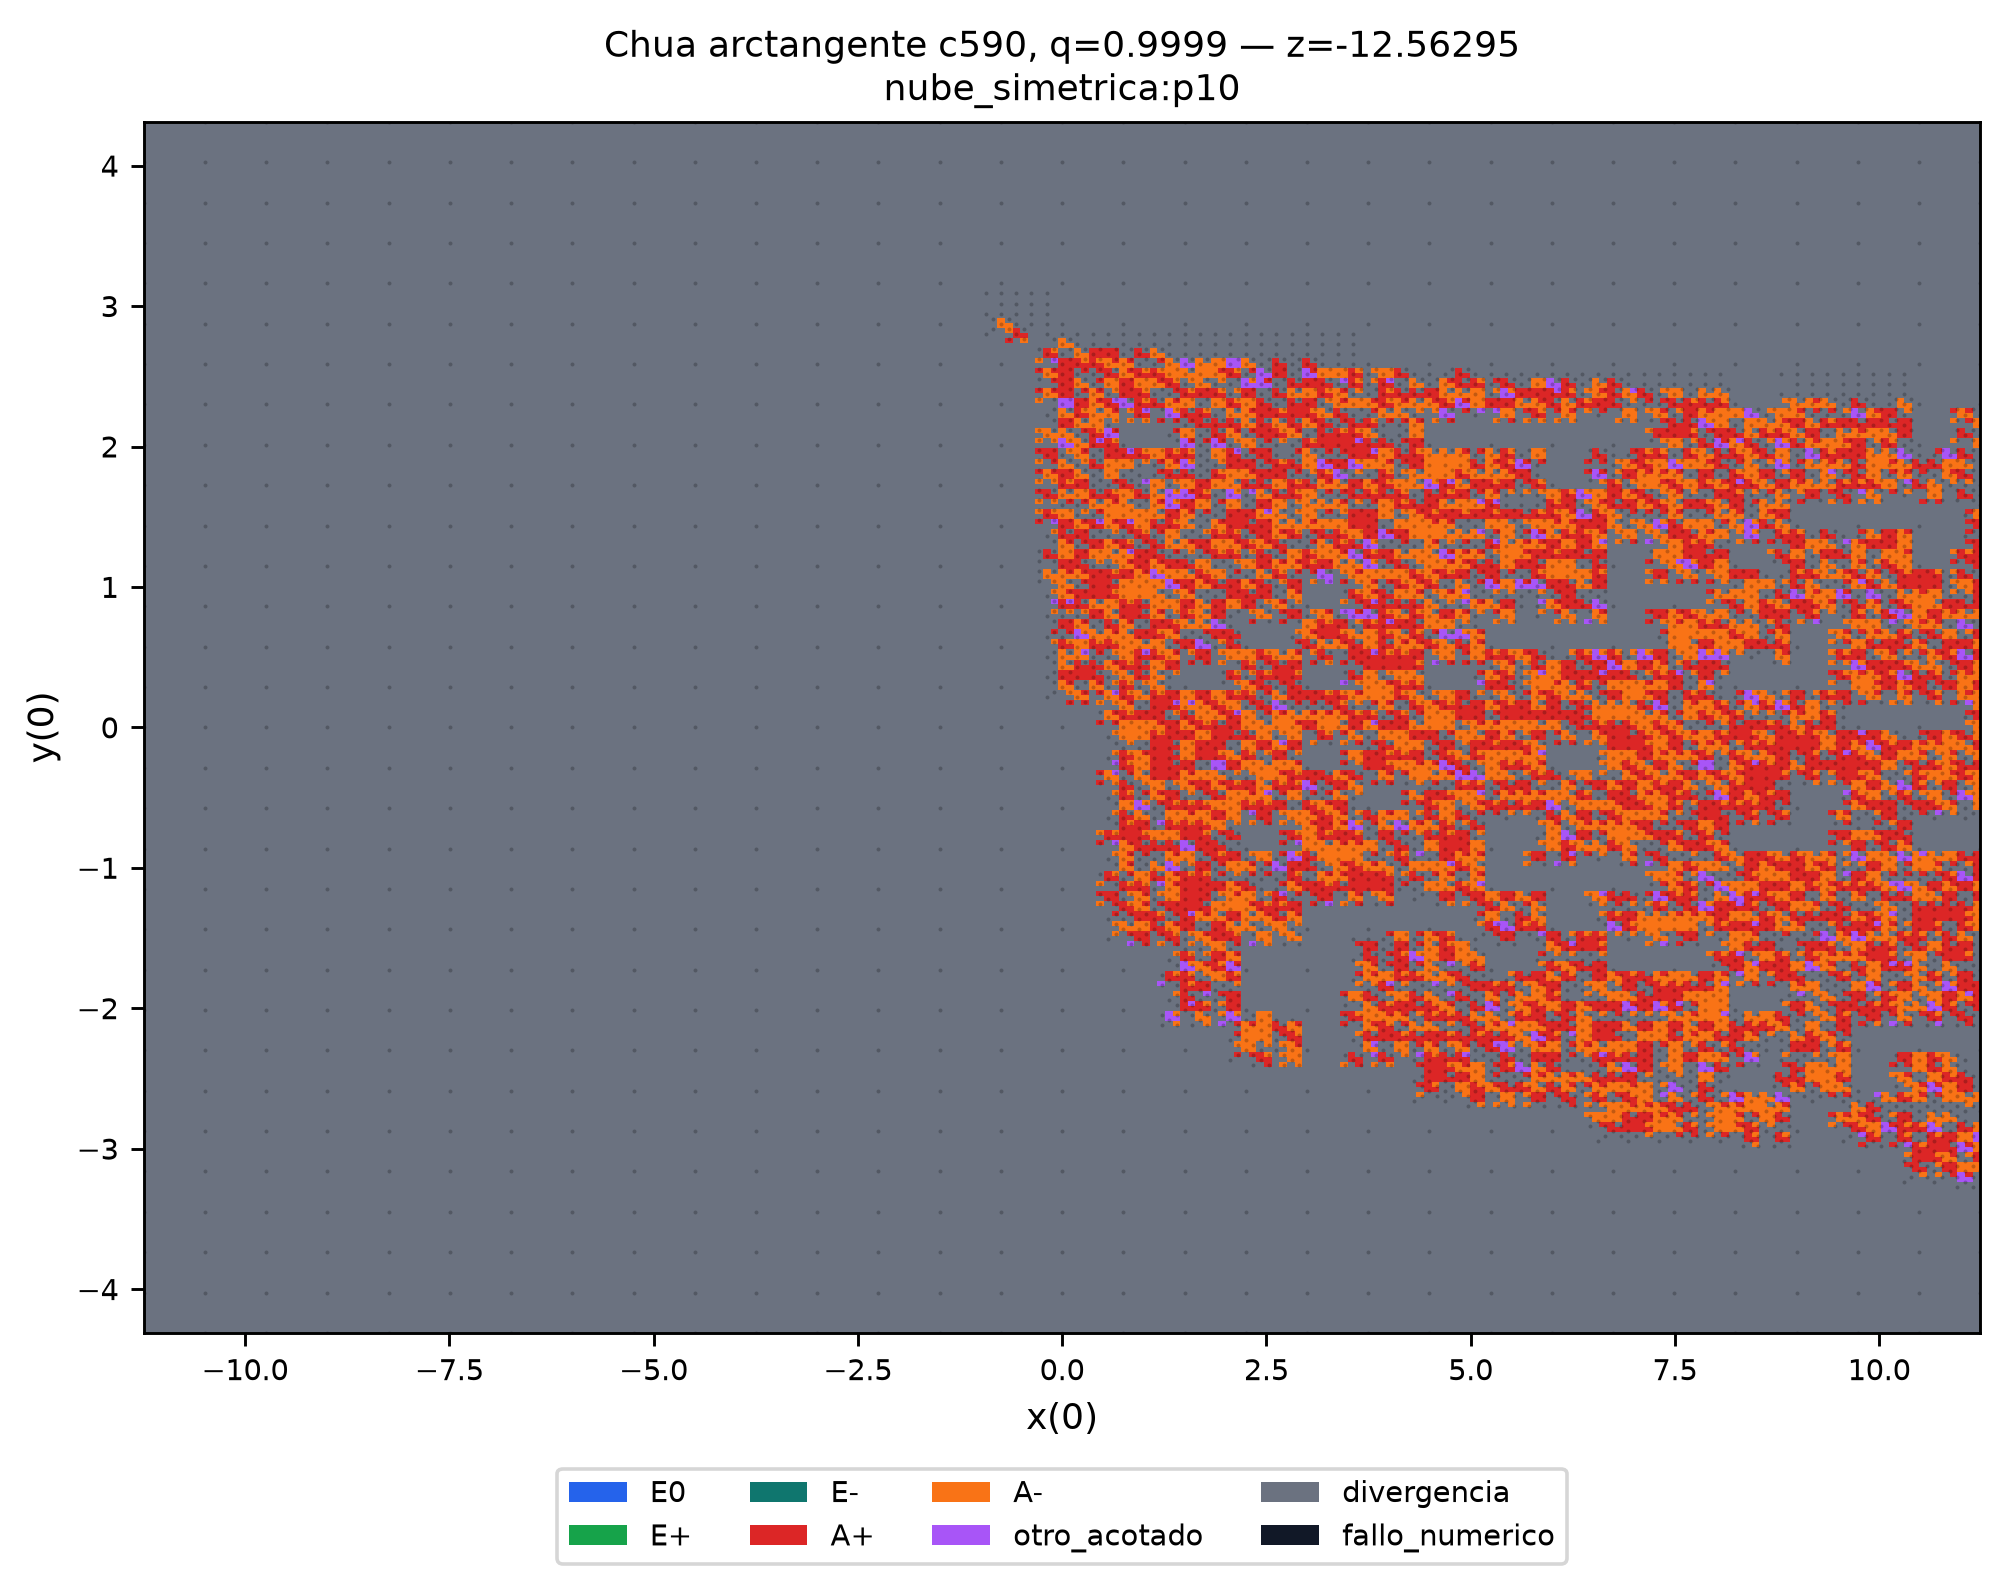
\includegraphics[width=0.94\linewidth,height=0.37\textheight,keepaspectratio]{figures/c590_basin/basin_cut_00.png}\\[-0.25em]
{\footnotesize Corte 1 de las regiones de destino.}
\end{center}
\clearpage
\begin{center}
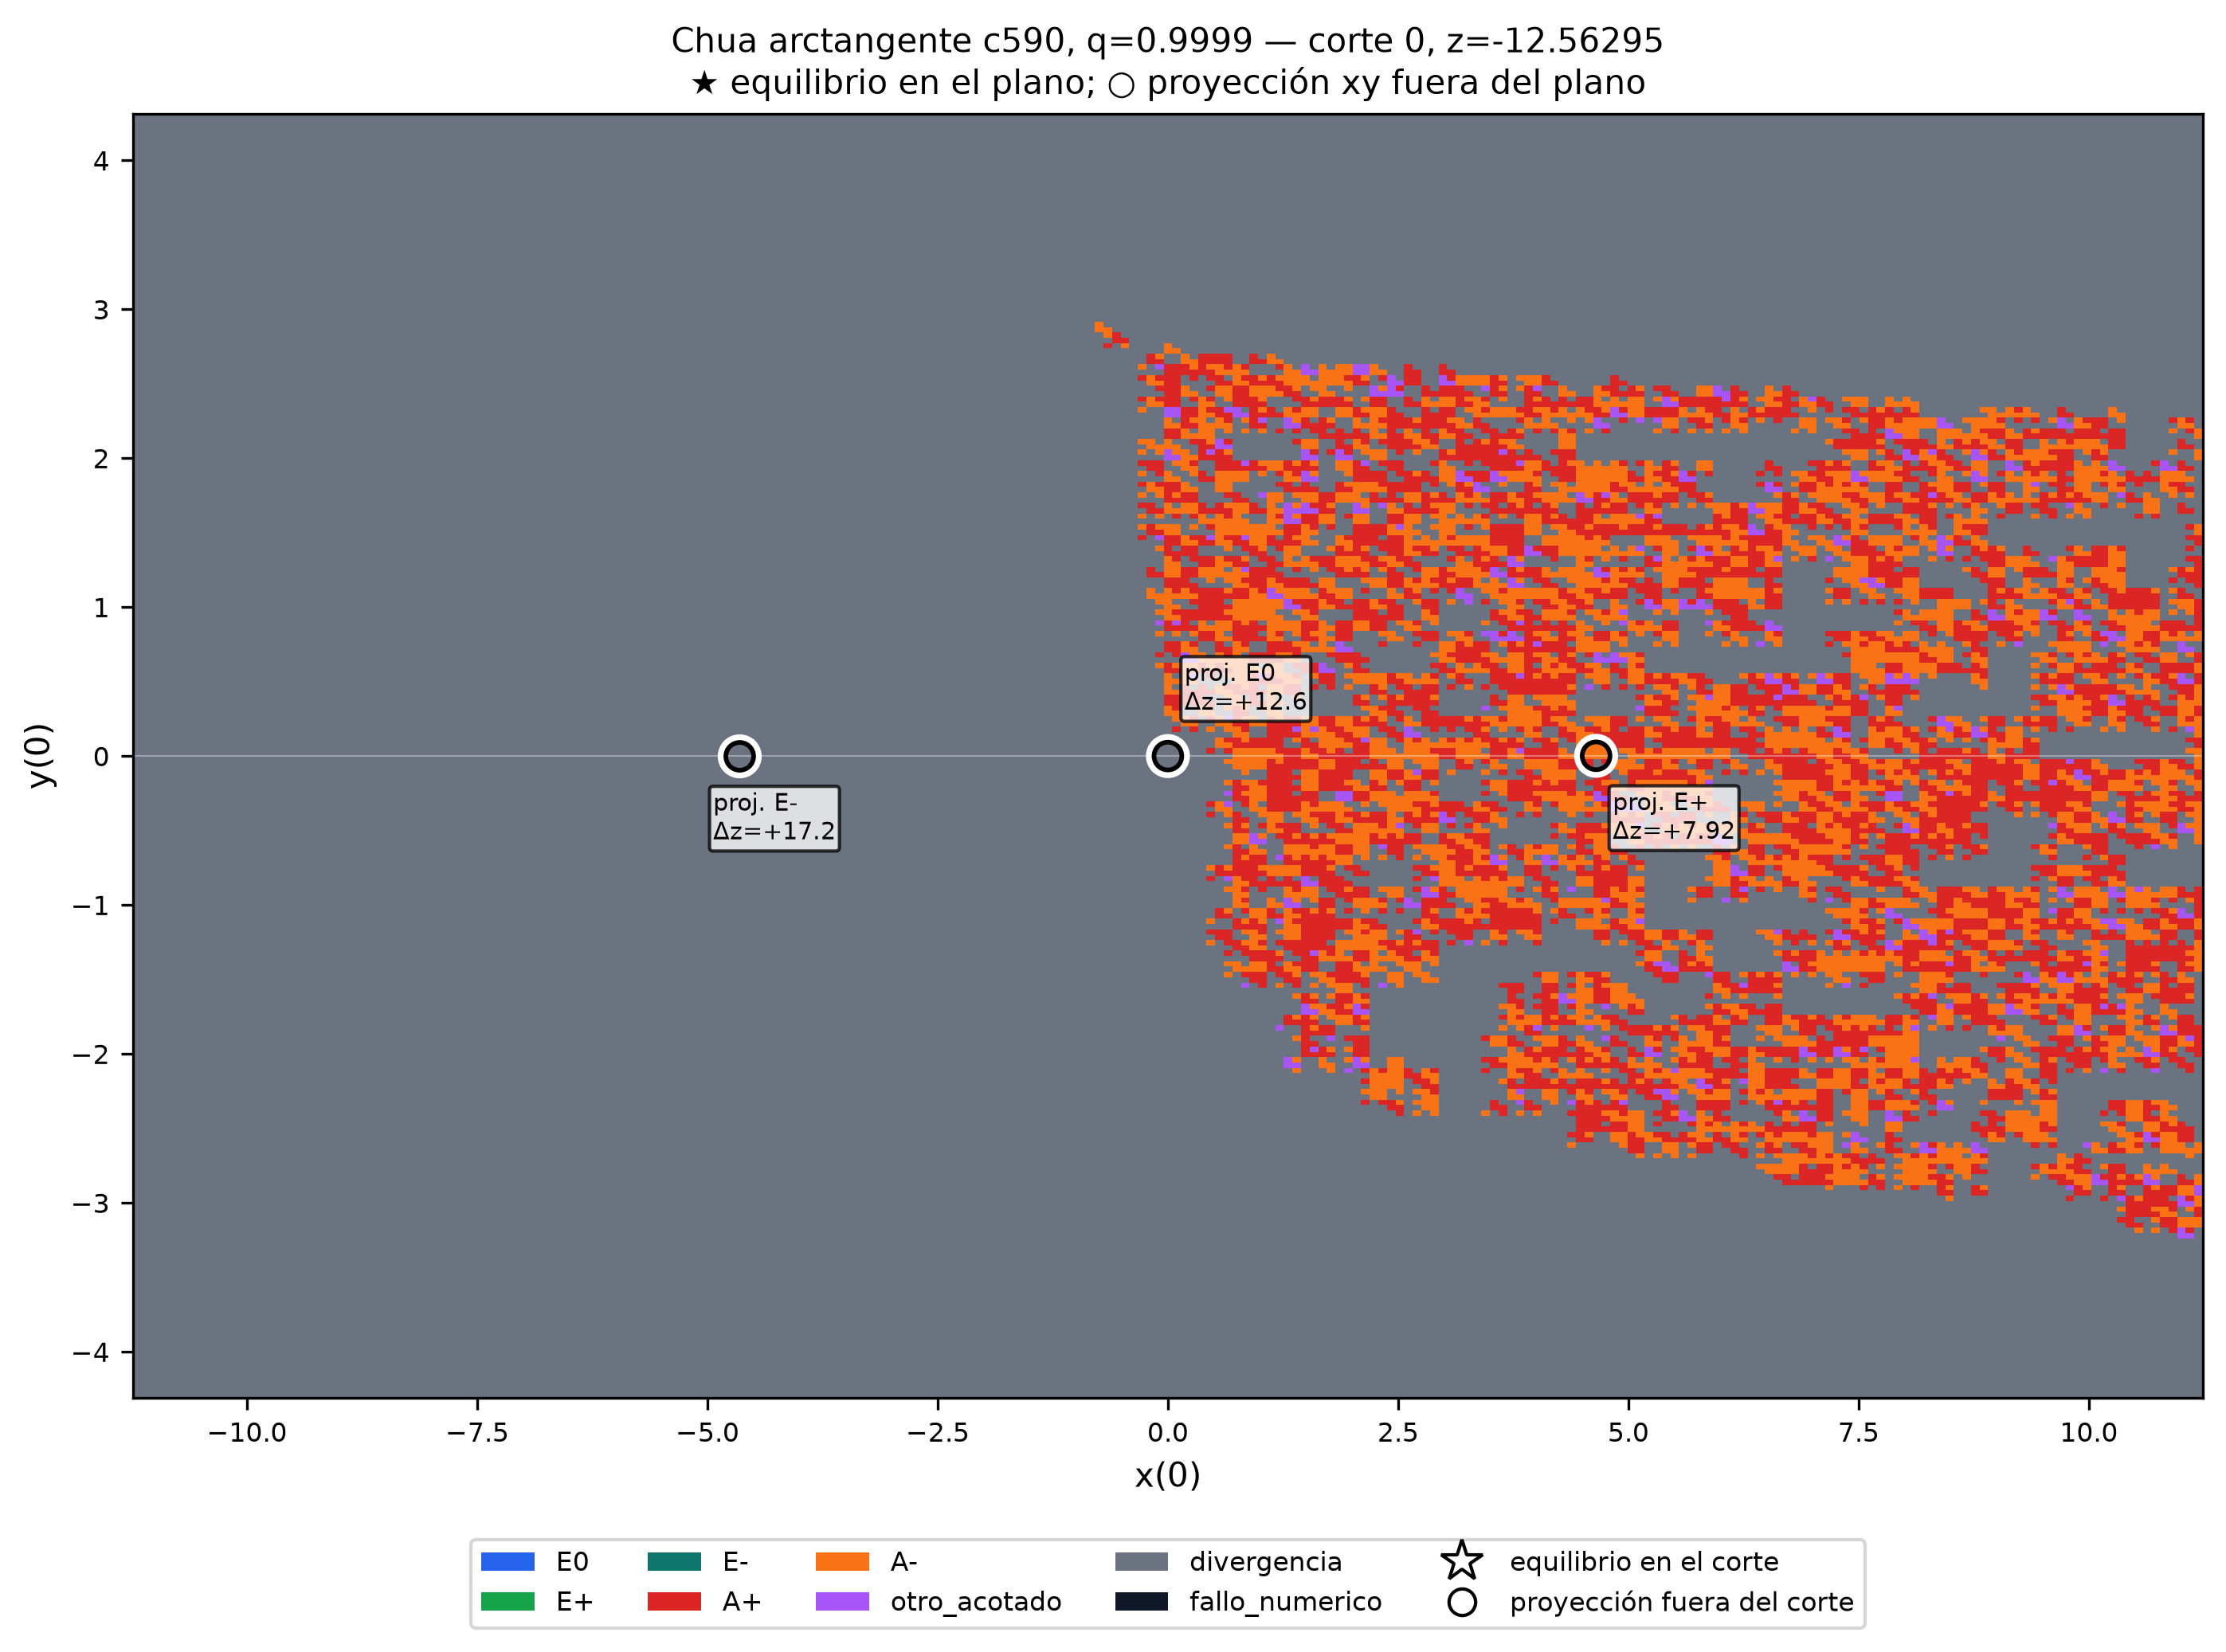
\includegraphics[width=0.94\linewidth,height=0.37\textheight,keepaspectratio]{figures/c590_basin/basin_cut_00_equilibria.png}\\[-0.25em]
{\footnotesize Corte 1 de las regiones de destino y posición de los equilibrios.}
\end{center}
\vfill
\begin{center}
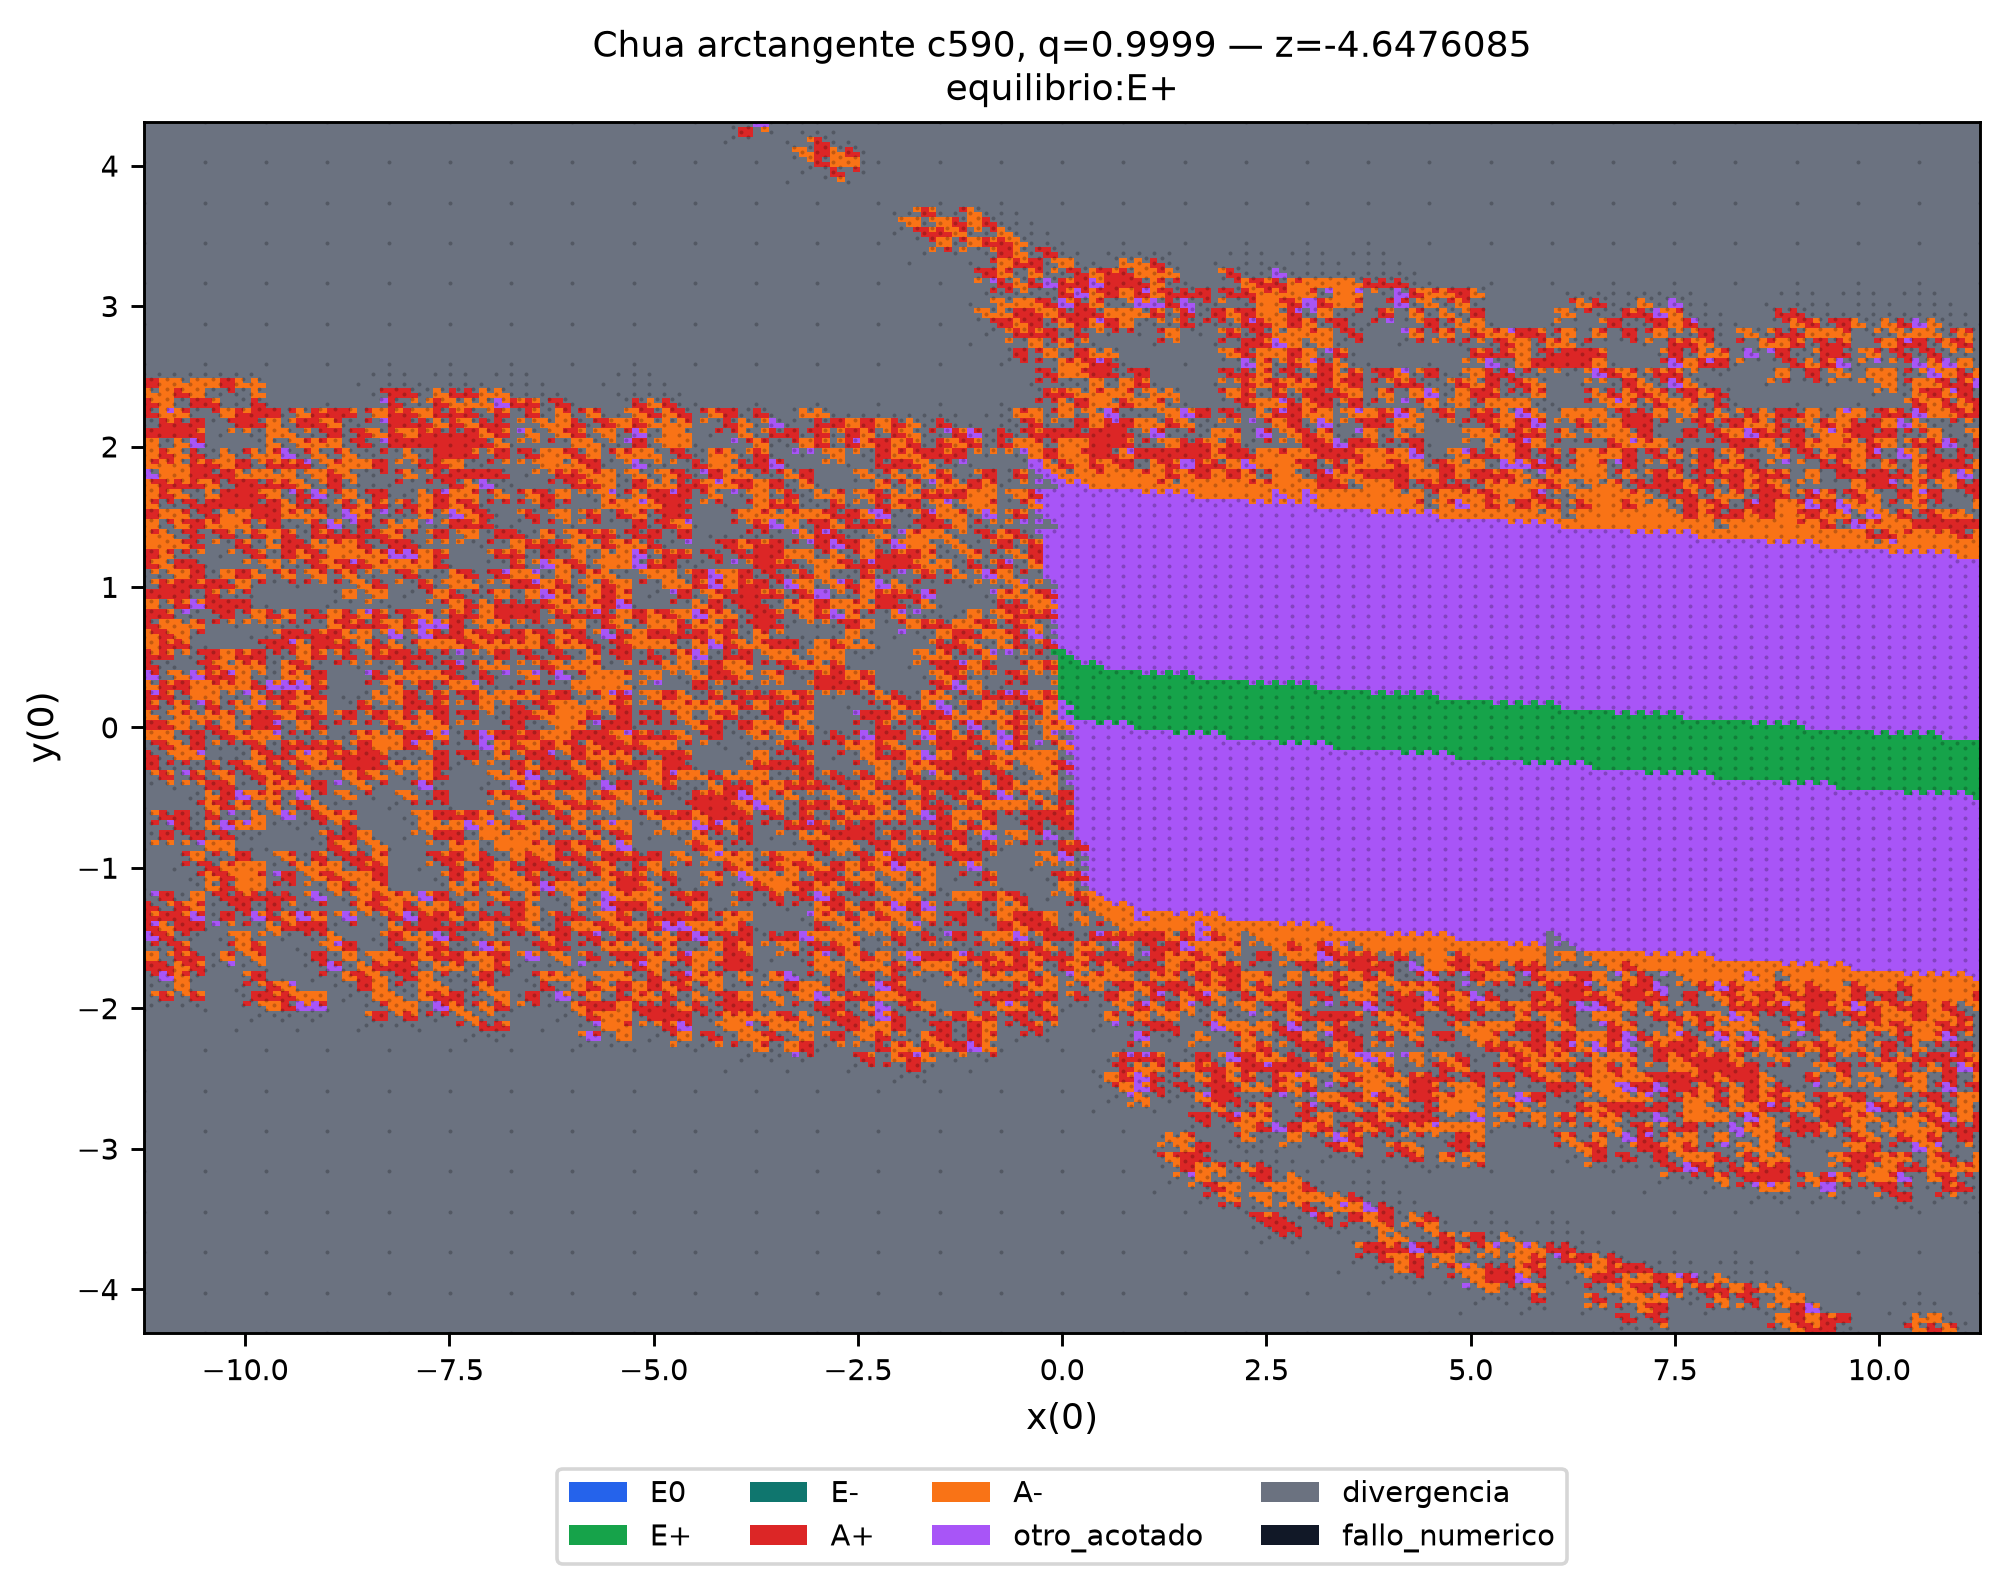
\includegraphics[width=0.94\linewidth,height=0.37\textheight,keepaspectratio]{figures/c590_basin/basin_cut_01.png}\\[-0.25em]
{\footnotesize Corte 2 de las regiones de destino.}
\end{center}
\clearpage
\begin{center}
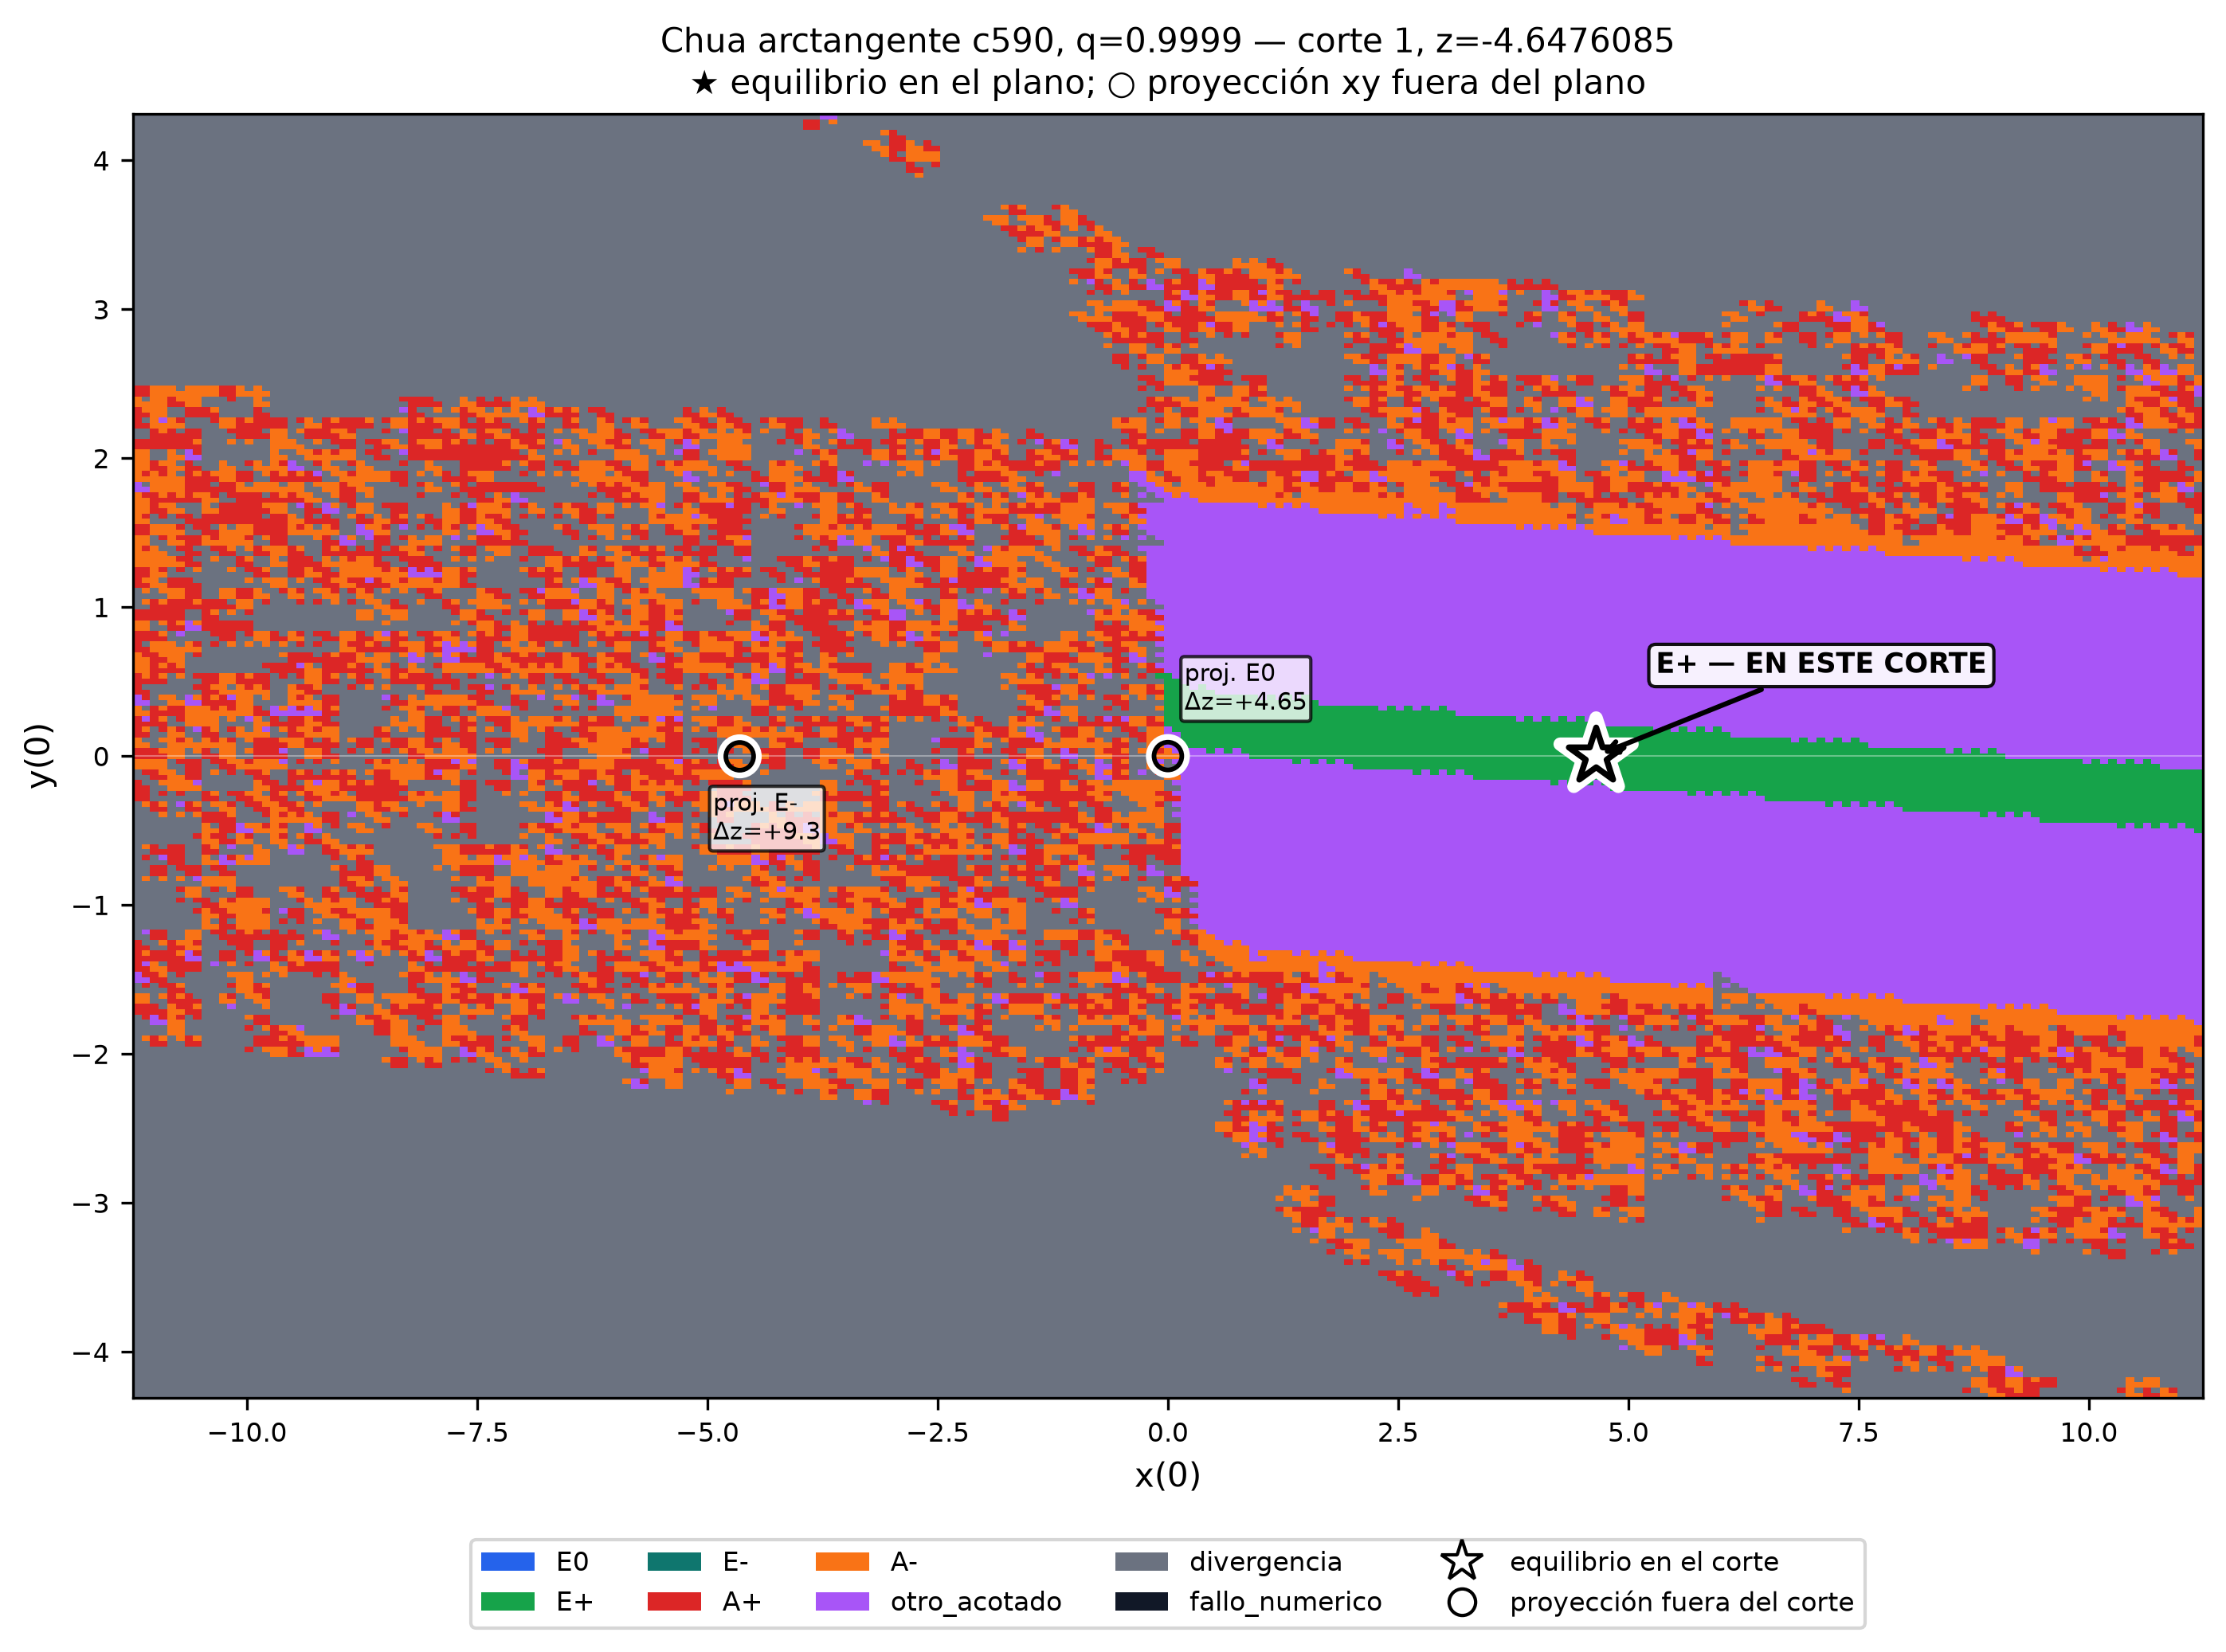
\includegraphics[width=0.94\linewidth,height=0.37\textheight,keepaspectratio]{figures/c590_basin/basin_cut_01_equilibria.png}\\[-0.25em]
{\footnotesize Corte 2 de las regiones de destino y posición de los equilibrios.}
\end{center}
\vfill
\begin{center}
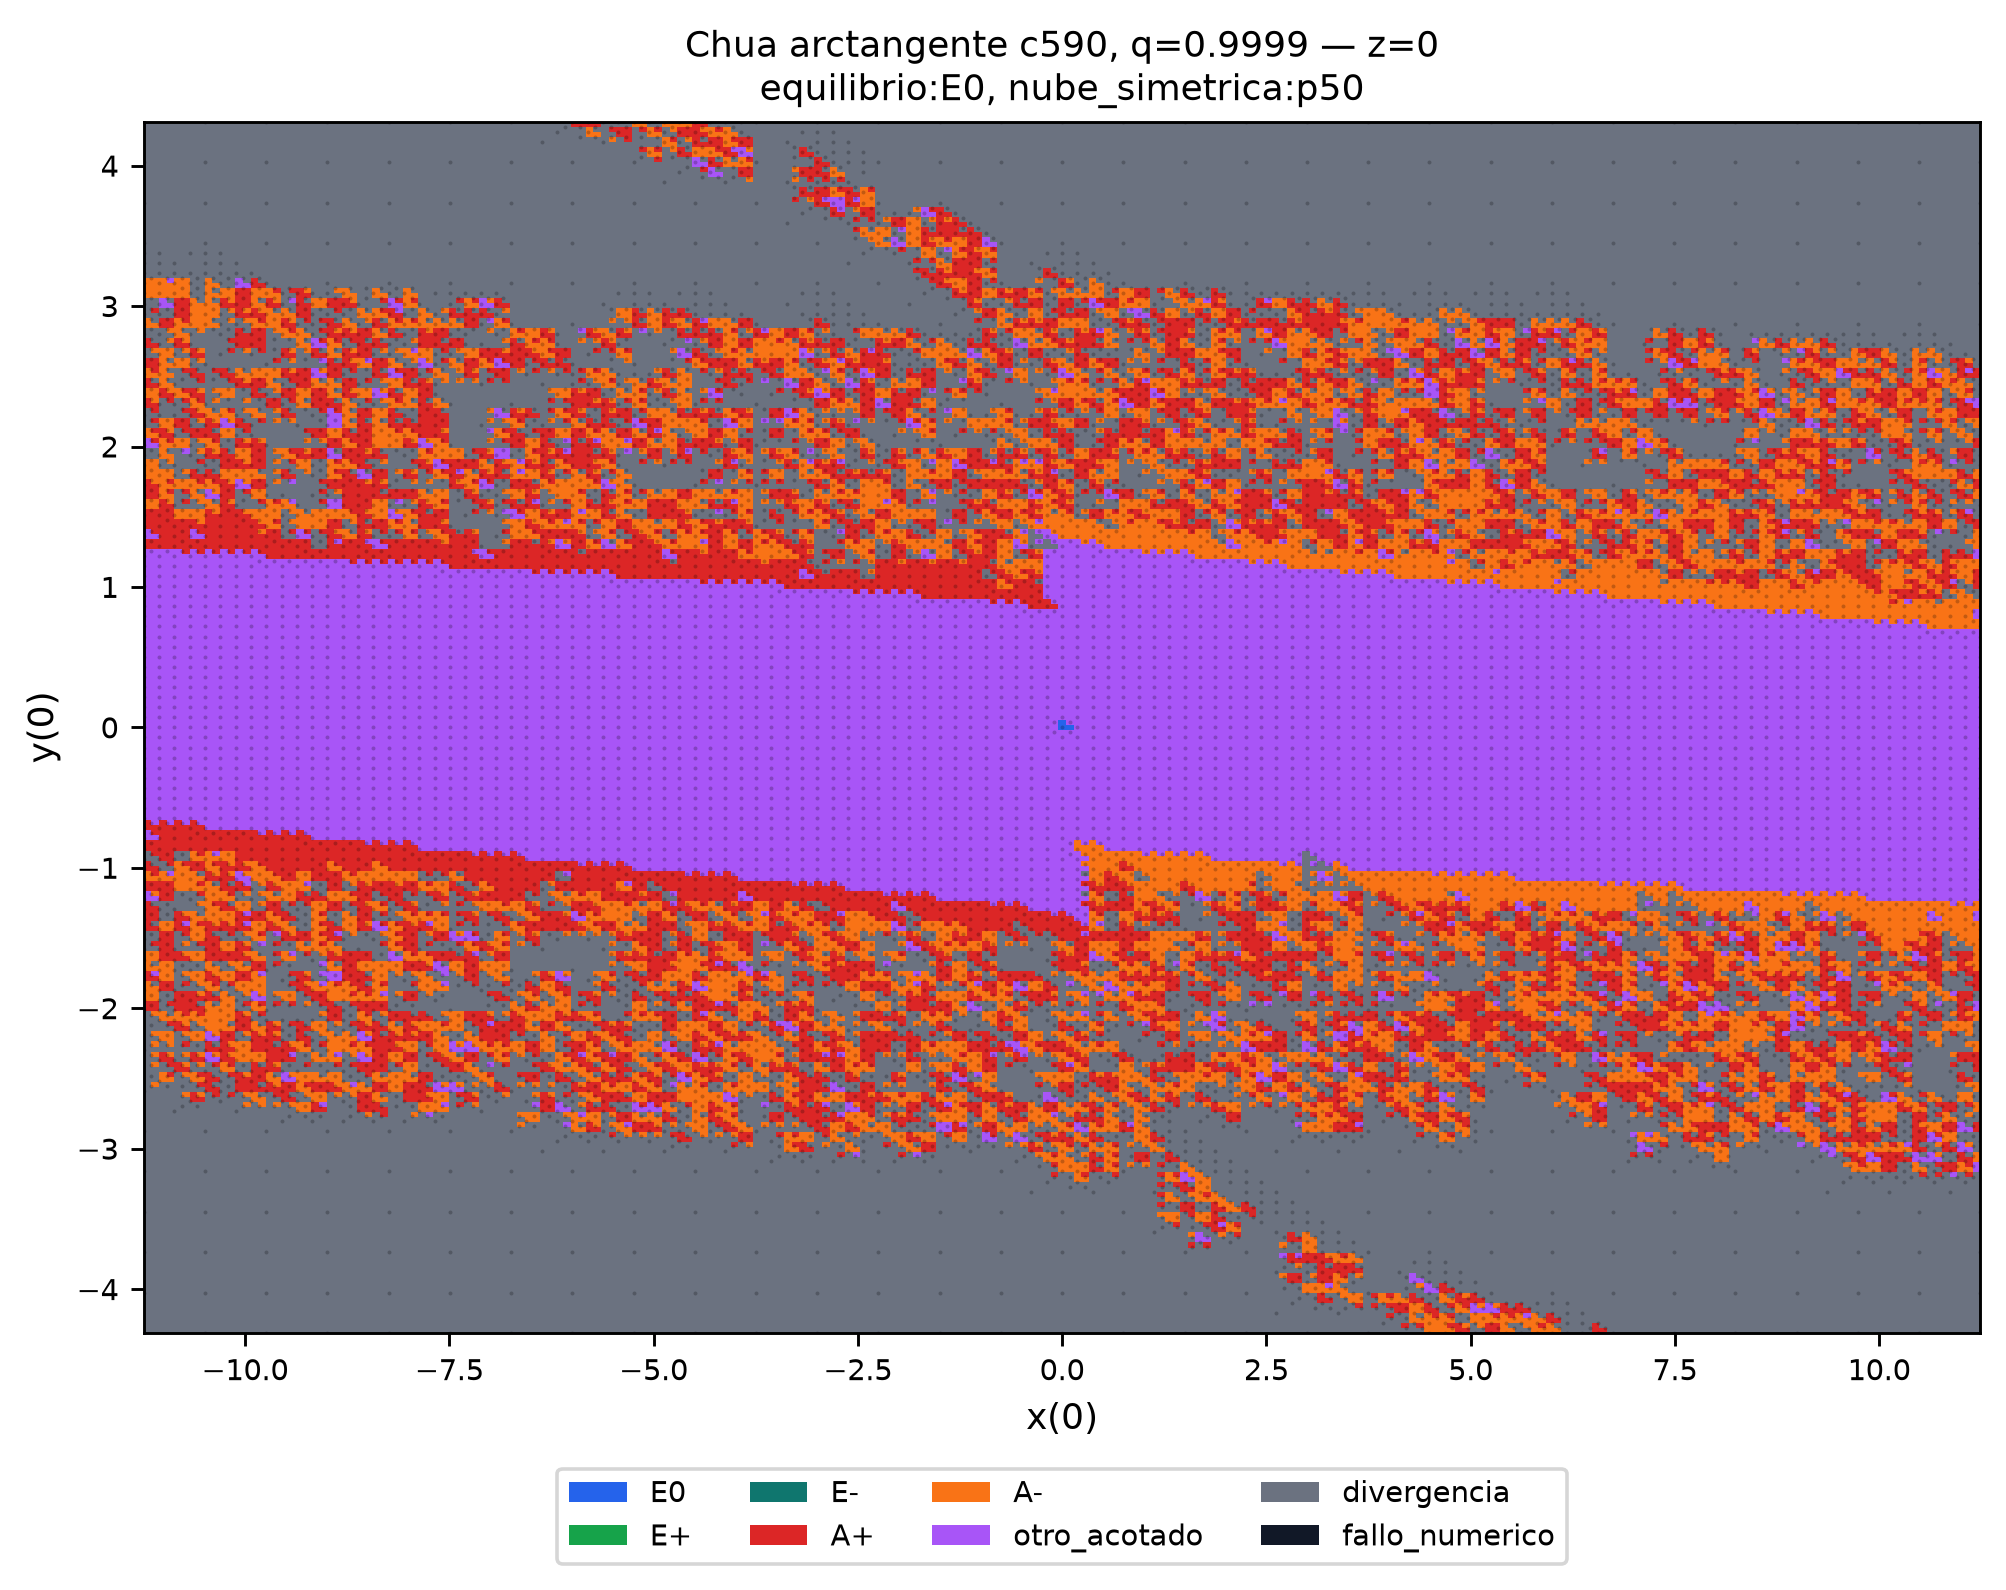
\includegraphics[width=0.94\linewidth,height=0.37\textheight,keepaspectratio]{figures/c590_basin/basin_cut_02.png}\\[-0.25em]
{\footnotesize Corte 3 de las regiones de destino.}
\end{center}
\clearpage
\begin{center}
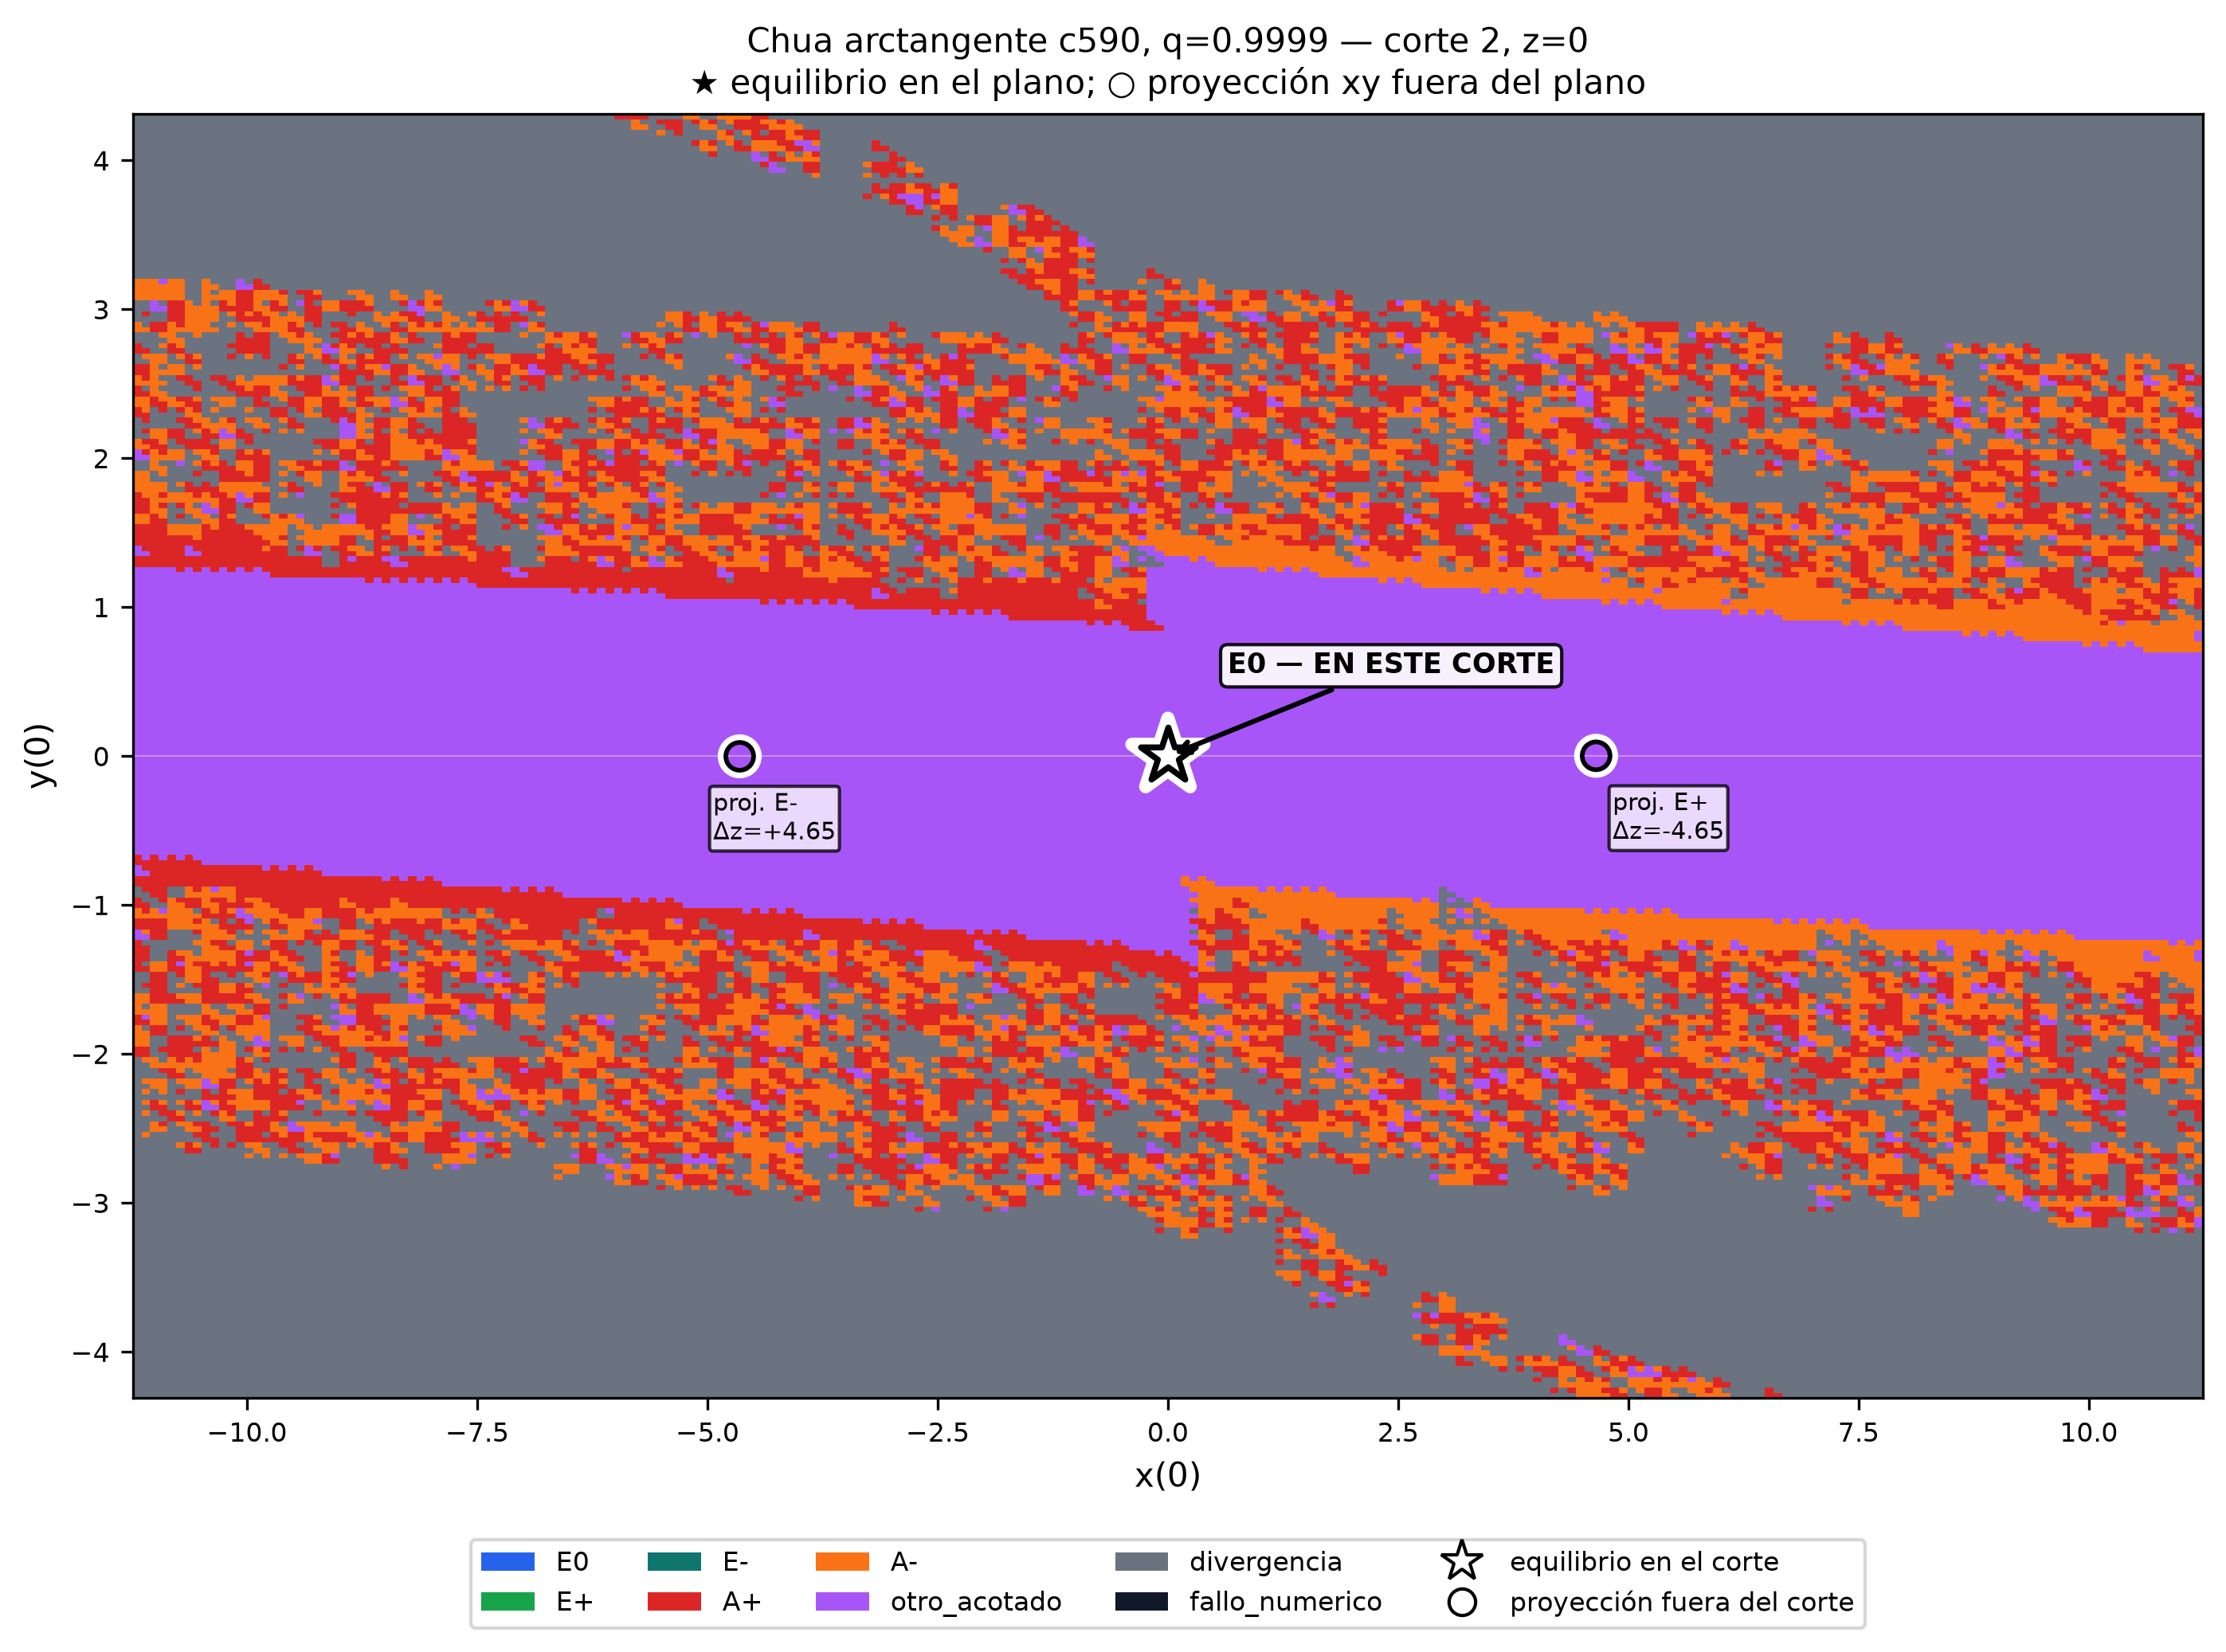
\includegraphics[width=0.94\linewidth,height=0.37\textheight,keepaspectratio]{figures/c590_basin/basin_cut_02_equilibria.png}\\[-0.25em]
{\footnotesize Corte 3 de las regiones de destino y posición de los equilibrios.}
\end{center}
\vfill
\begin{center}
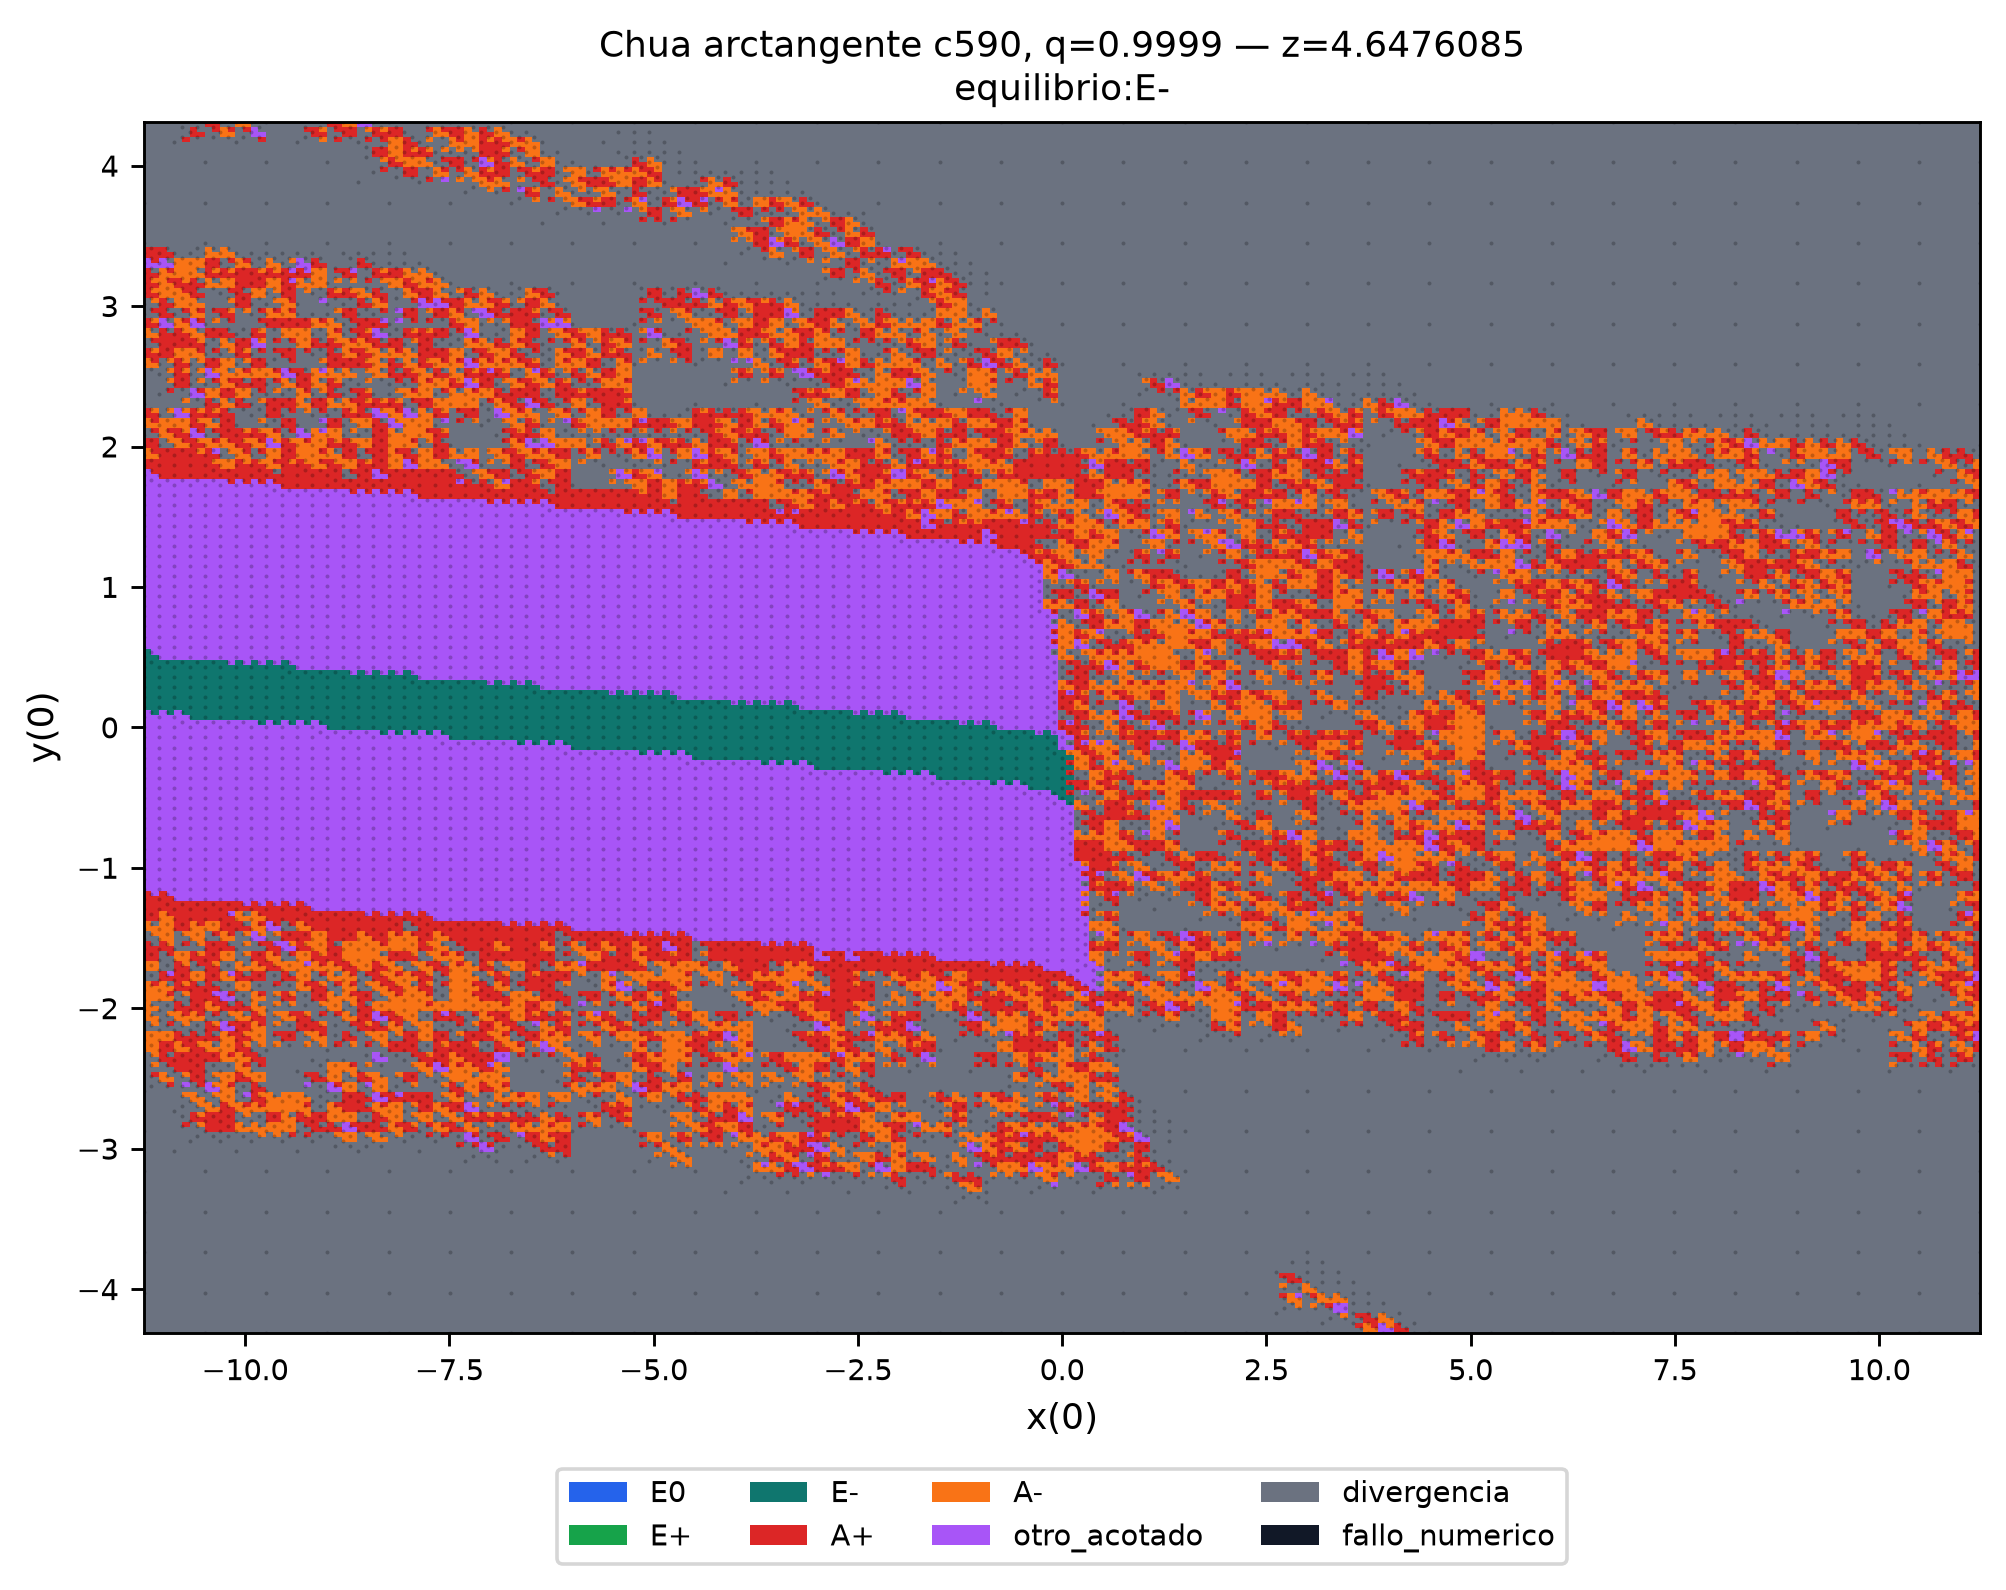
\includegraphics[width=0.94\linewidth,height=0.37\textheight,keepaspectratio]{figures/c590_basin/basin_cut_03.png}\\[-0.25em]
{\footnotesize Corte 4 de las regiones de destino.}
\end{center}
\clearpage
\begin{center}
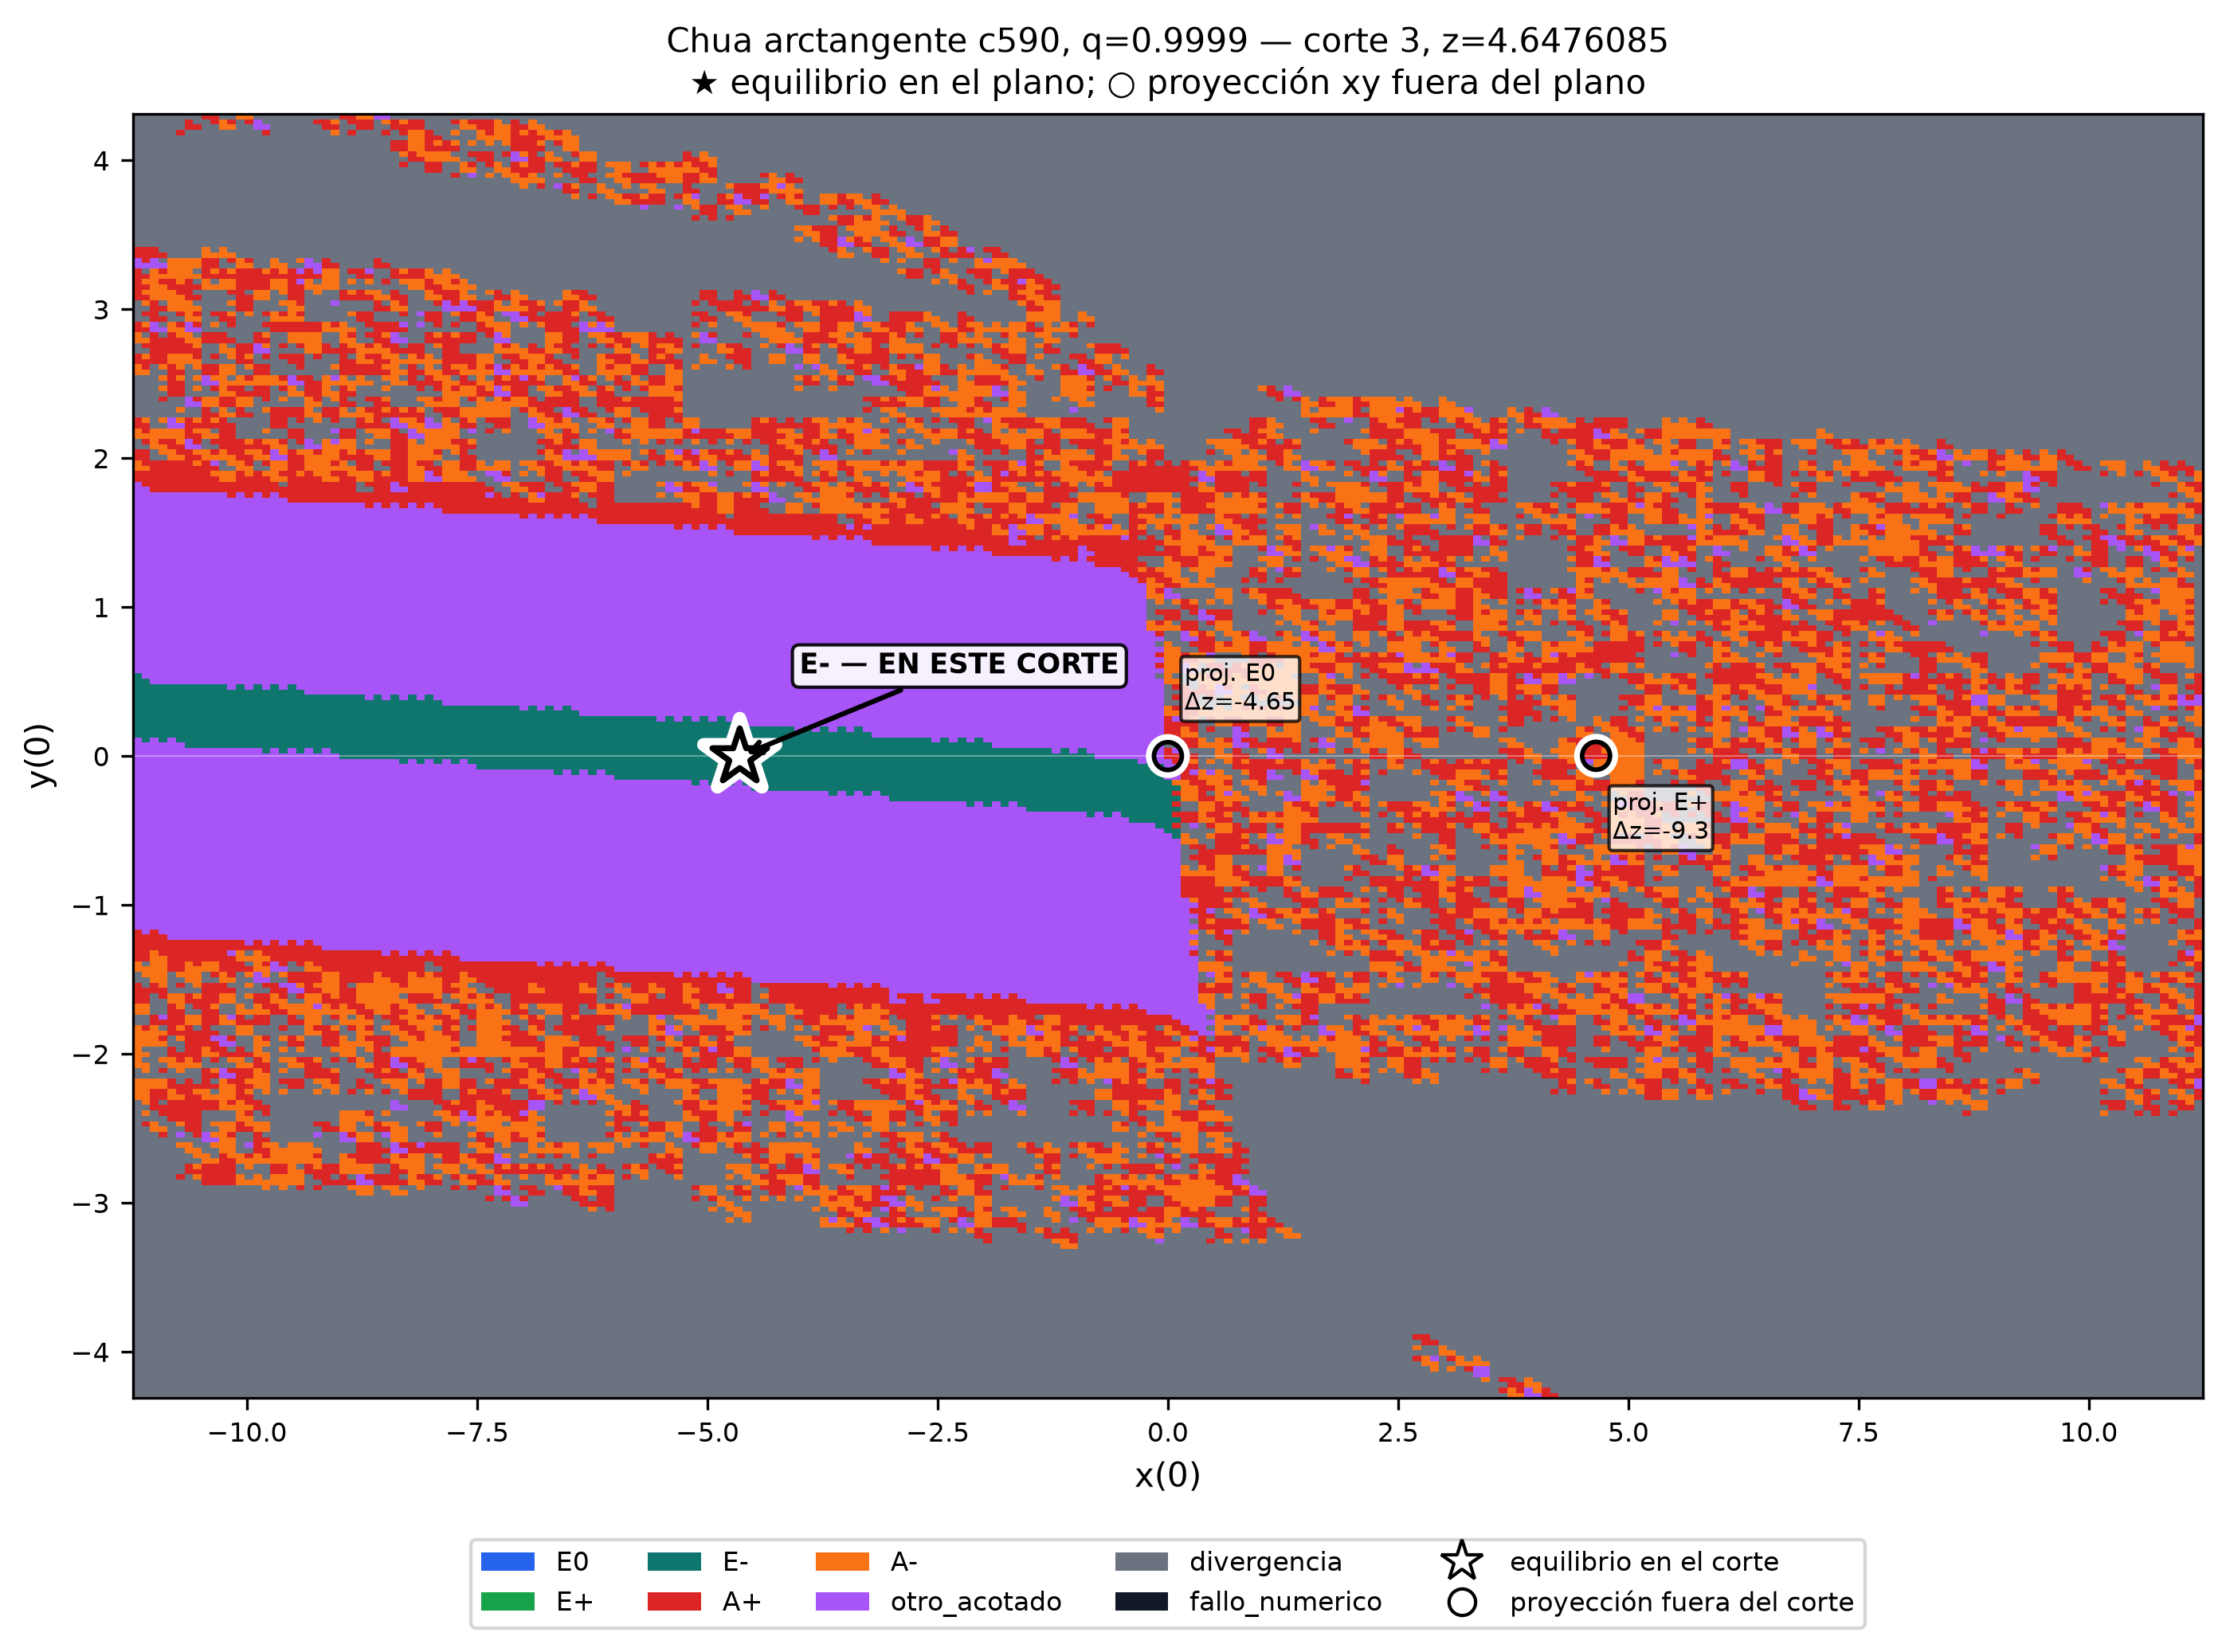
\includegraphics[width=0.94\linewidth,height=0.37\textheight,keepaspectratio]{figures/c590_basin/basin_cut_03_equilibria.png}\\[-0.25em]
{\footnotesize Corte 4 de las regiones de destino y posición de los equilibrios.}
\end{center}
\vfill
\begin{center}
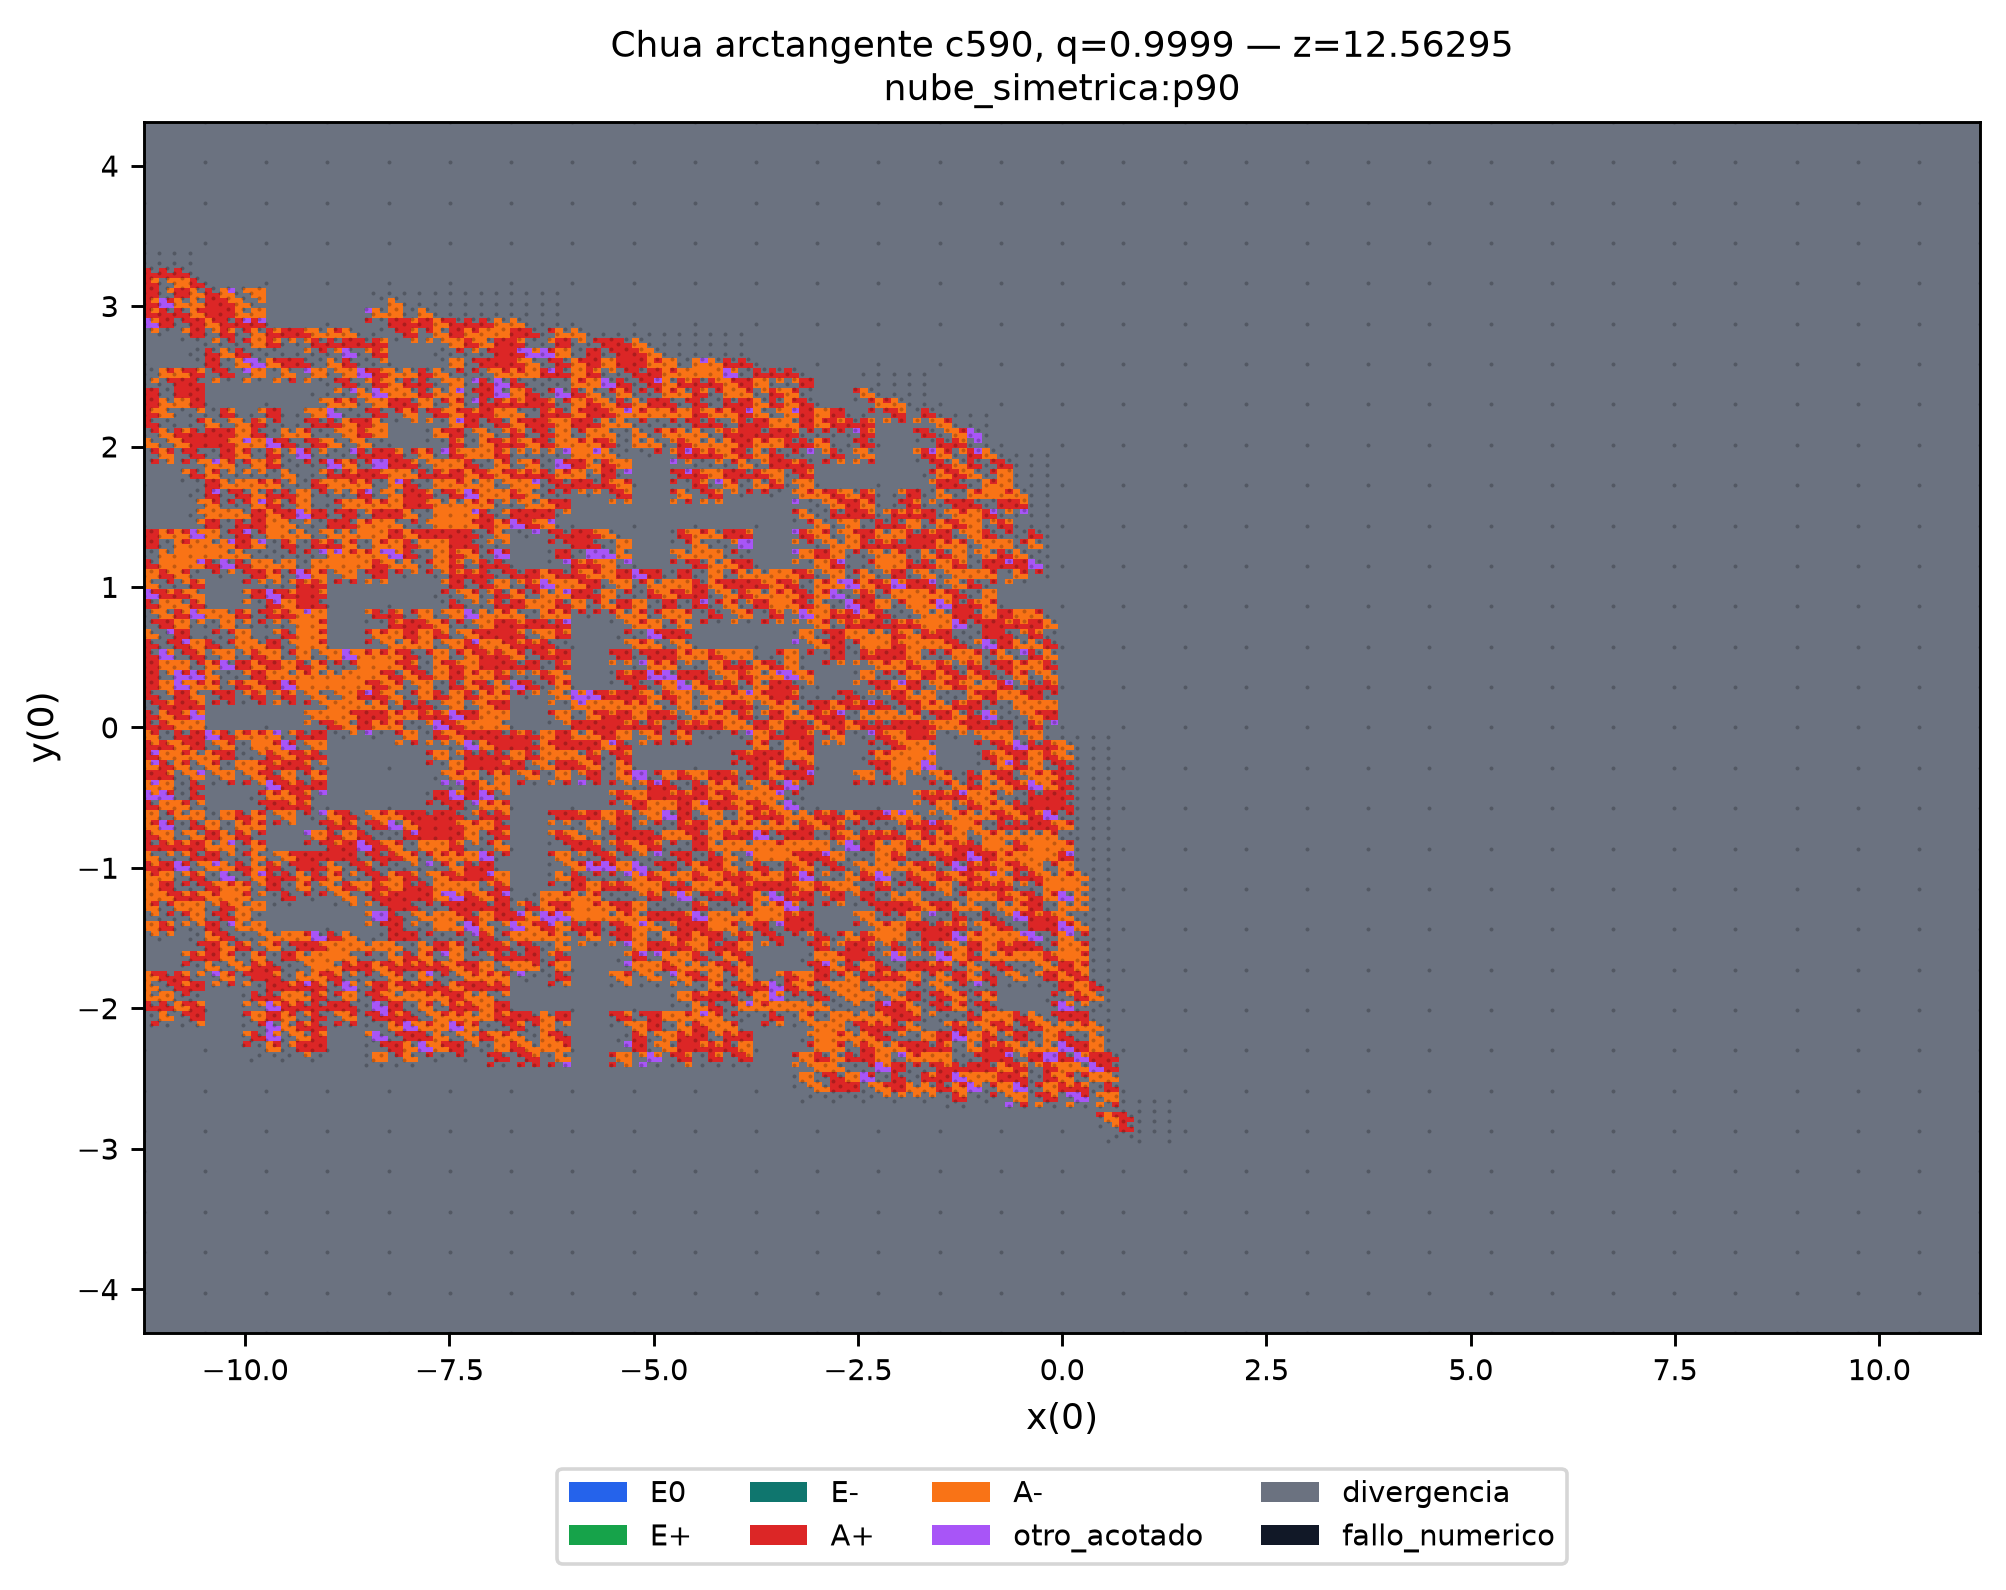
\includegraphics[width=0.94\linewidth,height=0.37\textheight,keepaspectratio]{figures/c590_basin/basin_cut_04.png}\\[-0.25em]
{\footnotesize Corte 5 de las regiones de destino.}
\end{center}
\clearpage
\begin{center}
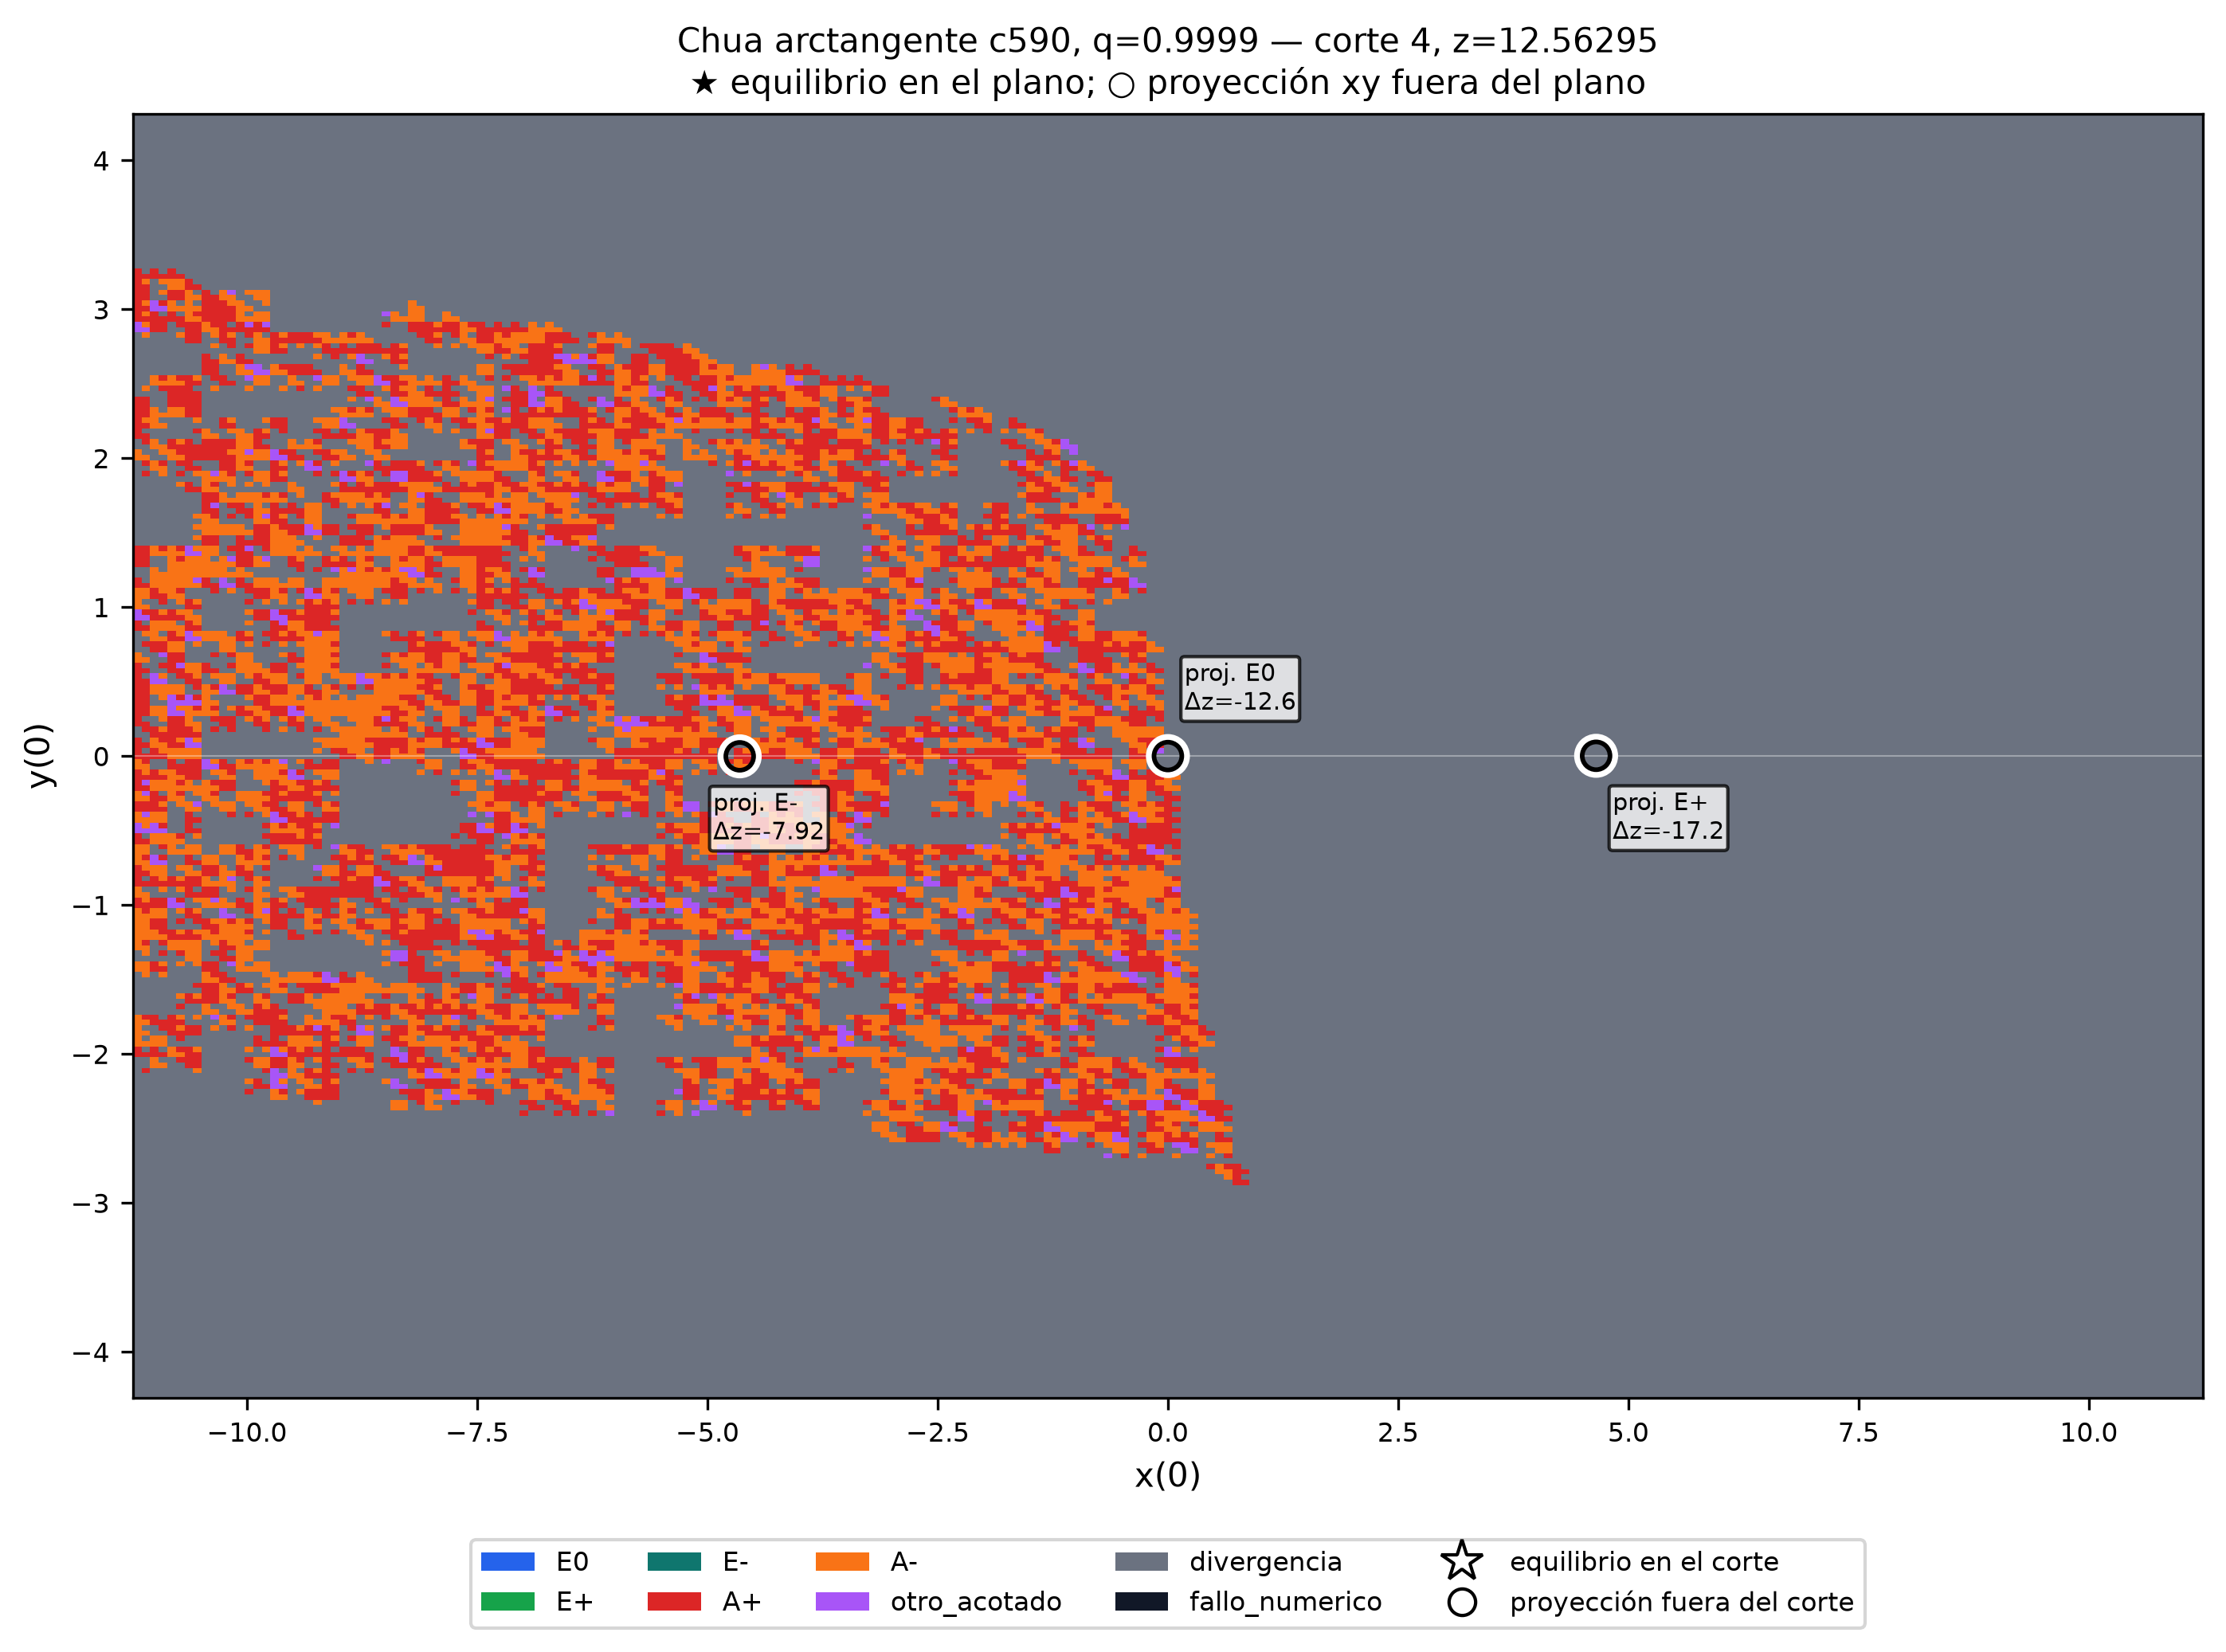
\includegraphics[width=0.94\linewidth,height=0.37\textheight,keepaspectratio]{figures/c590_basin/basin_cut_04_equilibria.png}\\[-0.25em]
{\footnotesize Corte 5 de las regiones de destino y posición de los equilibrios.}
\end{center}
\vfill
\clearpage
\fi
